\documentclass[9pt]{beamer}

% Beamer style
%\usetheme[secheader]{Madrid}
% \usetheme{CambridgeUS}
\useoutertheme{infolines}
\usecolortheme[rgb={0.65,0.15,0.25}]{structure}
% \usefonttheme[onlymath]{serif}
\beamertemplatenavigationsymbolsempty
%\AtBeginSubsection

% Packages
%\usepackage[french]{babel}
\usepackage[latin1]{inputenc}
\usepackage{color}
\usepackage{xspace}
\usepackage{dsfont, stmaryrd}
\usepackage{amsmath, amsfonts, amssymb}
\usepackage{epsfig}
\usepackage{tikz}
\usepackage{url}
\usepackage{/home/robin/LATEX/Biblio/astats}
%\usepackage[all]{xy}
\usepackage{graphicx}

% Maths
% \newtheorem{theorem}{Theorem}
% \newtheorem{definition}{Definition}
\newtheorem{proposition}{Proposition}
% \newtheorem{assumption}{Assumption}
% \newtheorem{algorithm}{Algorithm}
% \newtheorem{lemma}{Lemma}
% \newtheorem{remark}{Remark}
% \newtheorem{exercise}{Exercise}
% \newcommand{\propname}{Prop.}
% \newcommand{\proof}{\noindent{\sl Proof:}\quad}
% \newcommand{\eproof}{$\blacksquare$}

%\renewcommand{\thesection}{\arabic{section}}
%\renewcommand{\thechapter}{\Roman{chapter}}
\setcounter{secnumdepth}{3}
\setcounter{tocdepth}{3}
\newcommand{\pref}[1]{\ref{#1} p.\pageref{#1}}
\newcommand{\qref}[1]{\eqref{#1} p.\pageref{#1}}
\newcommand{\appref}[1]{{\footnotesize{\textcolor{gray}{[\# \ref{#1}]}}}}

% Commands
% \input{TikZcommands.tex}
\definecolor{darkred}{rgb}{0.65,0.15,0.25}
\newcommand{\backupbegin}{
   \newcounter{finalframe}
   \setcounter{finalframe}{\value{framenumber}}
}
\newcommand{\backupend}{
   \setcounter{framenumber}{\value{finalframe}}
}
\newcommand{\emphase}[1]{\textcolor{darkred}{#1}}
% \newcommand{\emphase}[1]{{#1}}
\newcommand{\paragraph}[1]{\textcolor{darkred}{#1}}
\newcommand{\refer}[1]{{\small{\textcolor{blue}{{[\cite{#1}]}}}}}
% \newcommand{\Refer}[1]{{\small{\textcolor{gray}{{[#1]}}}}}
\renewcommand{\newblock}{}

% Symboles
\newcommand{\Beta}{\text{Beta}}
\newcommand{\Bcal}{\mathcal{B}}
\renewcommand{\d}{\;\text{d}}
% \newcommand{\tr}{\text{tr}}
\newcommand{\Cov}{{\mathbb C}\text{ov}}
\newcommand{\Cor}{{\mathbb C}\text{or}}
\newcommand{\cl}{\text{\it c}\ell}
\newcommand{\cst}{\text{cst}}
\newcommand{\Ccal}{\mathcal{C}}
\newcommand{\Dcal}{\mathcal{D}}
\newcommand{\dbf}{{\bf d}}
\newcommand{\Esp}{\xspace\mathbb E}
\newcommand{\Espt}{\widetilde{\Esp}}
\newcommand{\Covt}{\widetilde{\Cov}}
\newcommand{\Ibb}{\mathbb I}
\newcommand{\Ibf}{\mathbf I}
\newcommand{\Hcal}{\mathcal{H}}
\newcommand{\Mt}{\widetilde{M}}
\newcommand{\mt}{\widetilde{m}}
\newcommand{\Mcal}{\mathcal{M}}
\newcommand{\Nbb}{\mathbb{N}}
\newcommand{\Ncal}{\mathcal{N}}
\newcommand{\Obf}{\mathbf 0}
\newcommand{\obs}{\text{obs}}
\newcommand{\pt}{\widetilde{p}}
\newcommand{\Pcal}{\mathcal{P}}
\newcommand{\phibf}{{\boldsymbol{\phi}}}
\newcommand{\Qcal}{\mathcal{Q}}
\newcommand{\Rbb}{\mathbb{R}}
\newcommand{\Sbb}{\mathbb{S}}
\newcommand{\sbf}{\mathbf s}
\newcommand{\st}{\widetilde{s}}
\newcommand{\St}{\widetilde{S}}
\newcommand{\thetabf}{{\boldsymbol{\theta}}}
\newcommand{\Un}{\math{1}}
\newcommand{\Var}{\mathbb V}
\newcommand{\xbf}{\mathbf x}
\newcommand{\Xbf}{\mathbf X}
\newcommand{\Ybf}{\mathbf Y}
\newcommand{\Zbf}{\mathbf Z}

% \newcommand{\diag}{\text{diag}}
\renewcommand{\binom}[2]{{\left(\begin{array}{c}#1 \\ #2 \end{array} \right)}}
\newcommand{\crossprod}[2]{\transpose{#1} \matr{#2}}
\newcommand{\gv}{\, | \,}
\newcommand{\matr}[1]{\boldsymbol{#1}}
\newcommand{\matrbf}[1]{\mathbf{#1}}
\newcommand{\matprod}[2]{\matr{#1} \matr{#2}}
\newcommand{\trace}[1]{\text{tr}\left(#1\right)}
\newcommand{\trans}{\intercal}
\newcommand{\transpose}[1]{\matr{#1}^\trans}
\newcommand{\tcrossprod}[2]{\matr{#1} \transpose{#2}}
\newcommand{\vect}[1]{\matr{#1}} %% un peu inutile
\newcommand{\vectbf}[1]{\matrbf{#1}} %% un peu inutile

\DeclareMathOperator*{\argmin}{arg\,min}
\DeclareMathOperator*{\argmax}{arg\,max}
\DeclareMathOperator{\sign}{sign}
\DeclareMathOperator{\tr}{tr}

\newcommand{\ra}{\emphase{$\rightarrow$} \xspace}

% Hadamard, Kronecker and vec operators
\DeclareMathOperator{\Diag}{Diag} % matrix diagonal
\DeclareMathOperator{\diag}{diag} % vector diagonal
\DeclareMathOperator{\mtov}{vec} % matrix to vector
\newcommand{\kro}{\otimes} % Kronecker product
\newcommand{\had}{\odot}   % Hadamard product

% TikZ
\newcommand{\nodesize}{2em}
\newcommand{\edgeunit}{2.5*\nodesize}
\tikzstyle{hidden}=[draw, circle, fill=gray!50, minimum width=\nodesize, inner sep=0]
\tikzstyle{observed}=[draw, circle, minimum width=\nodesize, inner sep=0]
\tikzstyle{eliminated}=[draw, circle, minimum width=\nodesize, color=gray!50, inner sep=0]
\tikzstyle{empty}=[]
\tikzstyle{arrow}=[->, >=latex, line width=1pt]
\tikzstyle{edge}=[-, line width=1pt]
\tikzstyle{dashedarrow}=[->, >=latex, dashed, line width=1pt]
\tikzstyle{lightarrow}=[->, >=latex, line width=1pt, fill=gray!50, color=gray!50]


% Directory
\newcommand{\fignet}{/home/robin/Bureau/RECHERCHE/RESEAUX/EXPOSES/FIGURES}
\newcommand{\figchp}{/home/robin/Bureau/RECHERCHE/RUPTURES/EXPOSES/FIGURES}
\newcommand{\figfig}{../figs}


%====================================================================
%====================================================================

%====================================================================
%====================================================================
\begin{document}
%====================================================================
%====================================================================

%====================================================================
\title{An introduction to Bayesian statistical inference}

\author{S. Robin}

\institute[INRA / AgroParisTech / Paris-Saclay]{
  INRA / AgroParisTech /univ. Paris-Saclay 
  }

\date[JC(2)BIM]{JC(2)BIM, June 2018, Fr�jus}

%====================================================================
%====================================================================
\maketitle
%====================================================================

\frame{\frametitle{Outline} \tableofcontents}

%====================================================================
%====================================================================
\frame{ \frametitle{Reminder: Joint, marginal, conditional (1/2)} \label{app:JointMargCond}

  \paragraph{Reminder:} 2 loci with 2 alleles each: $(A, a)$, $(B, b)$
  \begin{itemize}
   \item Joint distribution: 
   $$
   \begin{array}{c|cc|c}
   & B & b & \text{marginal} \\
   \hline
   A & f_{AB} & f_{Ab} & p_A = f_{AB} + f_{Ab} \\
   a & f_{aB} & f_{ab} & p_a = f_{aB} + f_{ab} \\
   \hline
   \text{marginal} & q_B = f_{AB} + f_{aB} & q_b = f_{Ab} + f_{ab} & 
    f_{AB} + f_{Ab} + f_{aB} + f_{ab} = 1 
  \end{array}
  $$ \\ ~
  \item Marginal distribution: 'integrate out' the allele of the other locus
  $$
  \Pr\{B\} = q_B = f_{AB} + f_{aB}
  $$ \\ ~
  \item Conditional distribution: fix the allele of the other locus
  $$
  \Pr\{A \gv b\} = \frac{\Pr\{A, b\}}{\Pr\{b\}} = \frac{f_{Ab}}{q_b} = \frac{f_{Ab}}{f_{Ab} + f_{ab}}
  $$
  ('Bayes formula')
  \end{itemize}
}

%====================================================================
\frame{ \frametitle{Reminder: Joint, marginal, conditional  (2/2)} \label{app:JointMargCond}

  \paragraph{Continuous case:} 2 continuous random variables $U$ and $V$
  \begin{itemize}
   \item Joint distribution: 
   $$
   \begin{array}{c|c|c}
   & v  & \text{marginal} \\
   \hline & & \\
   u & p_{UV}(u, v) & p_U(u) = \int p_{UV}(u, v) \d v \\ & & \\
   \hline & & \\
   \text{marginal} & p_V(v) = \int p_{UV}(u, v) \d u & \int p_{UV}(u, v) \d u \d v = 1 
   \end{array}
  $$ \\ ~
  \item Marginal distribution: 'integrate out' the other variable
  $$
  p_U(u) = \int p_{UV}(u, v) \d v
  $$ \\ ~
  \item Conditional distribution: fix the value of the other variable
  $$
  p_{V|U=u}(v) = \frac{p_{UV}(u, v)}{p_U(u)} = \frac{p_{UV}(u, v)}{\int p_{UV}(u, v) \d v}
  $$
  \end{itemize}

}


%====================================================================
\section{Statistical inference: Bayesian point-of-view} \label{sec:Intro}
\frame{\frametitle{Outline} \tableofcontents[currentsection]}
%====================================================================
\subsection{Statistical inference: frequentist / Bayesian}
\frame{\frametitle{Outline} \tableofcontents[currentsubsection]}
%====================================================================
\frame{ \frametitle{An example}

  \paragraph{Example:} 
  \begin{itemize}
   \item $n$ patients: $i = 1 \dots n$
   \item $Y_i =$ status (0 = healthy, 1 = sick) of patient $i$ 
   \item $\xbf_i = (x_{i1}, \dots x_{ip}) =$ vector of gene expression for patient $i$ (gene $j = 1 \dots p$)
  \end{itemize}
  
  \bigskip \bigskip 
  \paragraph{Dataset:} $n = 78$, $p=15$
  \begin{center} {\tt \begin{tabular}{lrrrcr}
  & AB033066  & NM003056  & NM000903  & \dots & Status \\ 
  \hline 
  1  & 0.178  & 0.116  & 0.22  & & 0 \\ 
  2  & 0.065  & -0.073  & -0.014  & & 0 \\ 
  3  & -0.077  & 0.03  & 0.043  & & 0 \\ 
  4  & 0.176  & -0.041  & 0.362  & & 0 \\ 
  5  & -0.089  & -0.164  & -0.266  & & 0 
  \end{tabular} } \end{center}
  
  \pause \bigskip \bigskip 
  Similar question for genotyping data.
  }
  
%====================================================================
\frame{ \frametitle{A statistical model}

  \paragraph{Logistic regression} Logistic regression
  \begin{itemize}
   \item The patients are independent.
   \item The probability for patient $i$ to be sick depends on $\xbf_i$:
   $$
   \Pr\{Y_i = 1\} = \frac{e^{\xbf_i^\intercal \thetabf}}{1 + e^{\xbf_i^\intercal \thetabf}}, 
   \qquad \qquad
   \xbf_i^\intercal \thetabf = \sum_{j=1}^p x_{ij} \theta_j
   $$
   \item $\thetabf = (\theta_1, \dots \theta_p):$ unknown parameter (regression coefficients, incl. intercept)
  \end{itemize}
  
  $$
  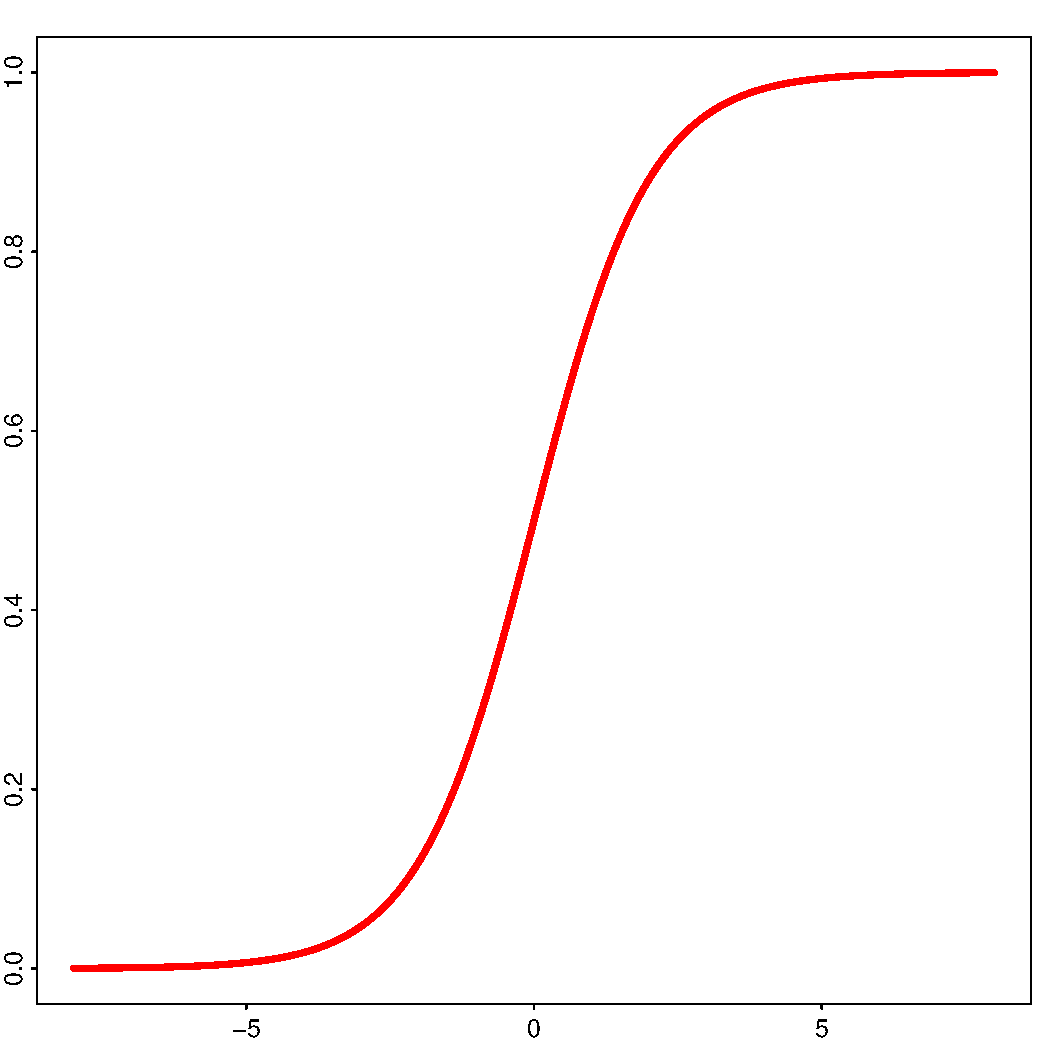
\includegraphics[width=.6\textwidth, height=.4\textheight]{\figfig/logistic-curve}
  $$
}  

%====================================================================
\frame{ \frametitle{Frequentist inference}

  \paragraph{$\thetabf =$ fixed parameter:}
  \begin{itemize}
   \item Statistical model:
   $$
   \Ybf \sim p_\thetabf
   $$
   \item Inference: get a (point) estimate $\widehat{\thetabf}$ e.g.
   $$
   \widehat{\thetabf}: \qquad \log p_{\widehat{\thetabf}}(\Ybf) = \max_\thetabf \log p_{\thetabf}(\Ybf)
   $$
   \item The estimate $\widehat{\thetabf}$ itself is random (depends on the data) \ra confidence interval, tests, ...
  \end{itemize}
  
  \bigskip \bigskip \pause
  \paragraph{Output:} {\tt GLM = glm(Y $\sim$ X, family=binomial)}
  \begin{center} {\tt \begin{tabular}{lrrrr}
    & Estimate  & Std. Error  & z value  & Pr($>|$z$|$) \\ 
    \hline 
    (Intercept)  & -0.7212697  & 0.6512707  & -1.107481  & 0.2680861 \\ 
    XAB033066  & 7.23375  & 2.505118  & 2.887589  & 0.003882068 \\ 
    XNM003056  & -0.6116423  & 1.854695  & -0.3297806  & 0.7415658 \\ 
    XNM000903  & 1.732625  & 1.199888  & 1.443988  & 0.1487423 \\
    \dots
    \end{tabular} } \end{center}
}

%====================================================================
\frame{ \frametitle{Bayesian inference}

  \paragraph{$\thetabf =$ random parameter:}
  \begin{itemize}
   \item Statistical model:
   $$
   \emphase{\ell(\Ybf \gv \thetabf)} := p(\Ybf \gv \thetabf) \qquad \text{($=$ {\sl likelihood})}
   $$
   \item Inference: provide the conditional distribution of $\thetabf$ given the observed data $\Ybf$:
   $$
   p(\thetabf \gv \Ybf) \qquad \text{($=$ {\sl posterior} distribution)}
   $$
   \ra credibility intervals
   \item Requires to define a marginal distribution: 
   $$
   \emphase{\pi(\thetabf)} := p(\thetabf) \qquad \text{($=$ {\sl prior} distribution)}
   $$  
  \end{itemize}
}

%====================================================================
\subsection{Basics of Bayes inference}
\frame{\frametitle{Outline} \tableofcontents[currentsubsection]}
%====================================================================
\frame{ \frametitle{Why 'Bayes'}

  \paragraph{Bayes formula:}
  $$
  P(A \gv B) = \frac{P(A, B)}{P(B)} = \frac{P(A)}{P(B)} P(B \gv A)
  $$
  \begin{itemize}
   \item $P(B) =$ marginal probability of $B$
   \item $P(A, B) =$ joint probability of $A$ and $B$
   \item $P(A \gv B) =$ conditional probability of $A$ given $B$ \appref{app:JointMargCond}
  \end{itemize}

  \bigskip \bigskip \pause
  \paragraph{Be careful.} Many methods, e.g.
  $$
  \text{Bayesian network, Naive Bayes, ...}
  $$
  \begin{itemize}
  \item use conditional probabilities
  \item but have nothing to do with Bayesian inference (in the statistical sense)
  \end{itemize}
}

%====================================================================
\frame{ \frametitle{Bayes formula for Bayesian inference (1/2)}

  \paragraph{Posterior distribution.}
  $$
  p(\thetabf \gv \Ybf) = \frac{p(\Ybf, \thetabf)}{p(\Ybf)} = \frac{\overset{prior}{\overbrace{\pi(\thetabf)}} \; \overset{likelihood}{\overbrace{\ell(\Ybf \gv \thetabf)}}}{\emphase{p(\Ybf)}}
  $$
  \ra Requires to evaluate the {\sl integrated likelihood} (i.e. marginal)
  $$
  p(\Ybf) = \int \pi(\thetabf) \ell(\Ybf \gv \thetabf) \d \thetabf,
  $$
  which act as the normalizing constant of the posterior $p(\thetabf \gv \Ybf)$.
}

%====================================================================
\frame{ \frametitle{Bayes formula for Bayesian inference (2/2)}

  \paragraph{Some remarks.}
  \begin{enumerate}
   \item \pause $p(\cdot)$ is sometimes denoted $[\cdot]$:
   $$
   p(\thetabf \gv \Ybf) = \frac{\pi(\thetabf) \; \ell(\Ybf \gv \thetabf)}{p(\Ybf)}
   \qquad \Leftrightarrow \qquad
   [\thetabf \gv \Ybf] = \frac{[\thetabf] \; [\Ybf \gv \thetabf]}{[\Ybf]}
   $$ \\ ~
   \item \pause Computing $p(\Ybf)$ is generally (very) difficult: see Section \ref{sec:MCMC} \\~
   \item \pause Obviously
   $$
   p(\thetabf \gv \Ybf) \propto \pi(\thetabf) \; \ell(\Ybf \gv \thetabf),
   $$
   \ra $p(\thetabf \gv \Ybf)$ and $p(\thetabf' \gv \Ybf)$ can be compared, \emphase{without computing $p(\Ybf)$} \\~
   \item \pause Obviously, the posterior $p(\thetabf \gv \Ybf)$ depends on the prior $\pi(\thetabf)$ (see next slides).
  \end{enumerate}

}
%====================================================================
\frame{ \frametitle{The posterior depends on the prior} \label{slide:prior}

  \begin{tabular}{cc}
    \begin{tabular}{p{.5\textwidth}}
    \paragraph{Data \& Model:}
    \begin{itemize}
     \item $Y_i =1$ if sick, $0$ otherwise
     \item $n = 10$ patients
     \item $\vdots:$ number sicks $/ n$
    \end{itemize}

    \bigskip \pause
    \paragraph{Param:}
    \begin{itemize}
     \item $\theta =$ proba. sick
     \item $\textcolor{blue}{\boldsymbol{-}}:$ prior $\pi(\theta)$
    \end{itemize}

    \bigskip \pause
    \paragraph{Output:}
    \begin{itemize}
     \item $\boldsymbol{-}:$  posterior $p(\theta \gv \Ybf)$
    \end{itemize}

    \end{tabular}
    & 
    \hspace{-.02\textwidth}
    \begin{tabular}{p{.5\textwidth}}
	 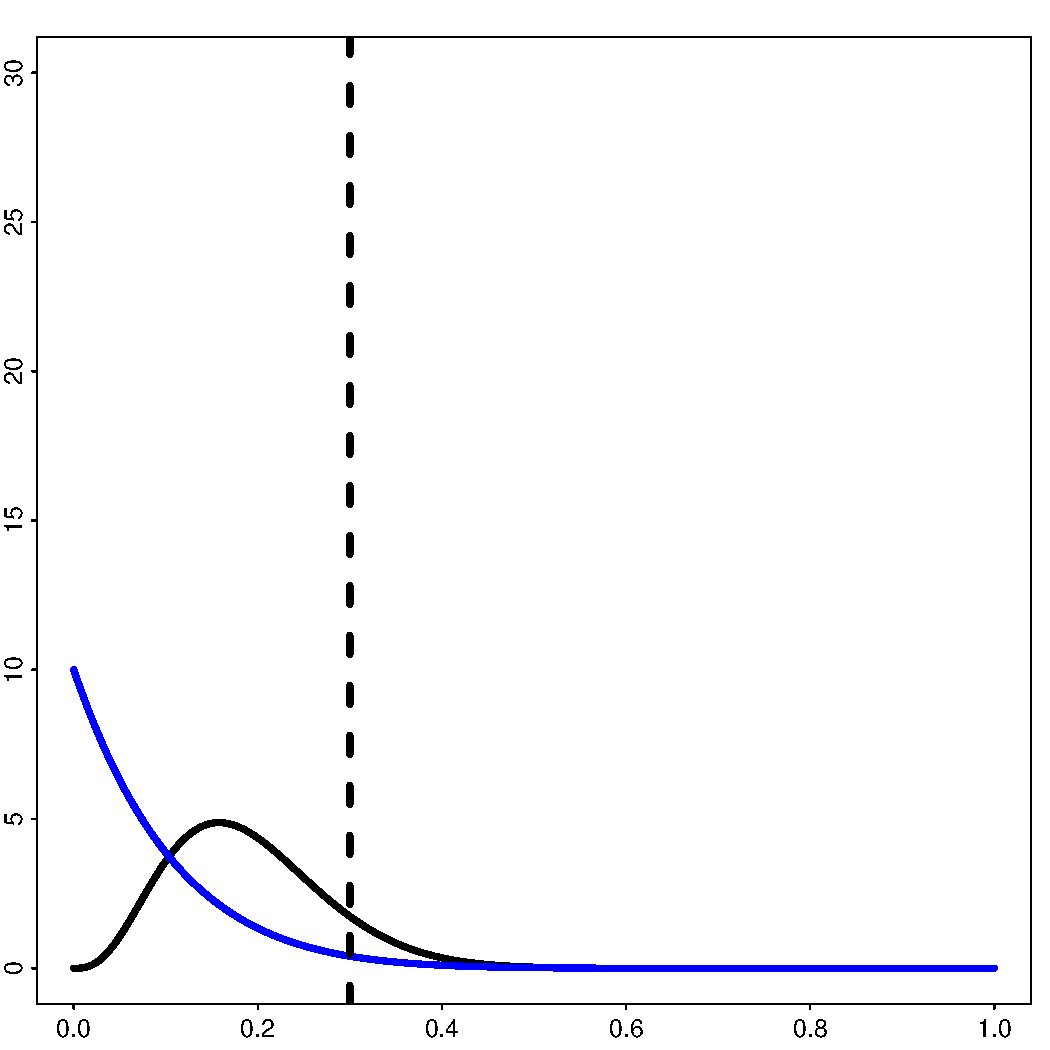
\includegraphics[width=.3\textwidth, height=.3\textheight]{../figs/beta-binomial-a1-b10-n10-p33} \\
	 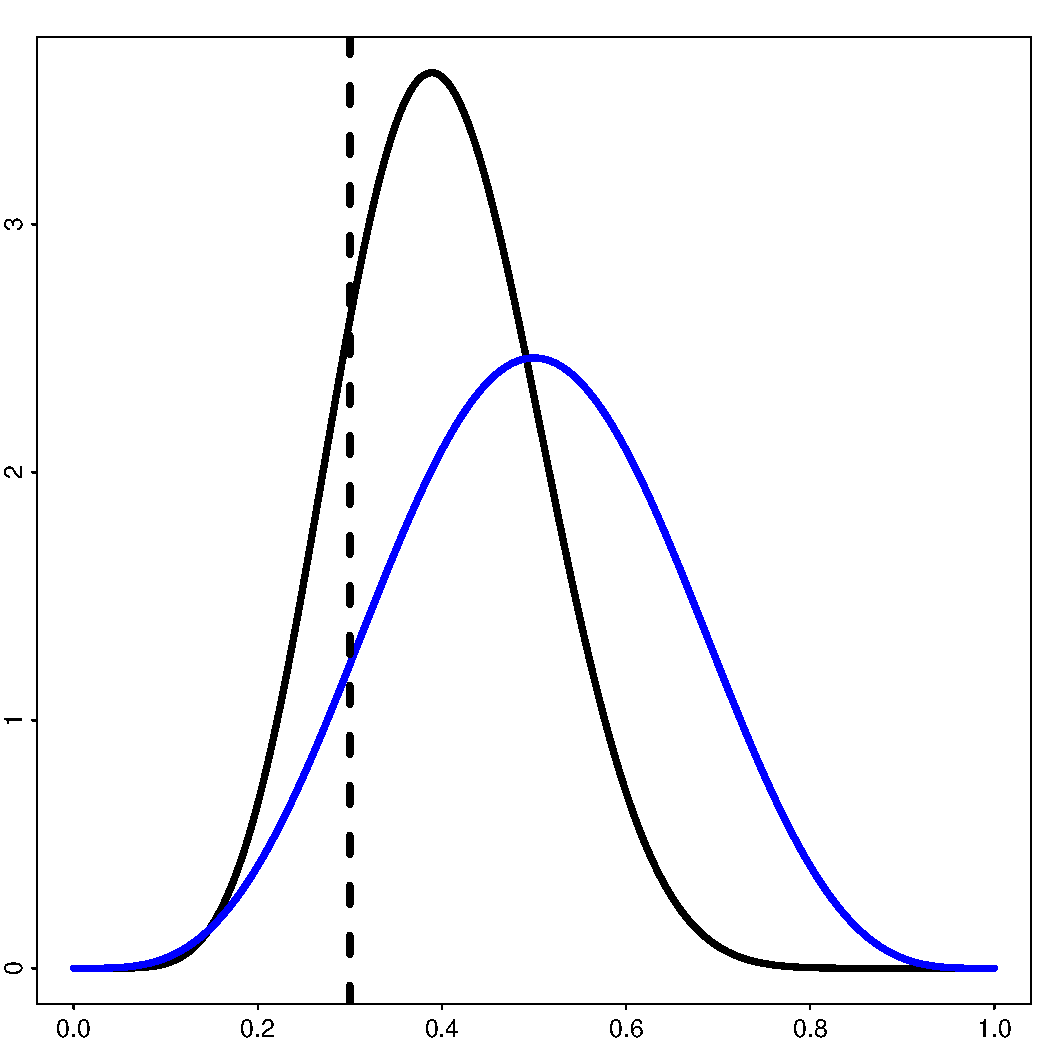
\includegraphics[width=.3\textwidth, height=.3\textheight]{../figs/beta-binomial-a5-b5-n10-p33} \\
	 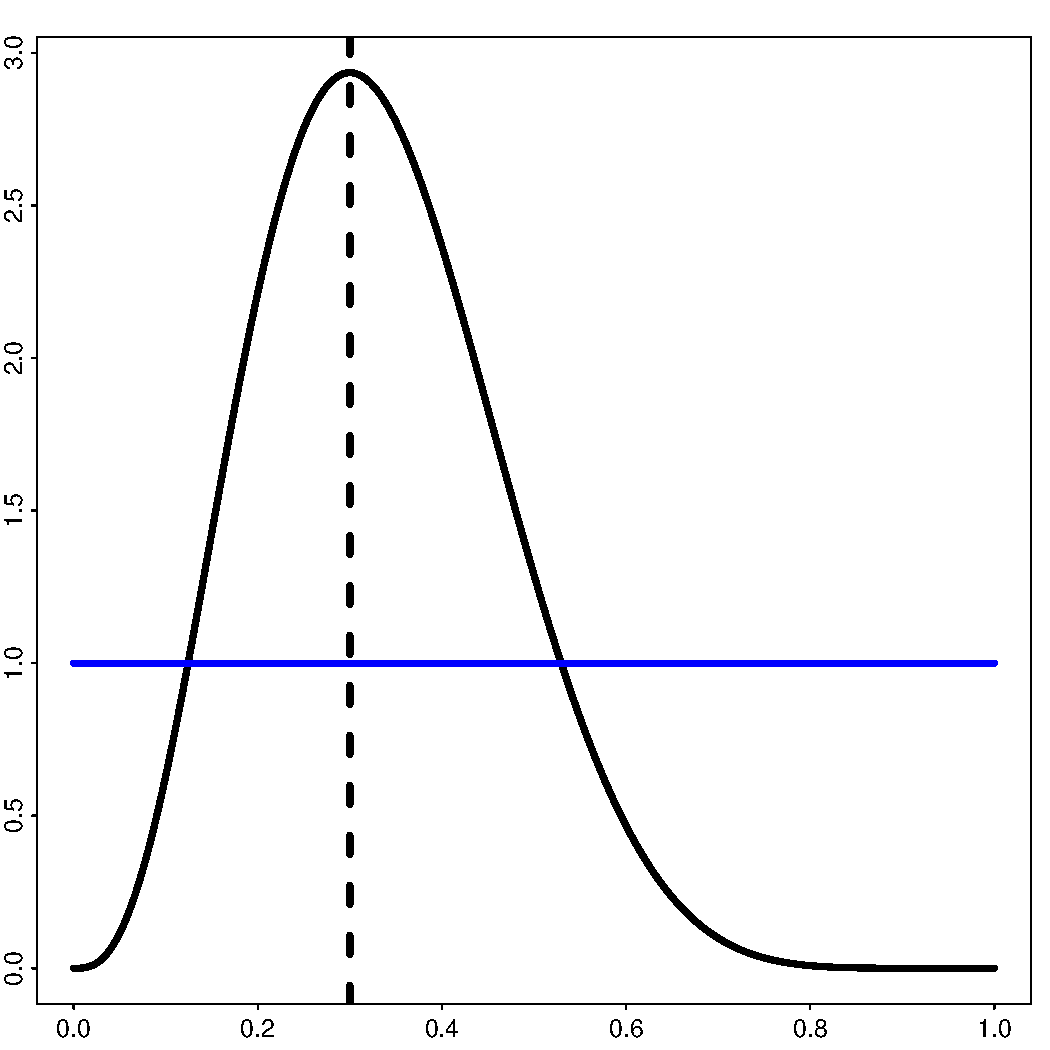
\includegraphics[width=.3\textwidth, height=.3\textheight]{../figs/beta-binomial-a1-b1-n10-p33} 
    \end{tabular}
  \end{tabular}
}

%====================================================================
\frame{ \frametitle{Dependency vanishes when $n$ increases}

  \begin{tabular}{ccc}
    $n = 10$ & $n = 100$ & $n = 1000$ \\
	 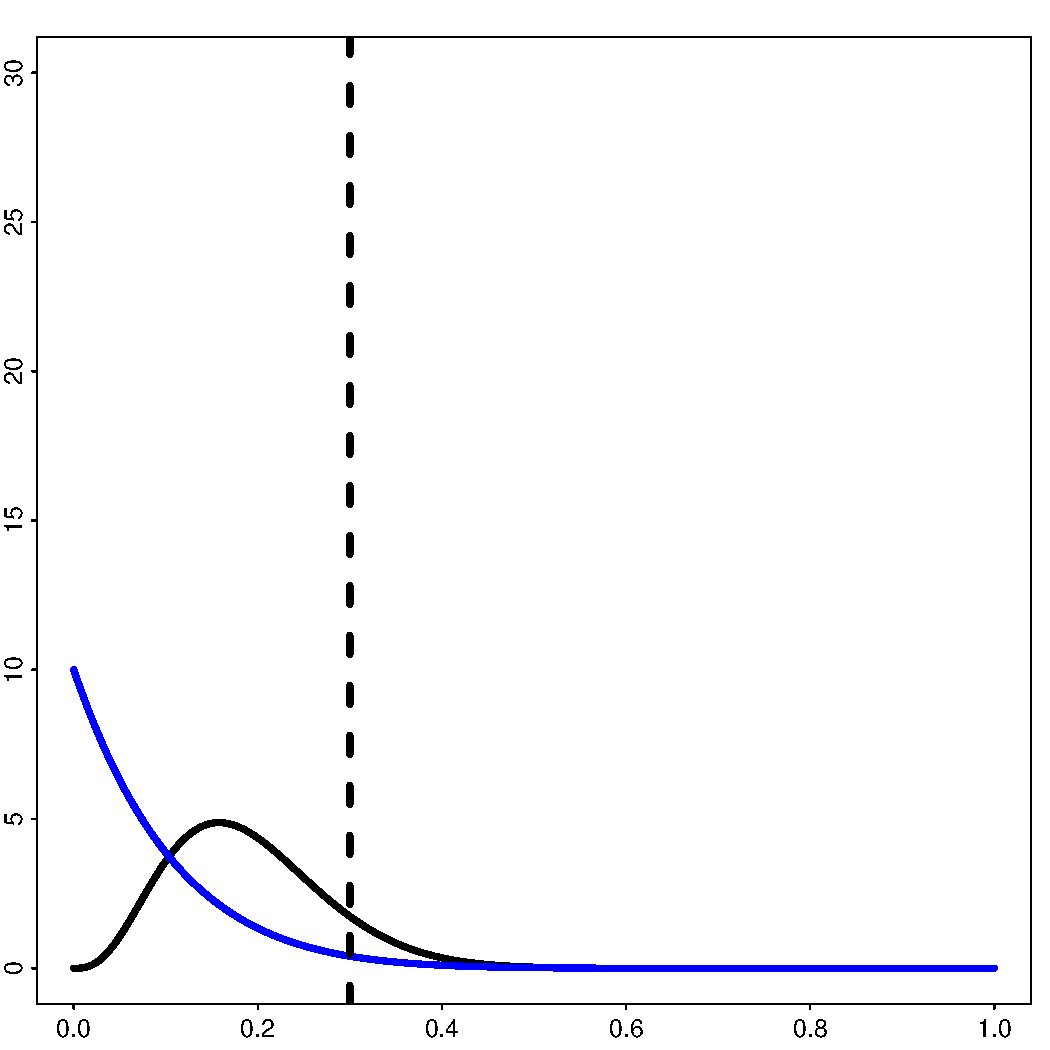
\includegraphics[width=.3\textwidth, height=.25\textheight]{../figs/beta-binomial-a1-b10-n10-p33} & 
	 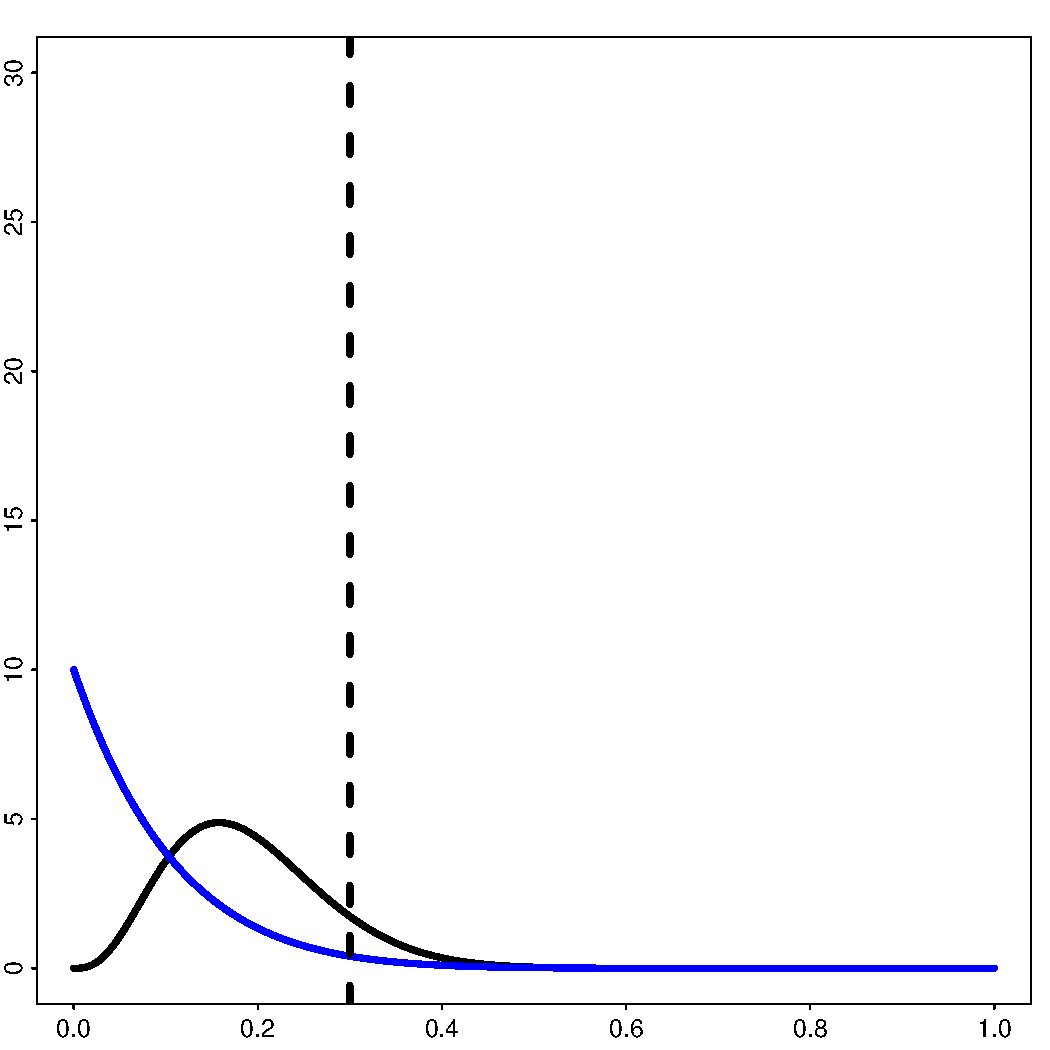
\includegraphics[width=.3\textwidth, height=.25\textheight]{../figs/beta-binomial-a1-b10-n10-p33} 
	 & 
	 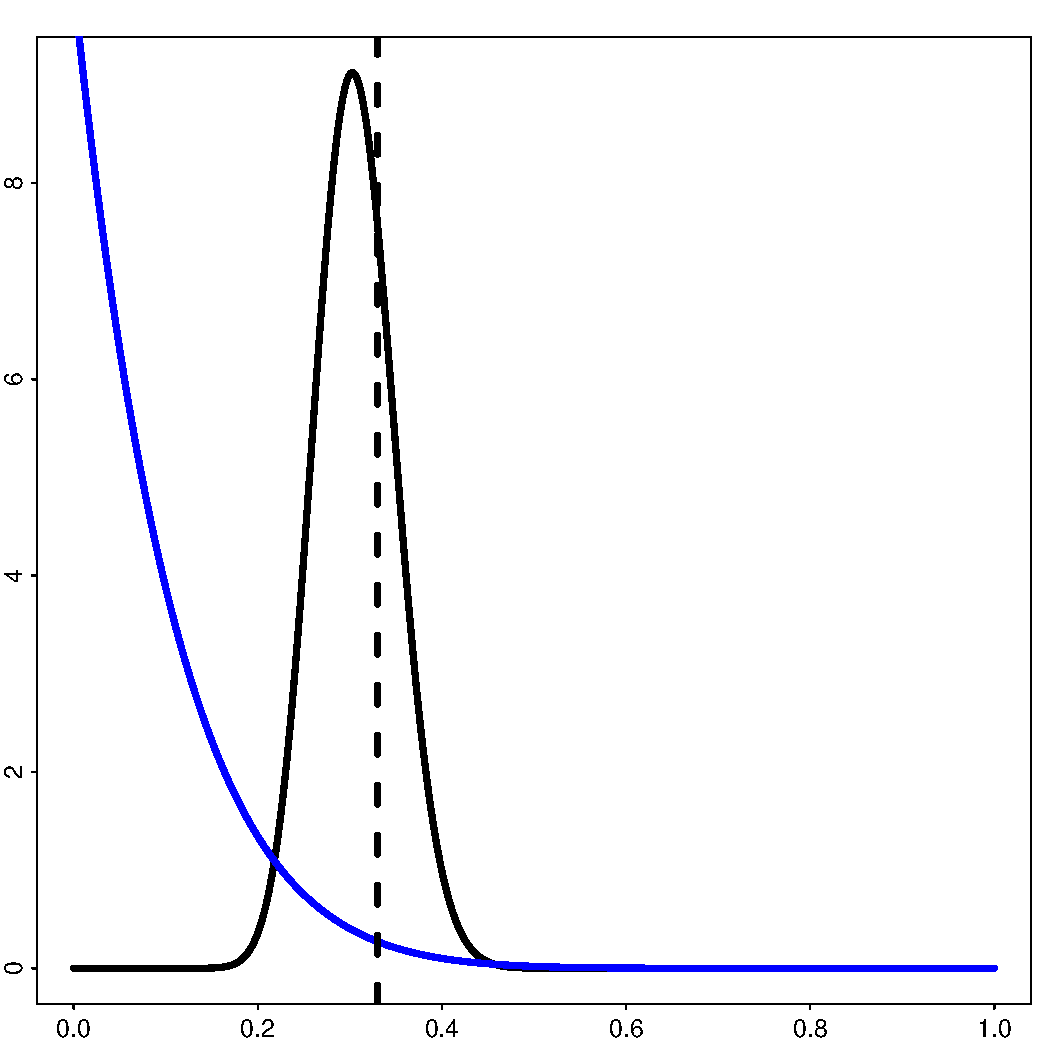
\includegraphics[width=.3\textwidth, height=.25\textheight]{../figs/beta-binomial-a1-b10-n100-p33} 
	 \\
	 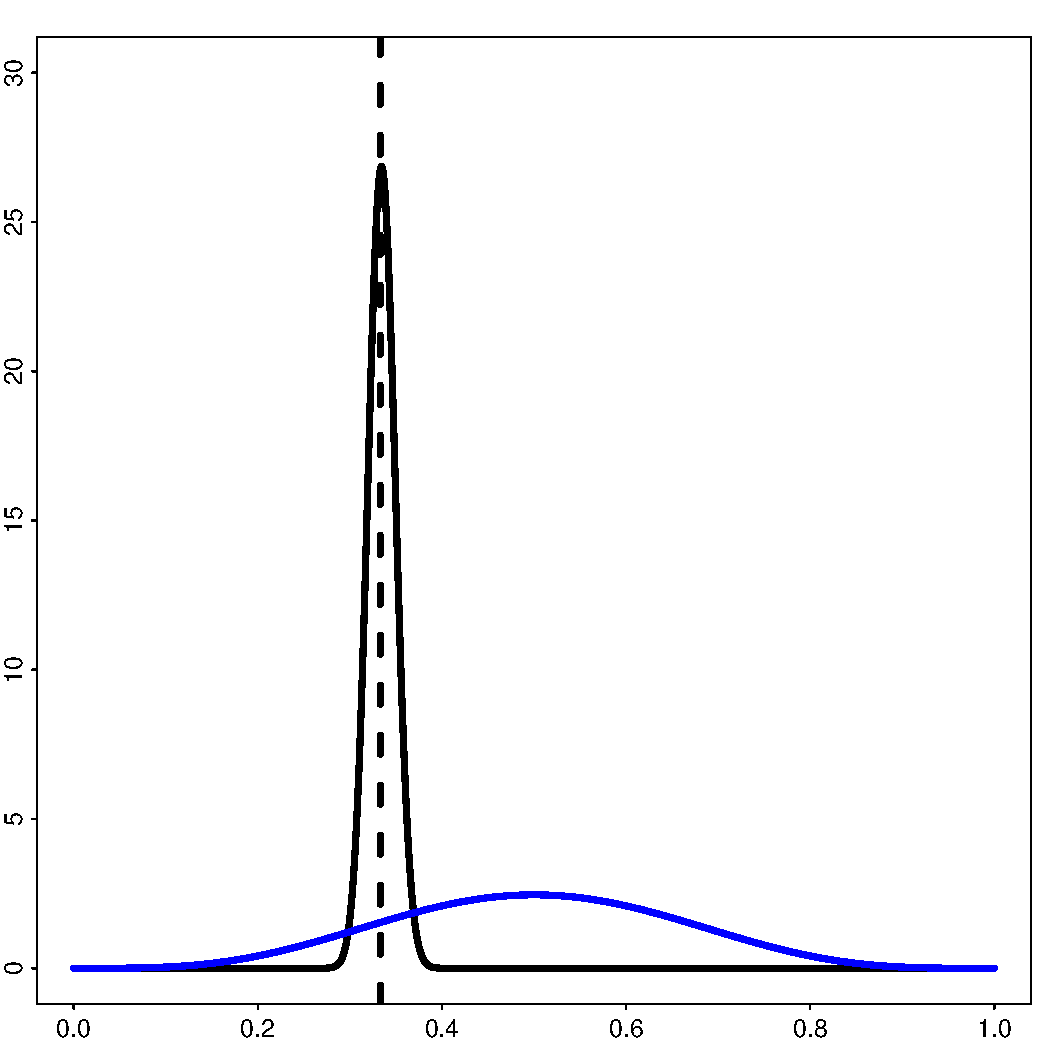
\includegraphics[width=.3\textwidth, height=.25\textheight]{../figs/beta-binomial-a5-b5-n1000-p33} & 
	 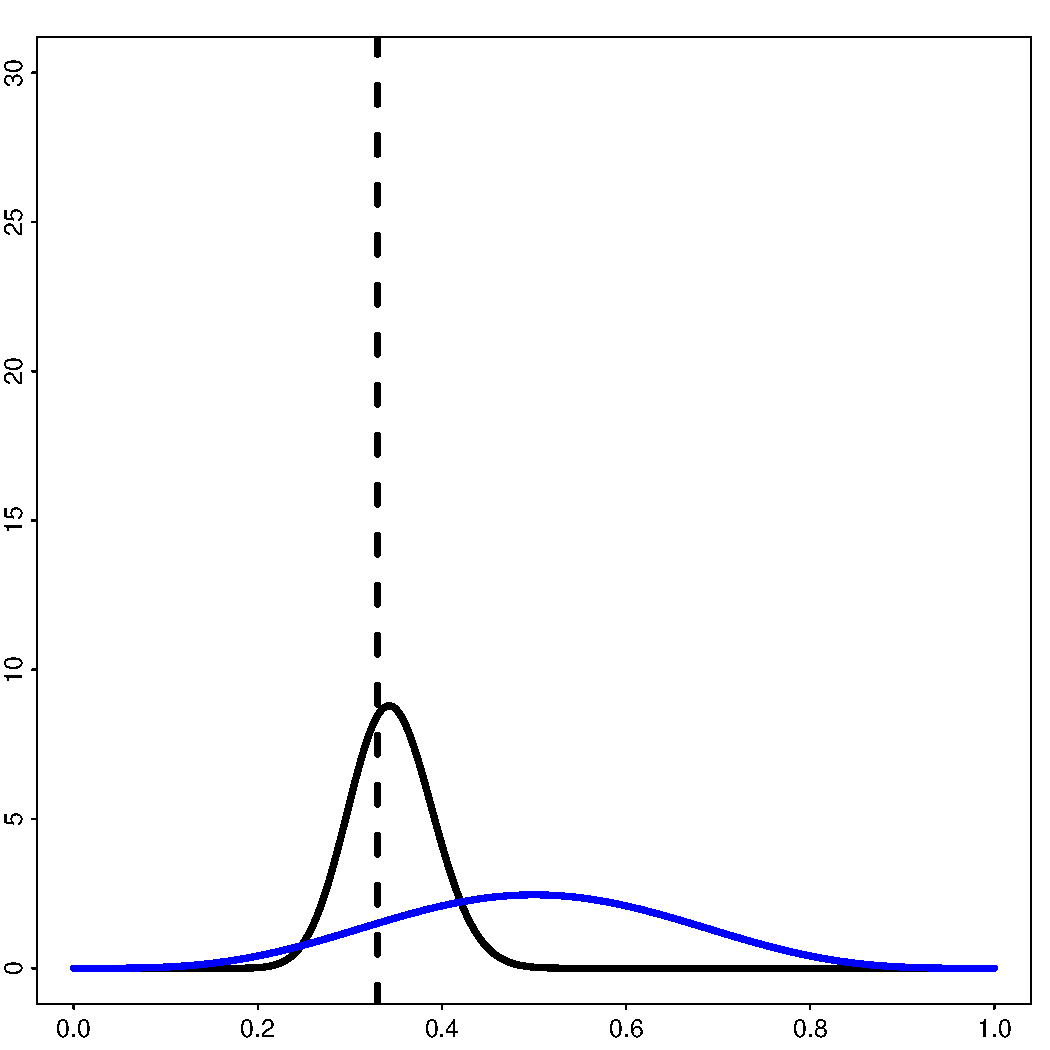
\includegraphics[width=.3\textwidth, height=.25\textheight]{../figs/beta-binomial-a5-b5-n100-p33} 
	 & 
	 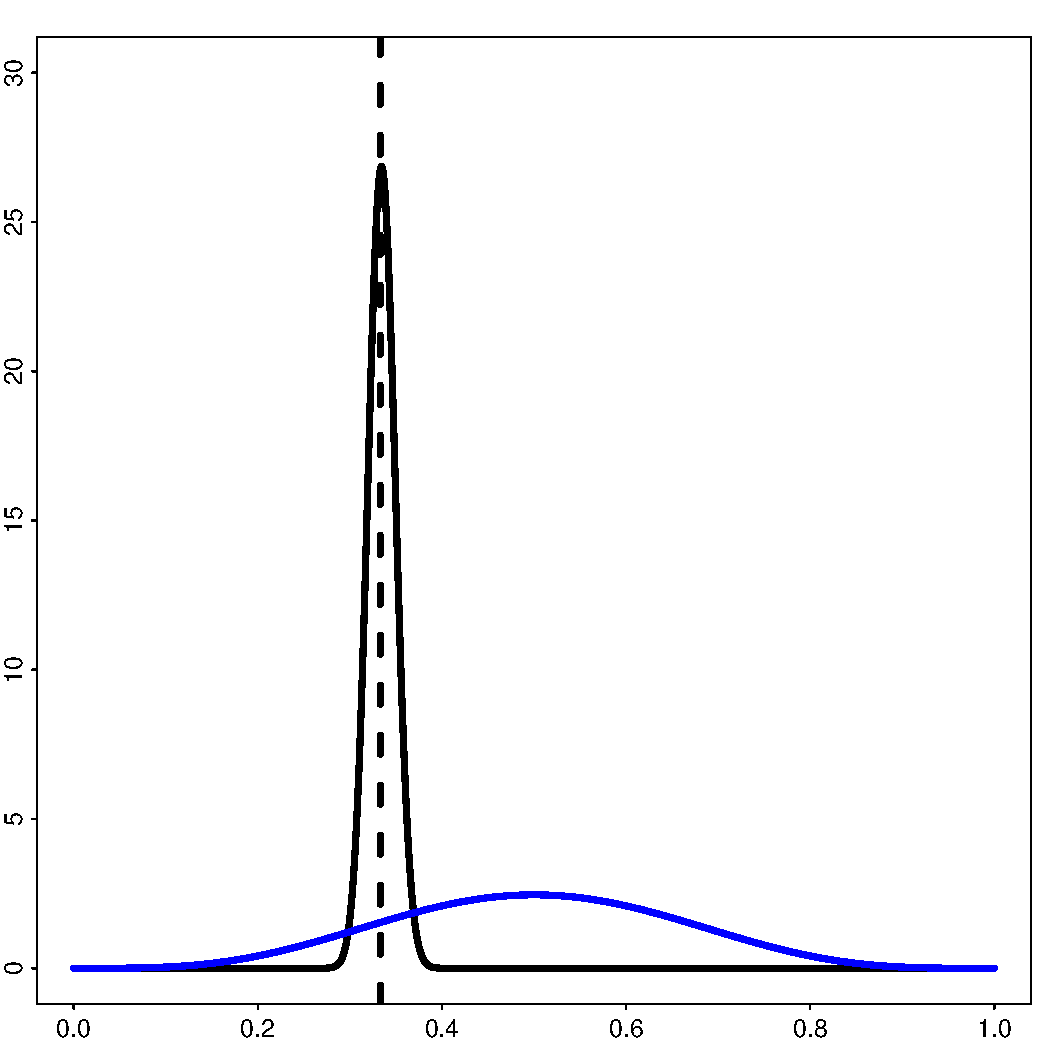
\includegraphics[width=.3\textwidth, height=.25\textheight]{../figs/beta-binomial-a5-b5-n1000-p33} 
	 \\
	 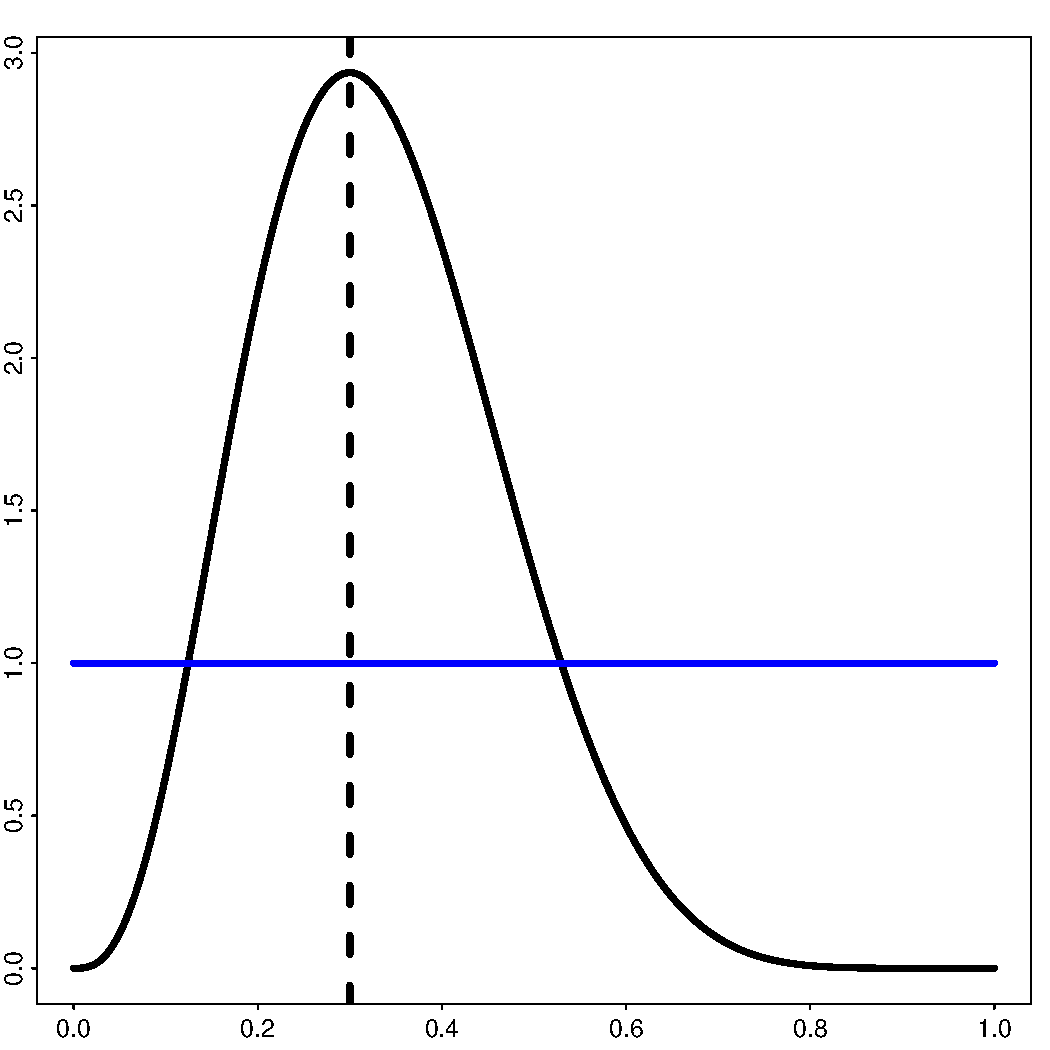
\includegraphics[width=.3\textwidth, height=.25\textheight]{../figs/beta-binomial-a1-b1-n10-p33} & 
	 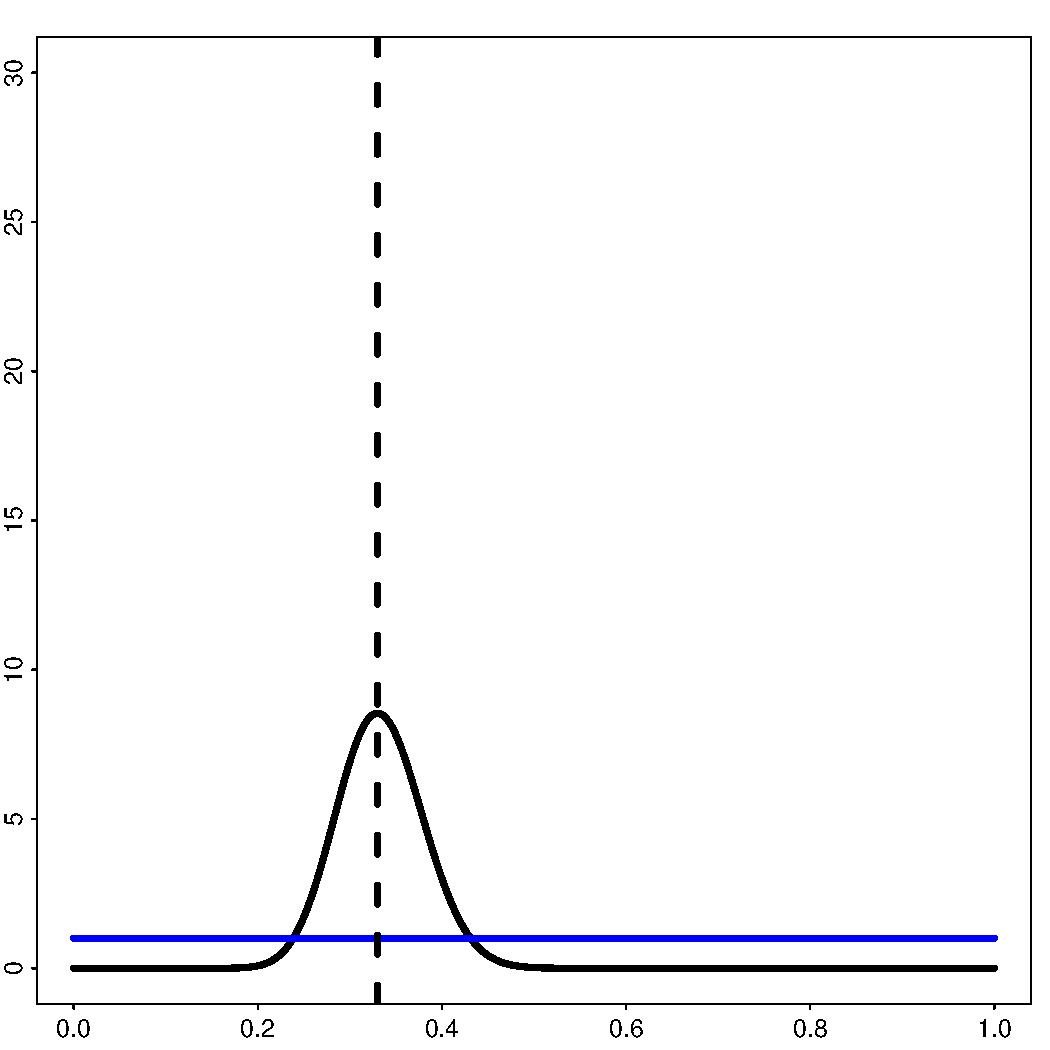
\includegraphics[width=.3\textwidth, height=.25\textheight]{../figs/beta-binomial-a1-b1-n100-p33} 
	 & 
	 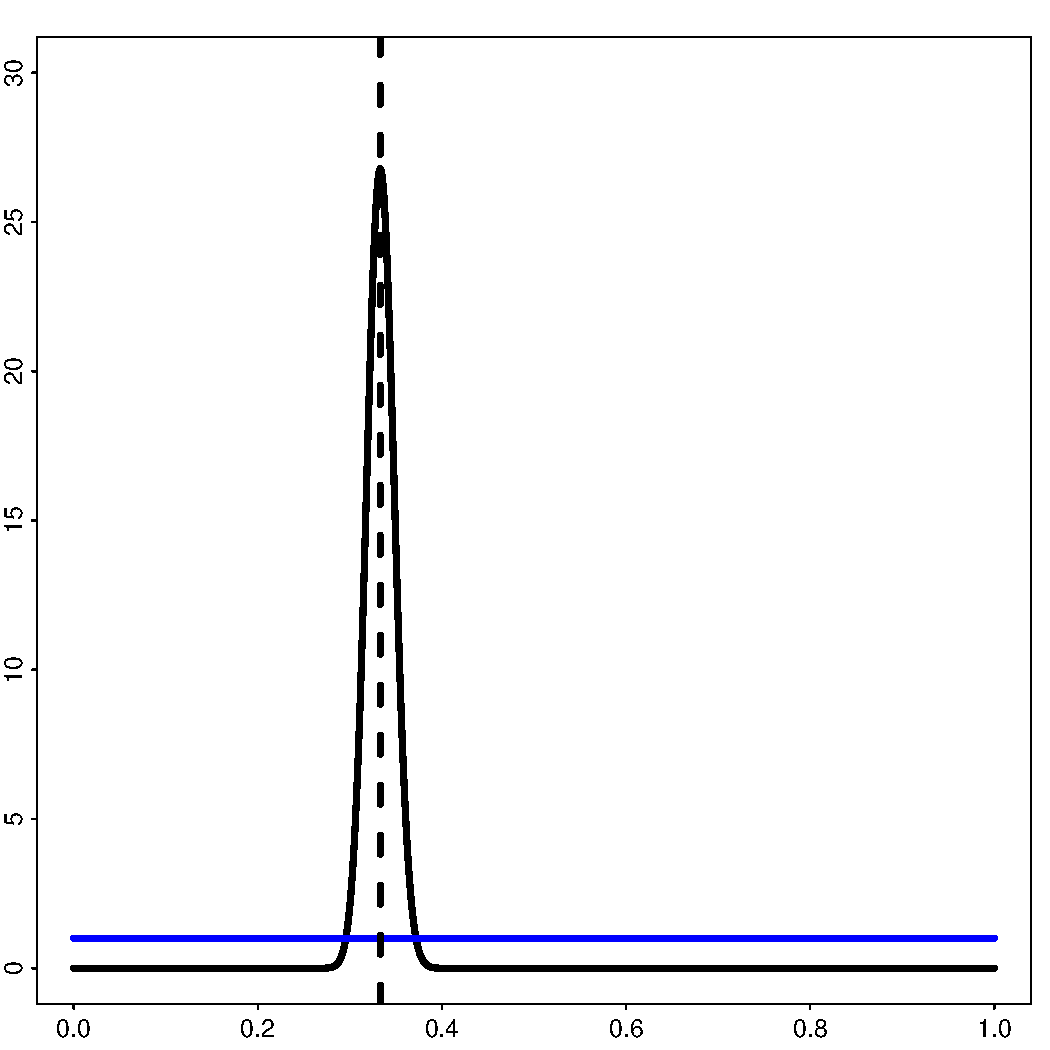
\includegraphics[width=.3\textwidth, height=.25\textheight]{../figs/beta-binomial-a1-b1-n1000-p33} 
  \end{tabular}
}

%====================================================================
\frame{ \frametitle{Back to logistic regression}

  \paragraph{Model}
  \begin{itemize}
   \item Prior: all coefficient $\theta_j$ independent:
   $$
   \theta_j \sim \Ncal(0, 100)
   $$
   \item Likelihood: all patients independent, {\sl conditionally} on $\thetabf$:
   $$
   \Pr\{Y_i = 1 \gv \thetabf\} = e^{\xbf_i^\intercal \thetabf} \left/ \left( 1 + e^{\xbf_i^\intercal \thetabf} \right) \right. 
   $$
  \end{itemize}
  
  \paragraph{Inference:}
  $$
  \thetabf \gv \Ybf \sim \; ? 
  $$
  
  \bigskip
  (see later. For sure: $p(\thetabf \gv \Ybf) \neq \Ncal(\cdot, \cdot)$).
}

%====================================================================
\frame{ \frametitle{Bayesian inference}

  \paragraph{Output:} 
  $$
  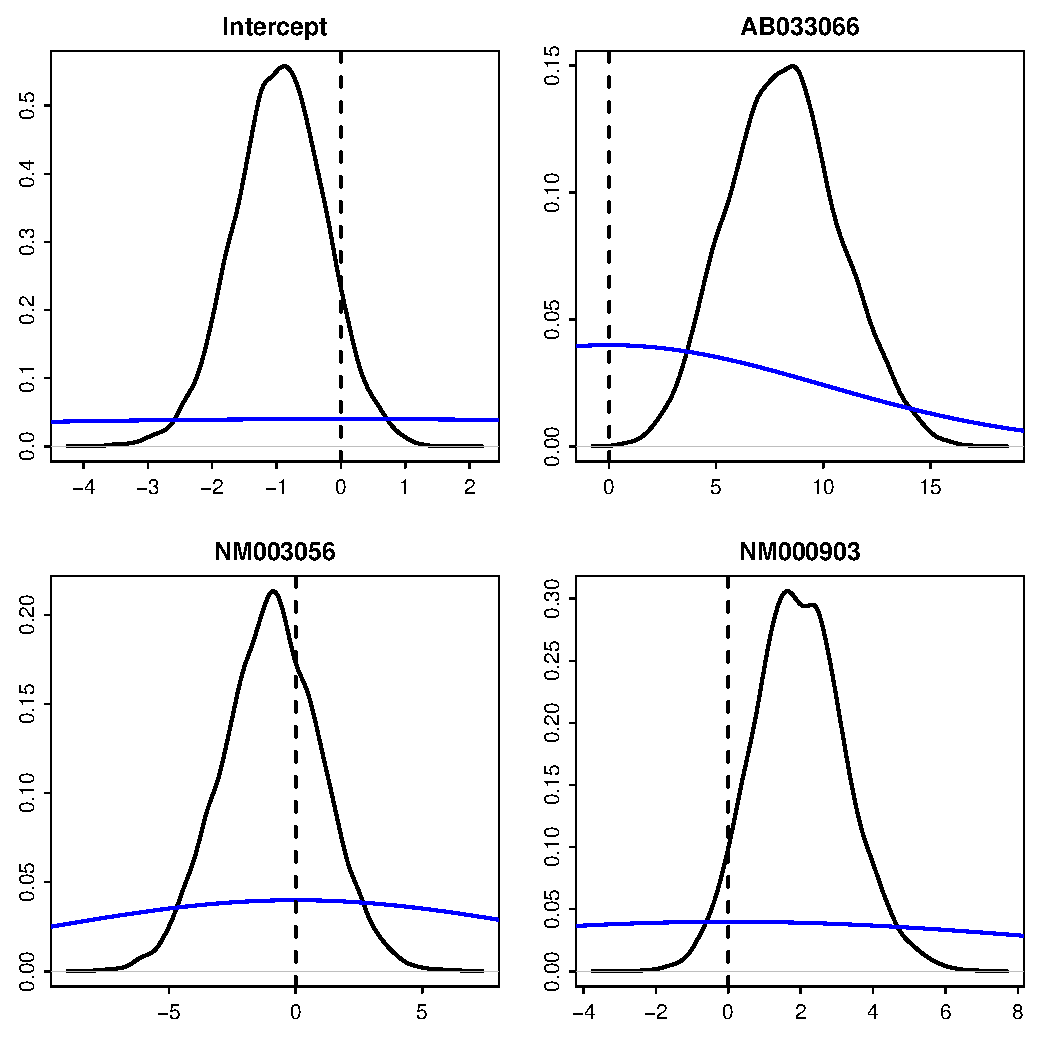
\includegraphics[width=.8\textwidth, height=.8\textheight]{\figfig/posterior-density}
  $$
}

%====================================================================
\frame{ \frametitle{No test (and no estimator)} 

  \paragraph{Frequentist hypothesis:}
  $$
  H_0 = \{\theta = 0\}
  $$
  \ra meaningless when $\theta$ is random: $P(H_0 \gv \Ybf) = 0$
  
  \pause \bigskip \bigskip
  \paragraph{Bayesian assessment:}
  $$
  CI_{1 - \alpha}(\theta \gv \Ybf) \ni 0 \; ?
  $$

  \pause \bigskip \bigskip
  \paragraph{Parameter estimate.} For the same reason:
  $$
  \widehat{\theta} \text{ can no be an estimate of } \theta
  $$
  (because $\theta$ is random).
  
}

%====================================================================
\subsection{Some typical uses of Bayesian inference}
\frame{\frametitle{Outline} \tableofcontents[currentsubsection]}
%====================================================================
\frame{ \frametitle{Posterior distribution and confidence intervals} \label{sec:CI}

  \paragraph{Parameter 'estimate'.}
  \begin{align*}
   \text{posterior mean:} \qquad \widehat{\theta}_j & = \Esp(\theta_j \gv \Ybf)  \\
   \text{posterior mode:} \qquad \widehat{\theta}_j & = \arg\max _{\theta_j} \; p(\theta_j \gv \Ybf)
  \end{align*}

  \bigskip
  \paragraph{Credibility interval (CI).} With level $1 - \alpha$ (e.g. 95\%):
  $$
  CI_{1-\alpha}(\theta_j \gv \Ybf) = [\theta_j^\ell; \theta_j^u]:
  \qquad 
  \Pr\{\theta_j^\ell < \theta_j < \theta_j^u \gv \Ybf\} = 1-\alpha
  $$

  \bigskip \pause
  \paragraph{Example.} \appref{app:CIcontrast}
  \begin{center} {\tt \begin{tabular}{lrrrcr}
    & post.mean  & post.mode  & lower.CI  & upper.CI \\ 
    \hline 
    Intercept  & -0.9298079  & -0.8838218  & -2.457669  & 0.5376564 \\ 
    AB033066  & 8.656539  & 8.497985  & 3.646142  & 13.98029 \\ 
    NM003056  & -0.8669479  & -0.5323168  & -4.919099  & 3.084982 \\ 
    NM000903  & 2.088584  & 1.852784  & -0.4736828  & 4.838164 
    \end{tabular} } \end{center}
}

%====================================================================
\frame{ \frametitle{Accounting for uncertainty}

  \paragraph{Question:} What is the probability for patient 0 (with profile $\xbf_0$) to be sick?

  \bigskip \bigskip 
  \paragraph{Model answer:}
  $$
  \Pr\{Y_0 = 1 \gv \thetabf\} = e^{\xbf_0^\intercal \thetabf} \left/ \left( 1 + e^{\xbf_0^\intercal \thetabf} \right) \right. 
  $$
  but $\thetabf$ is unknown (and random).
  
  \bigskip \bigskip 
  \paragraph{Bayesian answer:} {\sl posterior predictive} probability
  $$
  \Pr\{Y_0 = 1 \gv \Ybf\} = \int \Pr\{Y_0 = 1 \gv \thetabf\} p(\thetabf \gv \Ybf) \d \thetabf
  $$
}

%====================================================================
\frame{ \frametitle{Model comparison (1/2)}

  \paragraph{Problem.} Which model fits the data better:
  \begin{align*}
   M_0 &: \text{none of the genes has an effect, i.e. $\thetabf = (\theta_0, 0, \dots, 0)$} \\
   M_1 &: \text{only the fist gene has an effect, i.e. $\thetabf = (\theta_0, \theta_1, 0, \dots, 0)$} \\
   & \dots
   \\
   M_p &: \text{all genes have an effect, i.e. $\thetabf = (\theta_0, \theta_1, \dots,  \theta_p)$} 
   \end{align*}

   \bigskip \bigskip 
   \paragraph{Bayesian model comparison.} For each model $M \in \Mcal =\{M_0, \dots, M_p\}$, evaluate
   $$
   p(M \gv \Ybf)
   $$
}
   
%====================================================================
\frame{ \frametitle{Model comparison (2/2)}

  \paragraph{Ingredients:}
  \begin{itemize}
   \item Prior on the models: $p(M)$, e.g.
   $$
   p(M) = \cst \qquad \text{(uniform prior)}
   $$
   \item Conditional prior on the parameters: $\pi(\thetabf \gv M)$, e.g.
   $$
   \theta_j \gv M_k \; \left\{ 
   \begin{array} {rll}
   \sim & \Ncal(0, 100) & \text{if $ j \leq k$} \\
   = & 0 & \text{otherwise}
   \end{array}\right.
   $$
  \end{itemize}

  \bigskip \pause
  \paragraph{Recipe:}
  \begin{itemize}
  \item Evaluate the marginal likelihood of the data for each model $M$:
  $$
  p(\Ybf \gv M) = \int \ell(\Ybf \gv \thetabf) \pi(\thetabf \gv M) \d \thetabf
  $$
  \item \pause Evaluate the $p(M_k \gv \Ybf)$ using Bayes rule
  $$
  p(M_k \gv \Ybf) = \frac{p(M_k) p(\Ybf \gv M_k)}{p(\Ybf)} = \frac{p(M_k) p(\Ybf \gv M_k)}{\sum_{k'} p(M_{k'}) p(\Ybf \gv M_{k'})}
  $$
  \end{itemize}
 }

%====================================================================
\frame{ \frametitle{Model averaging (uncertainty on models)}

  \paragraph{Question:} Probability for patient 0 to be sick?
  
  \bigskip \bigskip \pause
  \paragraph{Model selection.}
  \begin{itemize}
   \item Select the 'best' model $\widehat{M}$, i.e. with largest posterior $p(M \gv \Ybf)$
   \item Compute
   $$
  \Pr\{Y_0 = 1 \gv \Ybf, \widehat{M} \} = \int \Pr\{Y_0 = 1 \gv \thetabf\} p(\thetabf \gv \Ybf, \widehat{M}) \d \thetabf
   $$
  \end{itemize}

  \bigskip \pause
  \paragraph{Model averaging.}
  \begin{itemize}
   \item Keep all models
   \item Compute
   $$
   \Pr\{Y_0 = 1 \gv \Ybf\} = \sum_M \Pr\{Y_0 = 1 \gv \Ybf, M\} p(M \gv \Ybf)
   $$
  \end{itemize}
}

%====================================================================
\frame{ \frametitle{Model averaging: Illustration}

  \paragraph{Aim:} Probability \emphase{$p_0$} to be sick a patient with gene expression profile
  $$
  \xbf_0 = (0.178, 0.116, \dots, 0.076, -0.231)
  $$
  
  \paragraph{Results} for models $M_1, \dots, M_d$:
  $$
  \begin{tabular}{lrrr}
  Model & $p(M \gv \Ybf)$ & $\Esp(p_0 \gv \Ybf, M)$ & $\sqrt{\Var}(p_0 \gv \Ybf, M)$ \\ 
  \hline 
  $M_{1}$  & 1e-04  & 0.494  & 0.028 \\
  $M_{2}$  & 7e-04  & 0.611  & 0.097 \\ 
  $M_{3}$  & 5e-04  & 0.627  & 0.106 \\ 
  \dots & & & \\
  $M_{14}$  & 0.1436  & 0.242  & 0.18 \\
  $M_{15}$  & 0.2859  & 0.203  & 0.168 \\ 
  $M_{16}$  & 0.2726  & 0.195  & 0.168 \\
  \hline \\ \hline
  Averaging & & $\Esp(p_0 \gv \Ybf)$ & $\sqrt{\Var}(p_0 \gv \Ybf)$ \\ 
  \hline 
  & & 0.249 & 0.198 
  \end{tabular}
  $$

  
}

%====================================================================
\frame{ \frametitle{Transfer of uncertainty from one experience to another}

  \paragraph{Combining samples.} Consider two independent but similar datasets $\Ybf_1$ and $\Ybf_2$.
  
  \bigskip
  Simple algebra gives:
  $$
  p(\thetabf \gv \Ybf_1, \Ybf_2) 
  = \frac{p(\thetabf \gv \Ybf_1) p(\Ybf_2 \gv \thetabf, \Ybf_1) }{p(\Ybf_2 \gv \Ybf_1)}
  $$
  
  \bigskip \pause
  \paragraph{In practice:}
  \begin{enumerate}
  \item Perform inference using $\Ybf_1$ to get $p(\thetabf \gv \Ybf_1)$ from prior $\pi(\thetabf)$
  \item Then perform inference using $\Ybf_2$ to get $p(\thetabf \gv \Ybf_1, \Ybf_2)$ \emphase{using  $p(\thetabf \gv \Ybf_1)$ as a prior}
  \end{enumerate}
}

%====================================================================
\frame{ \frametitle{Combining experiments}

  \paragraph{Output:} $n_1 = n_2 = 39$
  $$
  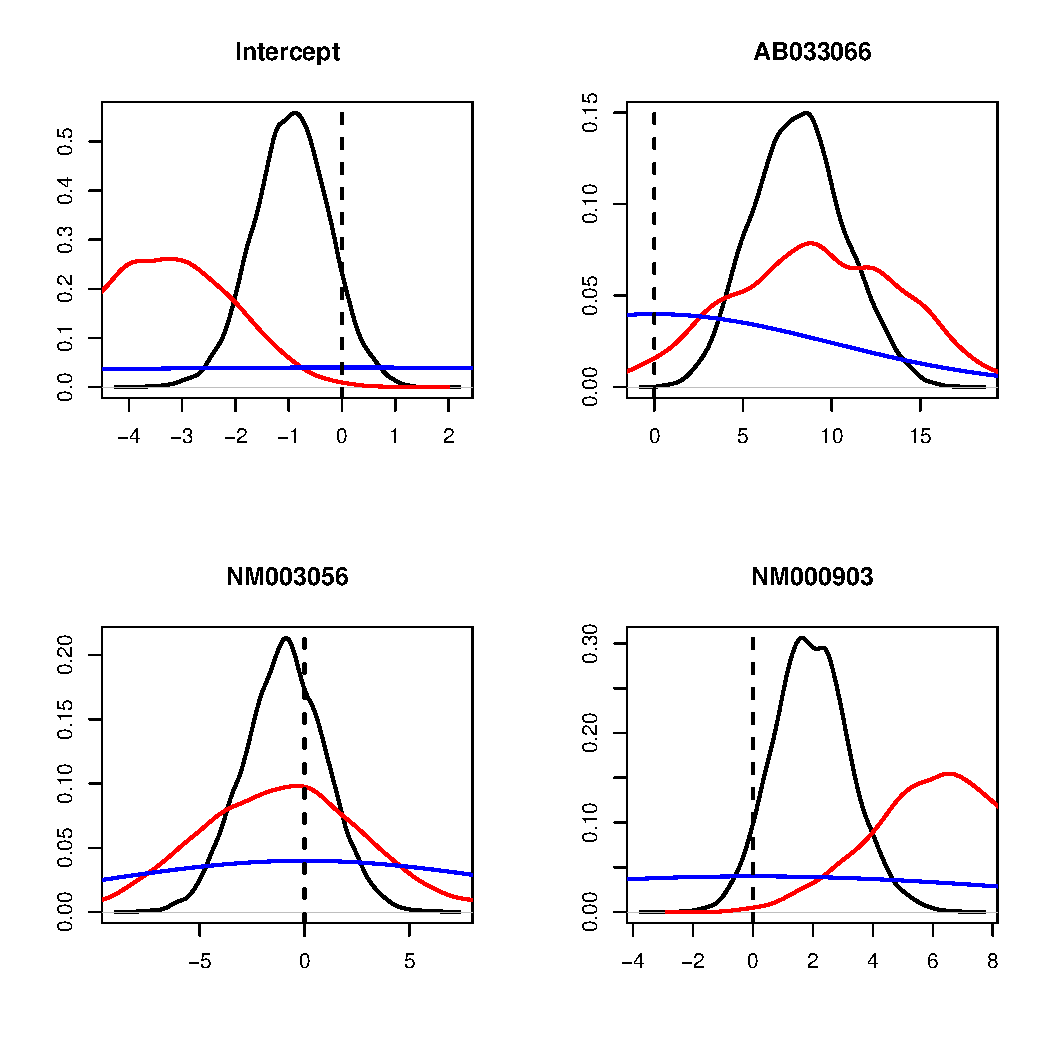
\includegraphics[width=.8\textwidth, height=.8\textheight]{\figfig/posterior-combine}
  $$
}



%====================================================================
\section{Evaluating the posterior distribution: Monte-Carlo} \label{sec:MCMC}
\frame{\frametitle{Outline} \tableofcontents[currentsection]}
%====================================================================
\frame{ \frametitle{Posterior distribution}

  \paragraph{Aim:} Evaluate
  $$
  E[f(\thetabf) | \Ybf]
  $$
  \begin{itemize}
   \item Posterior mean: $f(\thetabf) = \theta_j$
   \item Credibility interval: $f(\thetabf) = \Ibb\{\theta^\ell_j < \theta_j < \theta^u_j\}$
   \item Posterior variance: $f(\thetabf) = \theta_j^2$ \qquad (+ posterior mean)
   \item Posterior covariance: $f(\thetabf) = \theta_j \theta_k$ \qquad (+ posterior means)
  \end{itemize}

  \bigskip \bigskip \pause
  \paragraph{Main problem:} evaluate
  $$
  p(\thetabf \gv \Ybf) = \frac{\pi(\thetabf) \bf \ell(\Ybf \gv \thetabf)}{p(\Ybf)}
  $$
  which requires to evaluate
  $$
  p(\Ybf) = \int \underset{prior}{\underbrace{\pi(\thetabf)}} \; \underset{likelihood}{\underbrace{\ell(\Ybf \gv \thetabf)}} \d \thetabf
  $$
}

%====================================================================
\subsection{Conjugate priors}
\frame{\frametitle{Outline} \tableofcontents[currentsubsection]}
%====================================================================
\frame{ \frametitle{Nice case: Conjugate priors}

  \paragraph{Example: Bernoulli}\footnote{\#\ref{slide:prior}: from top to bottom, $(a, b) = (1, 10), (5, 5), (1, 1)$}
  \begin{description}
   \item[Prior:] $\theta =$ probability to carry a disease. 
   $$
   \theta \sim \Beta(a, b), 
   \qquad 
   \pi(\theta) \propto \theta^{a-1} (1-\theta)^{b-1}
   $$ \pause
   \item[Likelihood:] $Y_i = 1$ if disease, $0$ otherwise. $S =$ number of carriers
   $$
   Y_i \gv \theta \sim \Bcal(\theta), 
   \qquad 
   \ell(\Ybf \gv \theta) = \prod_i \theta^{Y_i} (1-\theta)^{1-Y_i} = \theta^{S} (1-\theta)^{n-S}
   $$ \pause
   \item[Posterior:]
   $$
   p(\theta \gv \Ybf) \propto \pi(\theta) \ell(\Ybf \gv \theta) = \theta^{a+S-1} (1-\theta)^{b+n-S-1}
   $$
   which means that
   $$
   \theta \gv \Ybf \sim \Beta(a+S, b+n-S)
   $$
  \end{description}
}

%====================================================================
\frame{ \frametitle{Conjugate priors: Discrete distributions}

  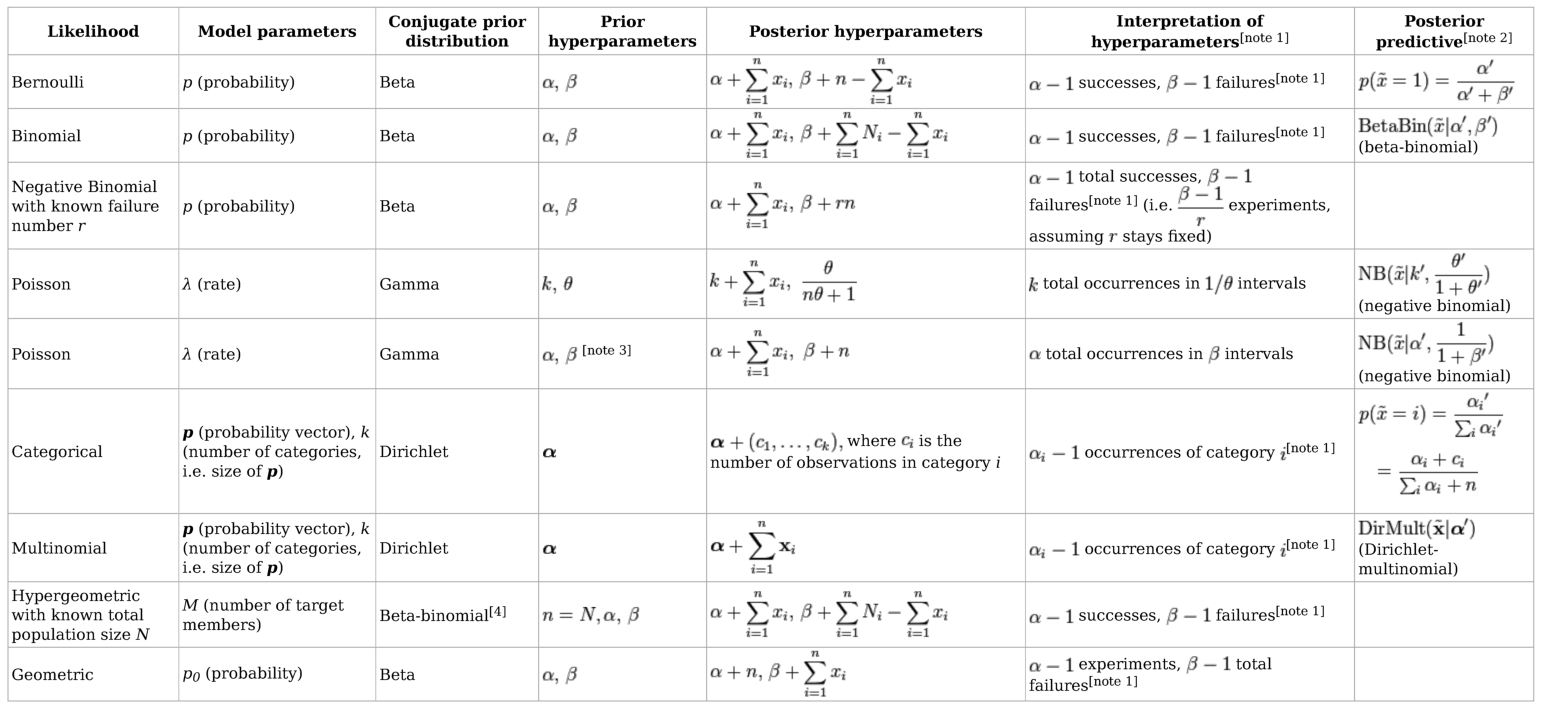
\includegraphics[width=1\textwidth]{../figs/WikipediaConjugatePrior-Discrete}

  \footnotesize{\url{en.wikipedia.org/wiki/Conjugate_prior}}
}

%====================================================================
\frame{ \frametitle{Conjugate priors: Continuous distributions}

  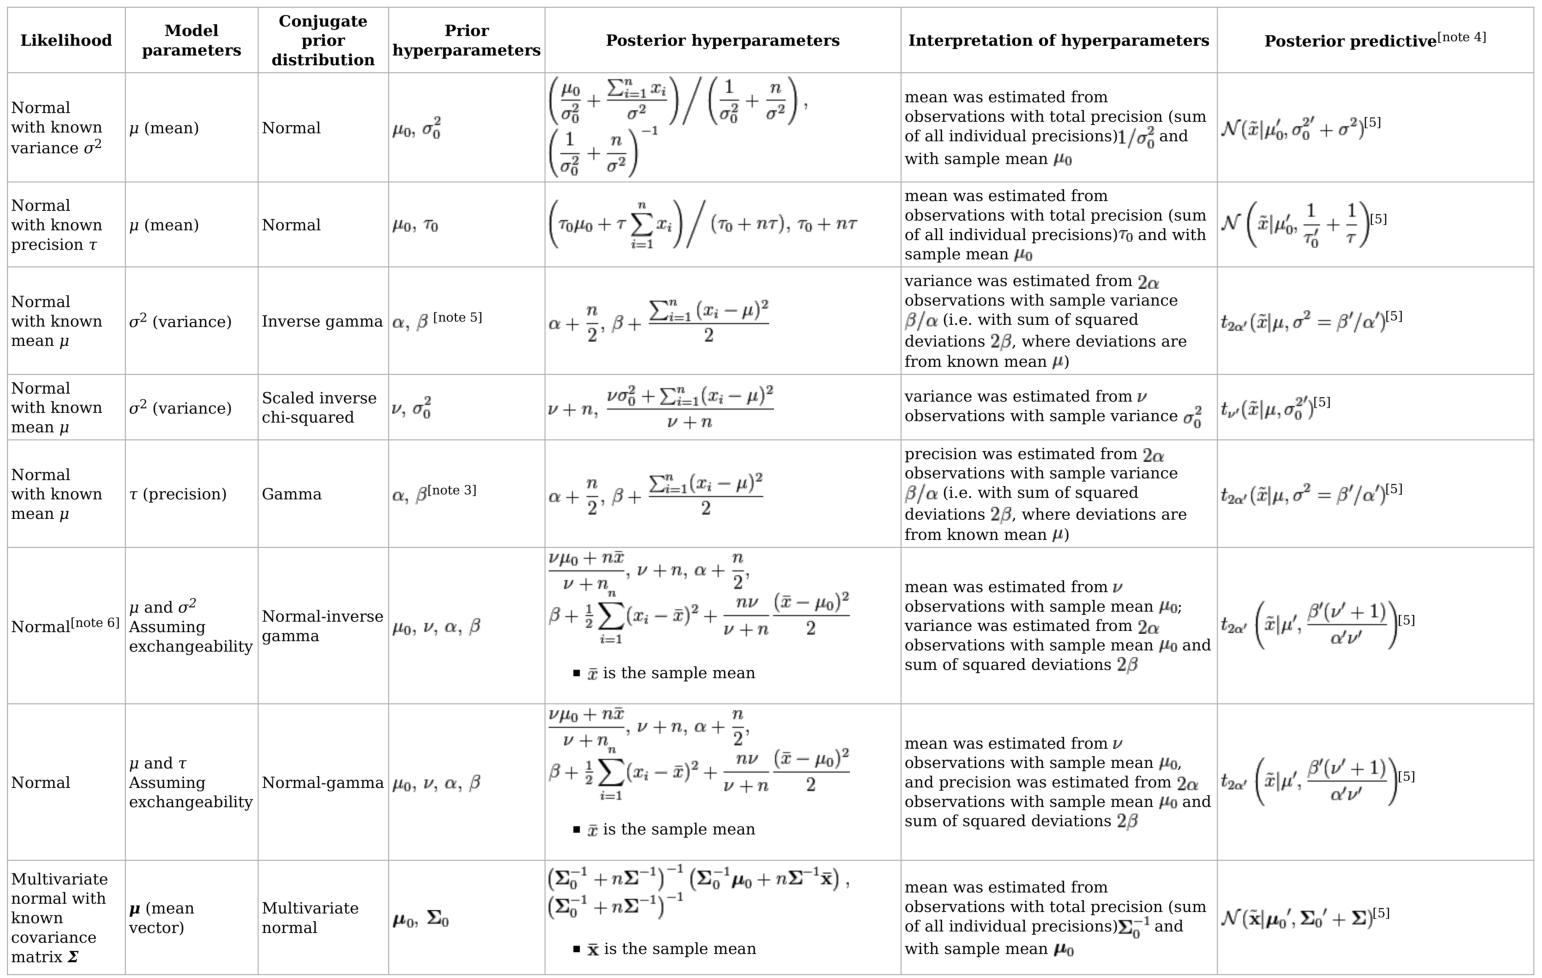
\includegraphics[width=1\textwidth]{../figs/WikipediaConjugatePrior-Continuous}

  \footnotesize{\url{en.wikipedia.org/wiki/Conjugate_prior}}
}

%====================================================================
\subsection{Monte Carlo integration}
\frame{\frametitle{Outline} \tableofcontents[currentsubsection]}
%====================================================================
\frame{ \frametitle{Computing integrals}

  \paragraph{General case:} $p(\thetabf \gv \Ybf)$ has no close form
  
  \bigskip 
  \paragraph{Goal:} compute
  $$
  \Esp(f(\thetabf) \gv \Ybf) 
  = \int f(\thetabf) p(\thetabf \gv \Ybf) \d \thetabf
  = \left. \int f(\thetabf) \pi(\thetabf) \; \ell(\Ybf \gv \thetabf) \d \thetabf \right/ p(\Ybf) 
  $$
  where
  $$
  p(\Ybf) = \int \pi(\thetabf) \; \ell(\Ybf \gv \thetabf) \d \thetabf 
  $$
  
  \bigskip \bigskip \pause
  We need to evaluate integrals of the form
  $$
  \int [\cdots] \; \emphase{\pi(\thetabf) \; \ell(\Ybf \gv \thetabf)} \d \thetabf 
  $$
}

%====================================================================
\frame{ \frametitle{Monte Carlo}

  \paragraph{Principle.} To evaluate
  $$
  \Esp_q[f(\thetabf)] = \int f(\thetabf) \emphase{q(\thetabf)} \d \thetabf
  $$
  \begin{enumerate}
   \item \pause sample 
   $$
   (\thetabf^1, \dots, \thetabf^B) \text{ iid } \sim q
   $$
   \item \pause compute
   $$
   \widehat{\Esp}_q[f(\thetabf)] = \frac1B \sum_b f(\thetabf^b)
   $$
  \end{enumerate}
  \pause \ra unbiased estimate of $\Esp_q[f(\thetabf)]$ with variance $\propto 1/ B$. \appref{app:MCillustration}
  
  \bigskip \bigskip \pause
  \paragraph{In practice:} 
  \begin{itemize}
   \item Works fine to evaluate $\Esp[f(\thetabf)]$, taking $q(\thetabf) = \pi(\thetabf)$
   $$
   \widehat{\Esp}_{\Ncal(0, 10)}\left[e^\theta\right] = \text{\tt mean(exp(rnorm(B, mean=0, sd=sqrt(10))))}
   $$\pause
   \item Useless to evaluate $\Esp[f(\thetabf) | \Ybf]$ as we do not know how to sample from $q(\thetabf) = p(\thetabf \gv \Ybf)$
  \end{itemize}
}

%===================================================================
\frame{ \frametitle{Importance Sampling (IS)}

  \paragraph{Main trick = weighting particles.} \pause To evaluate $\Esp[f(\thetabf)]$, write it as
  \begin{align*}
  \Esp_q[f(\thetabf)] 
  = \int f(\thetabf) q(\thetabf) \d \thetabf 
  = \int f(\thetabf) \frac{q(\thetabf)}{\emphase{q'(\thetabf)}} \emphase{q'(\thetabf)} \d \thetabf 
  \end{align*}
  for some \emphase{proposal} $q' \gg q$, from which you {\sl know how to sample}, then
  \begin{enumerate}
   \item \pause sample
   $$
   (\thetabf^1, \dots, \thetabf^B) \text{ iid } \sim \emphase{q'}(\thetabf),
   $$
   \item \pause compute the weights
   $$
   W(\thetabf^b) = q(\thetabf^b) / q'(\thetabf^b), 
   $$
   \item \pause and compute
   $$
   \widehat{\Esp}[f(\thetabf)] = \frac1B \sum_b W(\thetabf^b) f(\thetabf^b)
   $$
  \end{enumerate}
  \pause \ra unbiased estimate of $\Esp[f(\thetabf)]$ with variance $\propto \sum_b W(\theta^b)^2 / B$.

}  

%===================================================================
\frame{ \frametitle{Importance Sampling (a picture)}

  \begin{tabular}{cc}
    \begin{tabular}{p{.3\textwidth}}
	 \onslide+<4>{
	   Efficiency of sampling:
	   $$
	   ESS = \overline{W}^2 / \overline{W^2}
	   $$

	   \bigskip
	   $q' = q$
	   $$
	   \Rightarrow \quad ESS = 1
	   $$
	   }
    \end{tabular}
    & 
%     \hspace{-.\textwidth}
    \begin{tabular}{p{.5\textwidth}}
	 \begin{overprint}
	 \onslide<1>
	 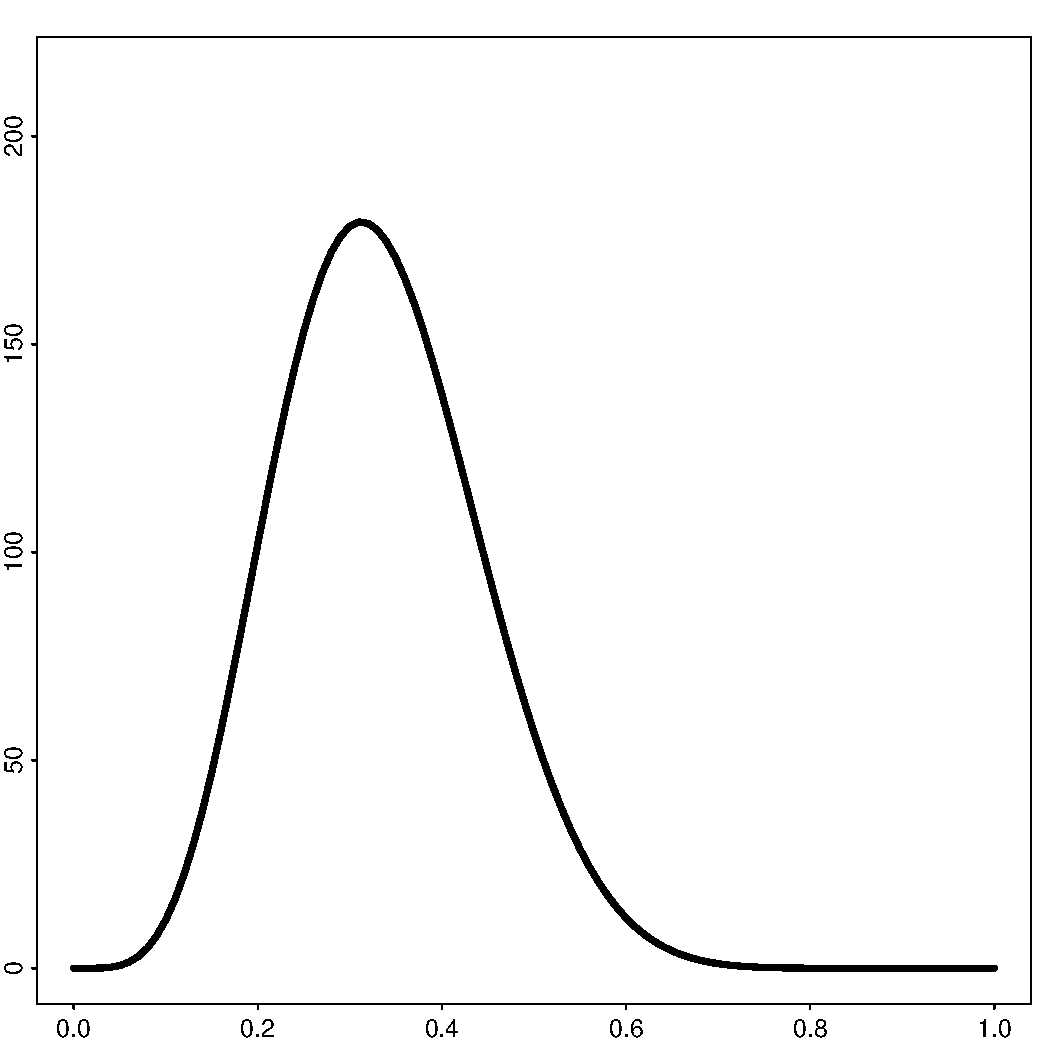
\includegraphics[height=.7\textheight]{../figs/ImportanceSampling-1}
	 \onslide<2>
	 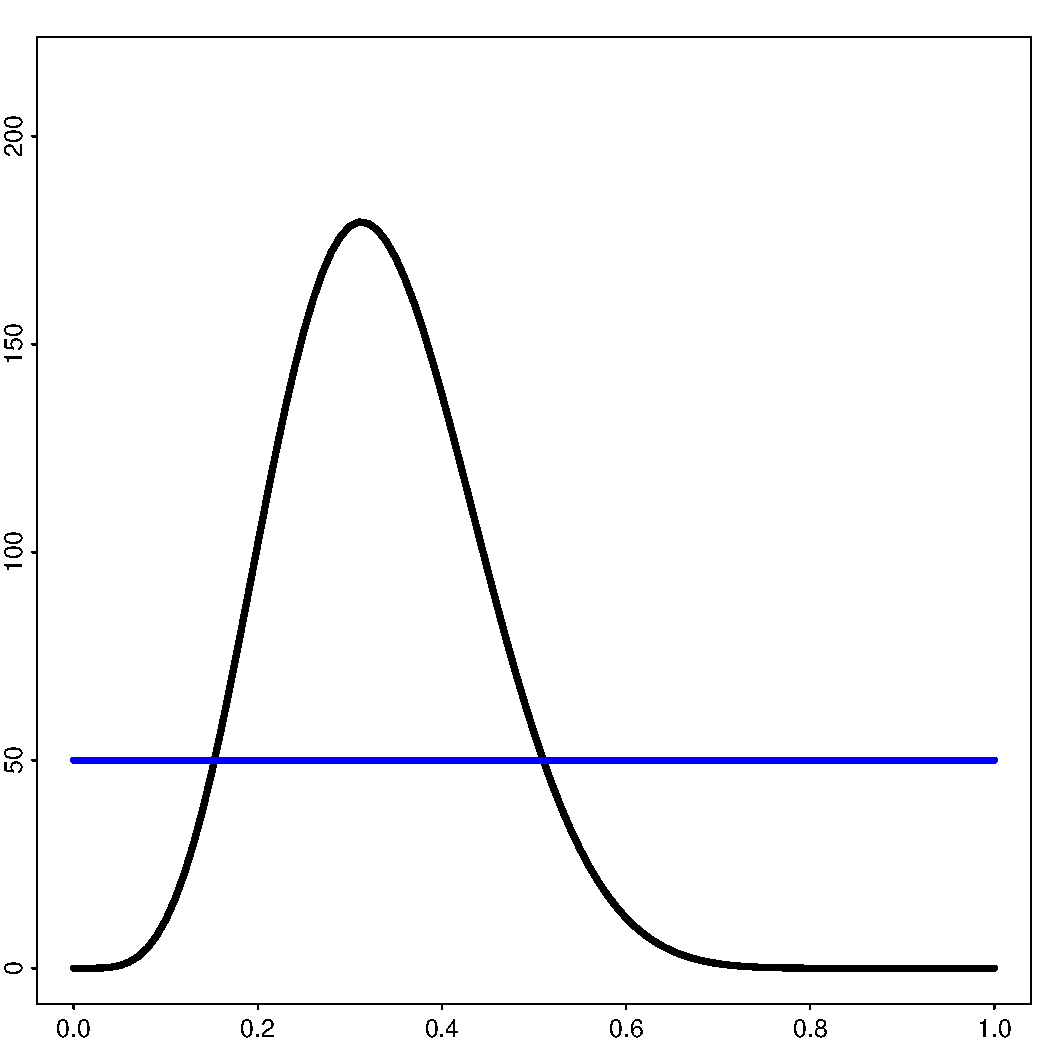
\includegraphics[height=.7\textheight]{../figs/ImportanceSampling-2}
	 \onslide<3>
	 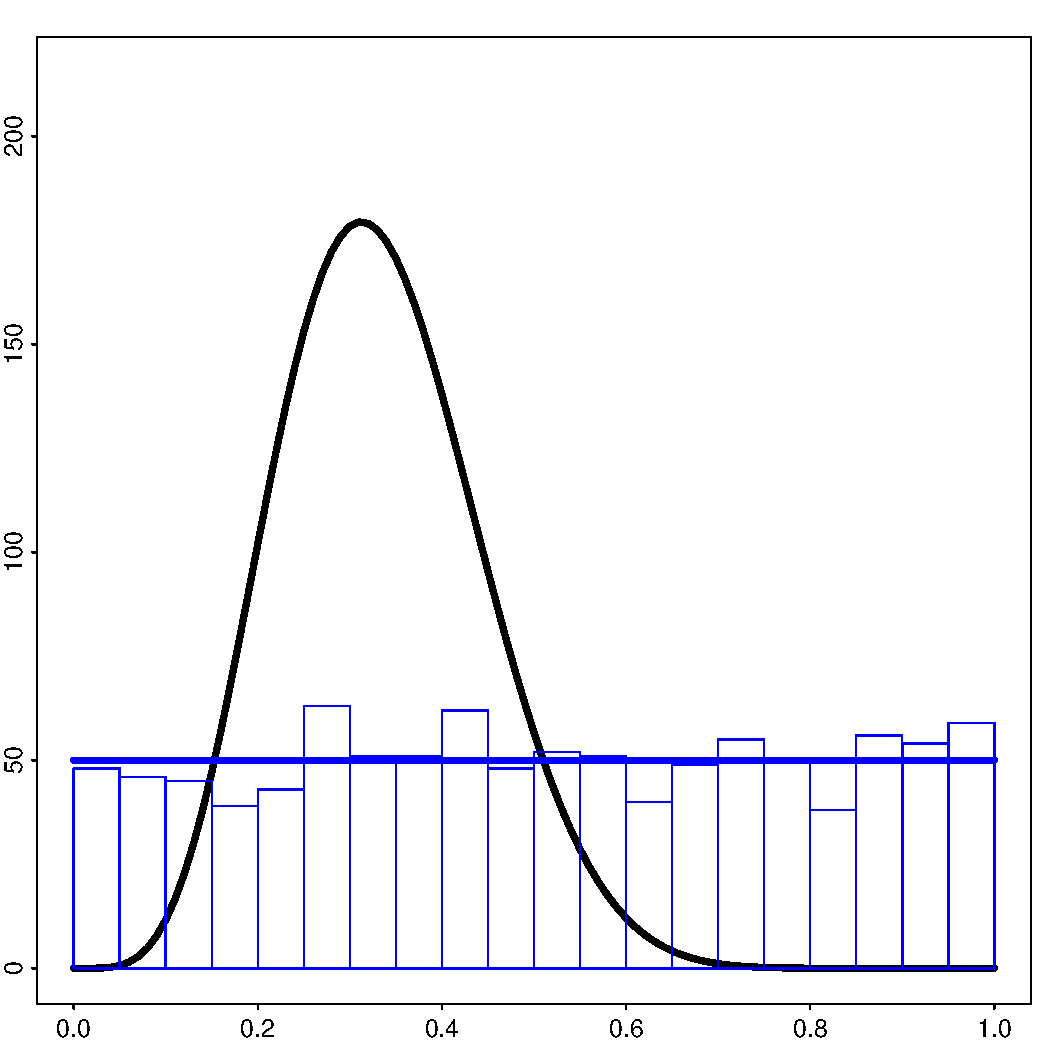
\includegraphics[height=.7\textheight]{../figs/ImportanceSampling-3}
	 \onslide<4>
	 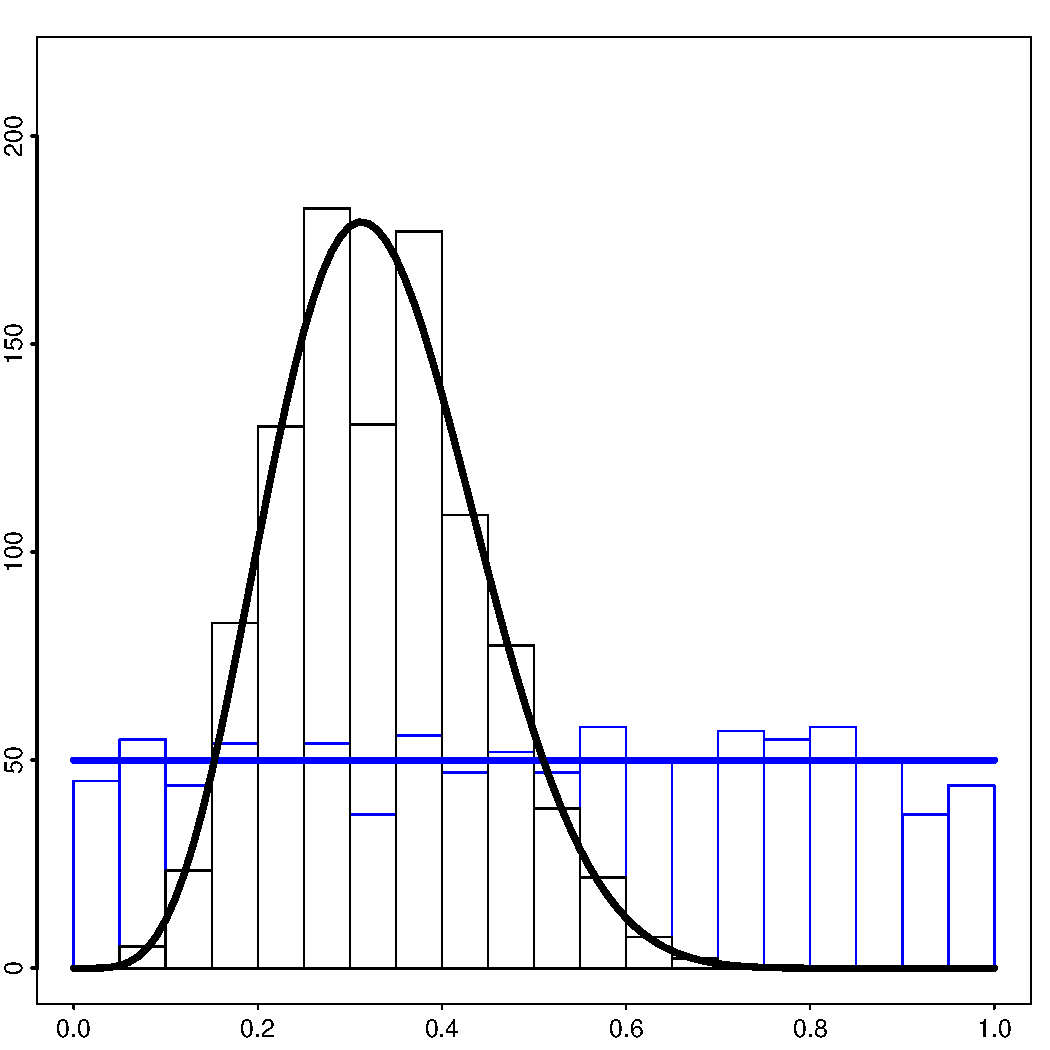
\includegraphics[height=.7\textheight]{../figs/ImportanceSampling-4}
	 \end{overprint}
    \end{tabular}
  \end{tabular}

}  


%===================================================================
\frame{ \frametitle{Importance Sampling: Importance of the proposal}

%   \begin{center}
%   \begin{tabular}{cc}
%     \begin{tabular}{c}
%     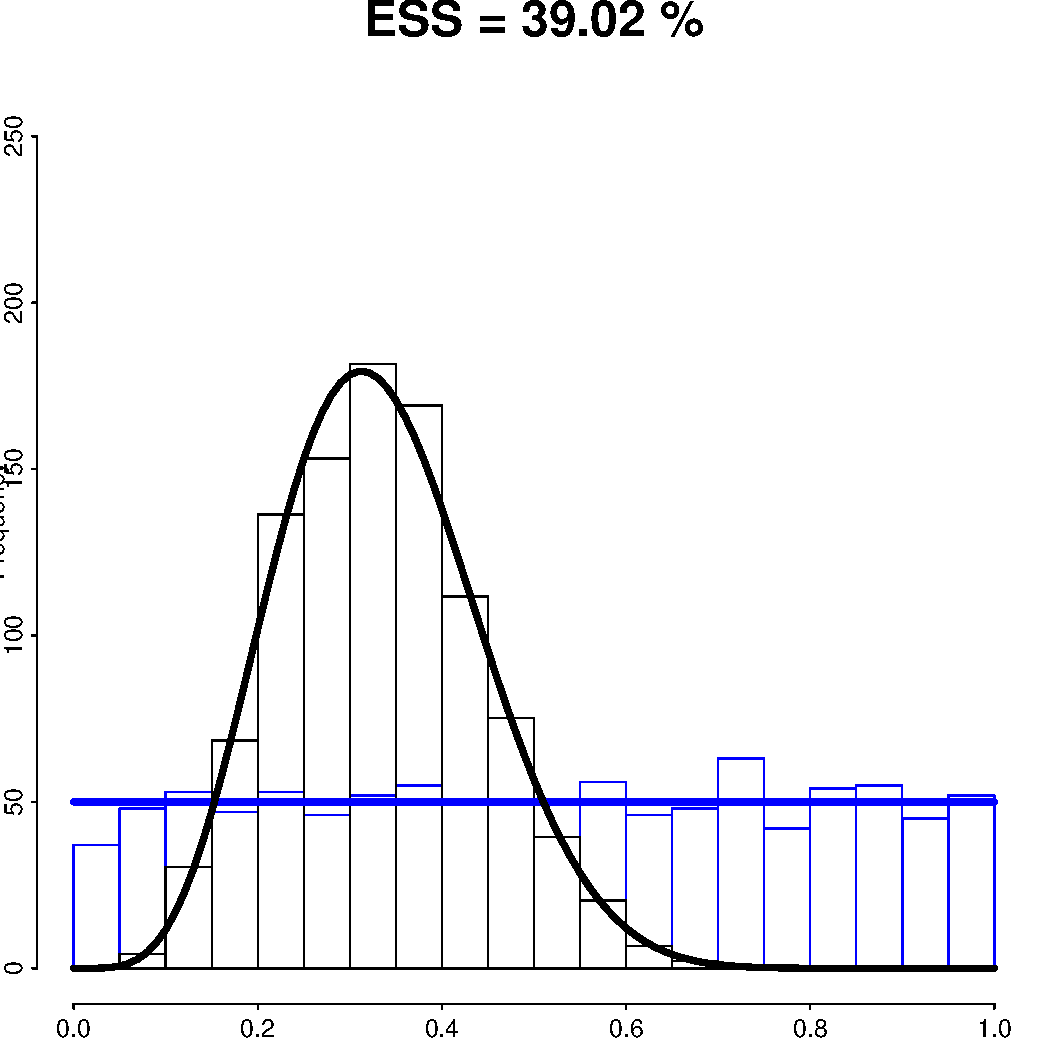
\includegraphics[height=.4\textheight]{../figs/ImportanceSampling-Beta-a06-b012-a1-b1-seed4} 
%     \end{tabular}
%     & 
%     \begin{tabular}{c}
%     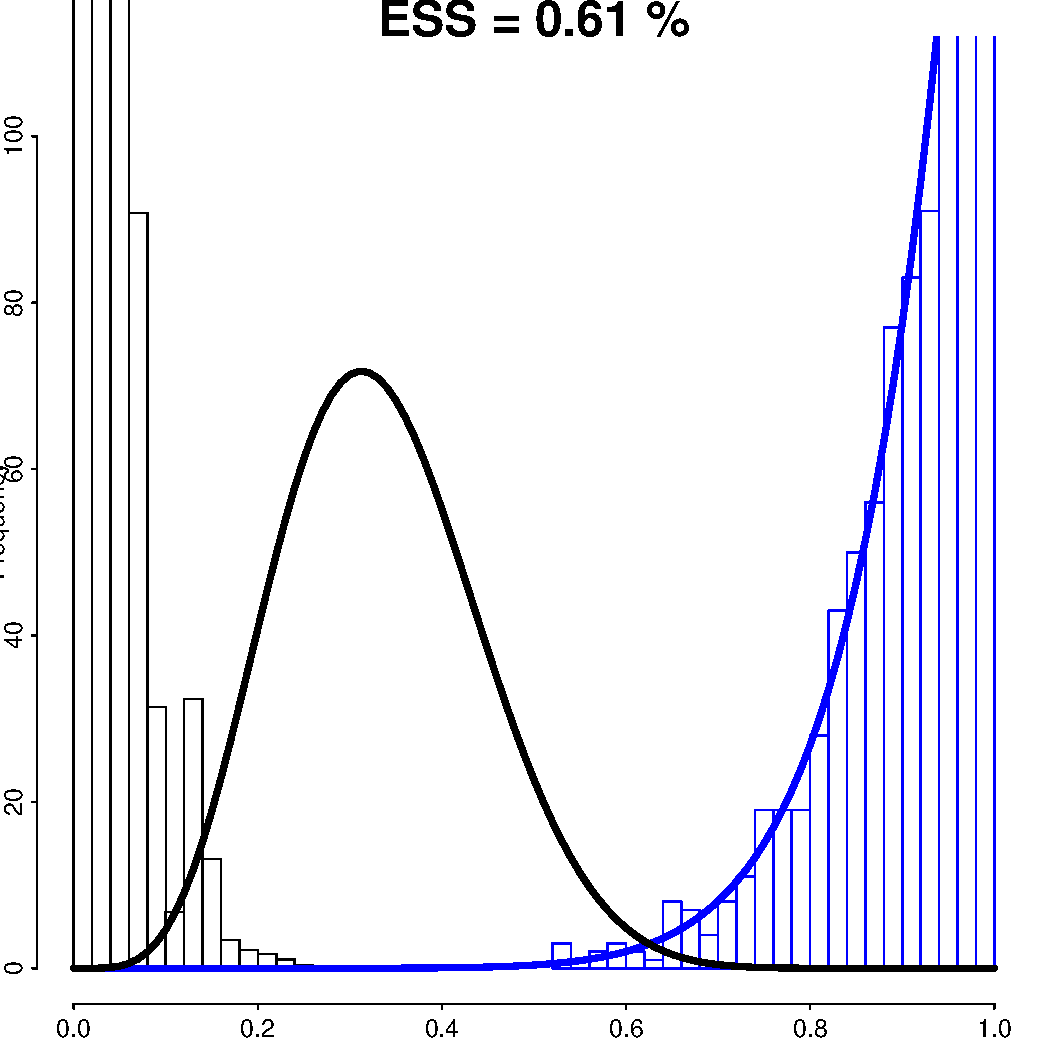
\includegraphics[height=.4\textheight]{../figs/ImportanceSampling-Beta-a06-b012-a10-b1-seed4} 
%     \end{tabular}
%     \\ \\
%     \begin{tabular}{c}
%     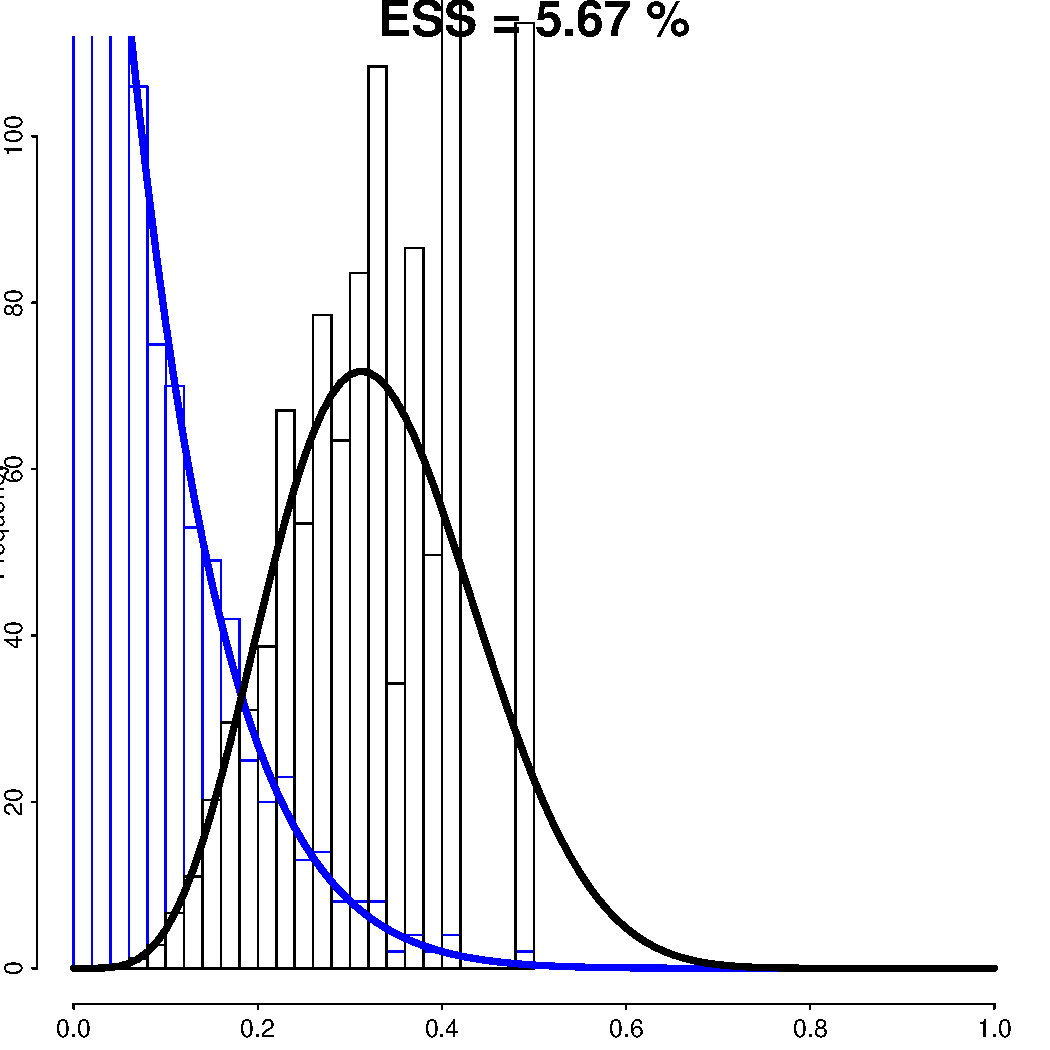
\includegraphics[height=.4\textheight]{../figs/ImportanceSampling-Beta-a06-b012-a1-b10-seed4} 
%     \end{tabular}
%     & 
%     \begin{tabular}{c}
%     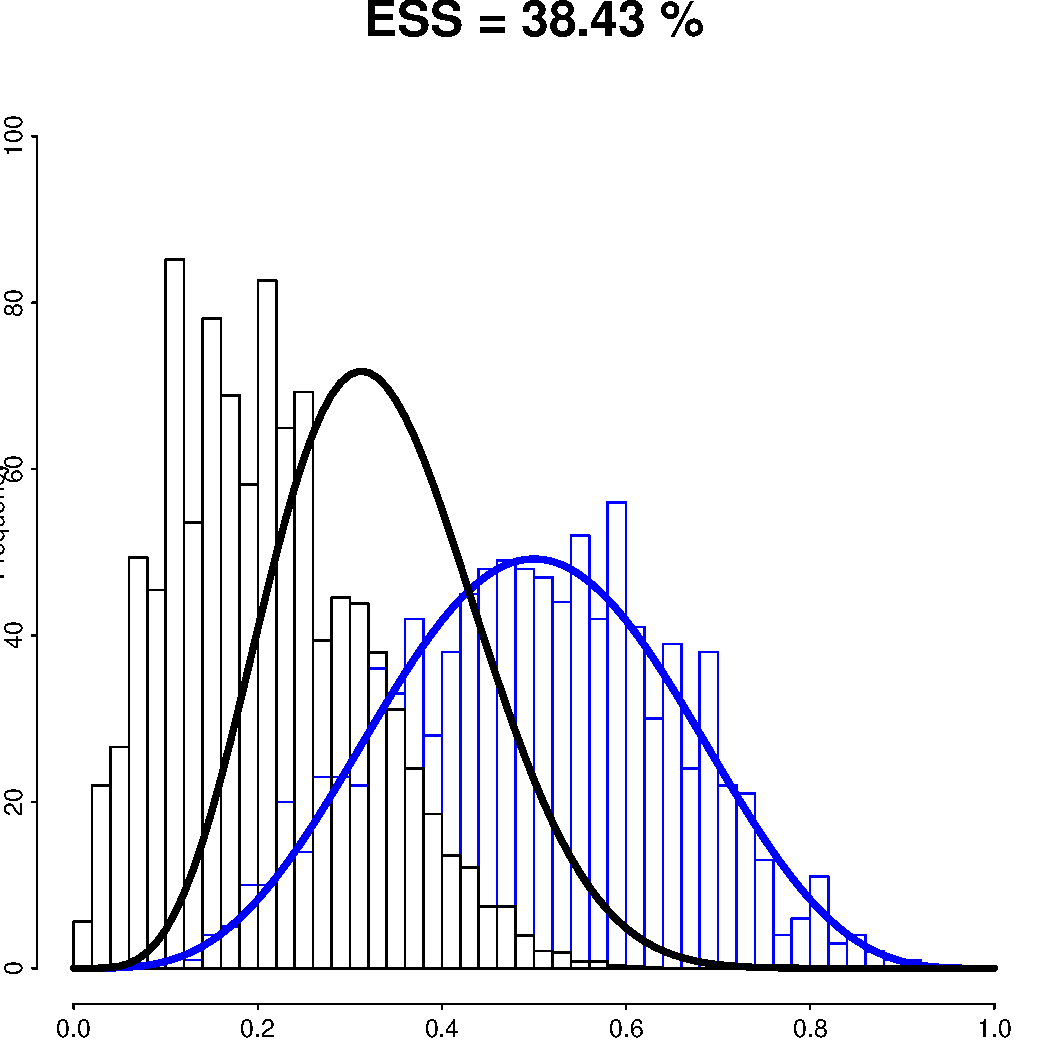
\includegraphics[height=.4\textheight]{../figs/ImportanceSampling-Beta-a06-b012-a5-b5-seed4} 
%     \end{tabular}
%   \end{tabular}
%   \end{center}
%  }  
% 
% %===================================================================
% \frame{ \frametitle{Importance of the proposal: another draw}

  \begin{center}
  \begin{tabular}{cc}
    \begin{tabular}{c}
    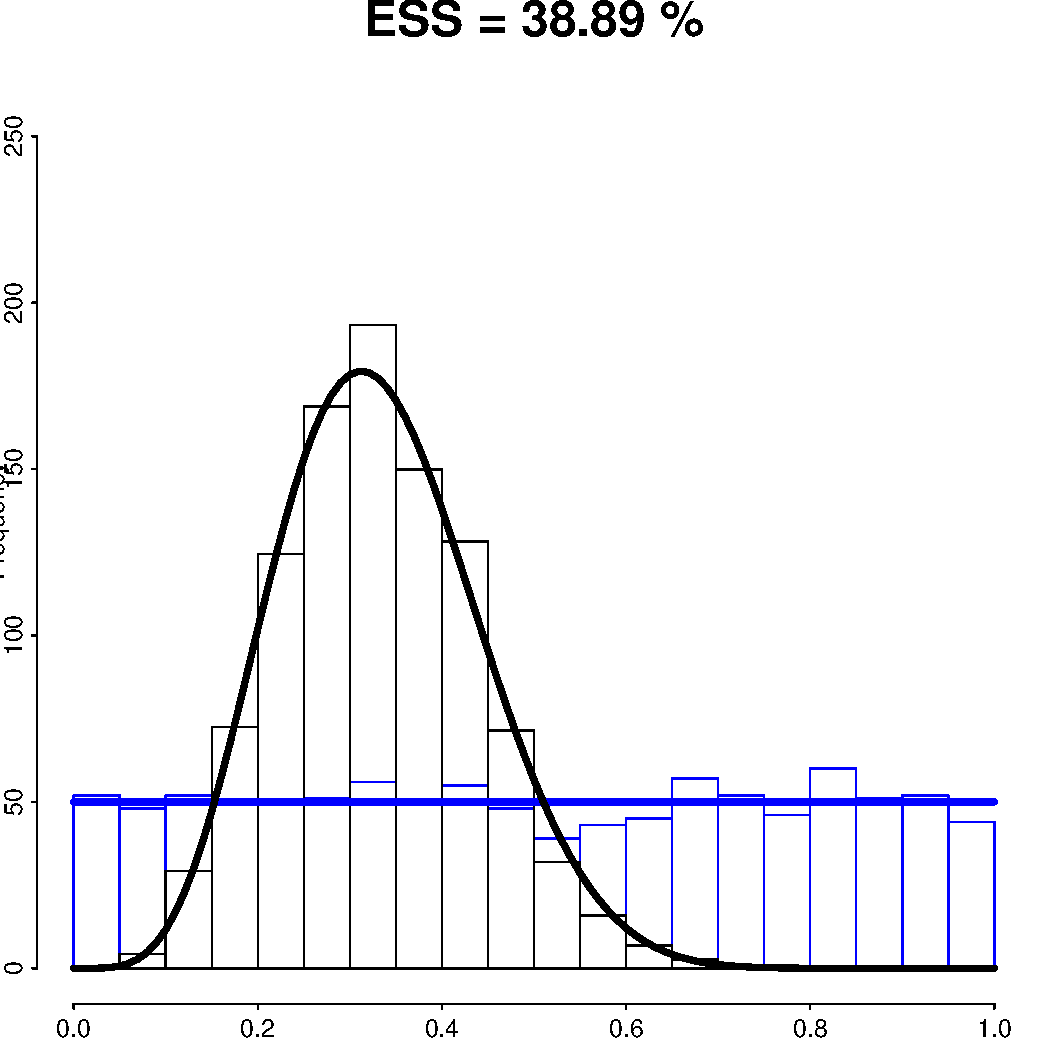
\includegraphics[height=.4\textheight]{../figs/ImportanceSampling-Beta-a06-b012-a1-b1-seed3} 
    \end{tabular}
    & 
    \begin{tabular}{c}
    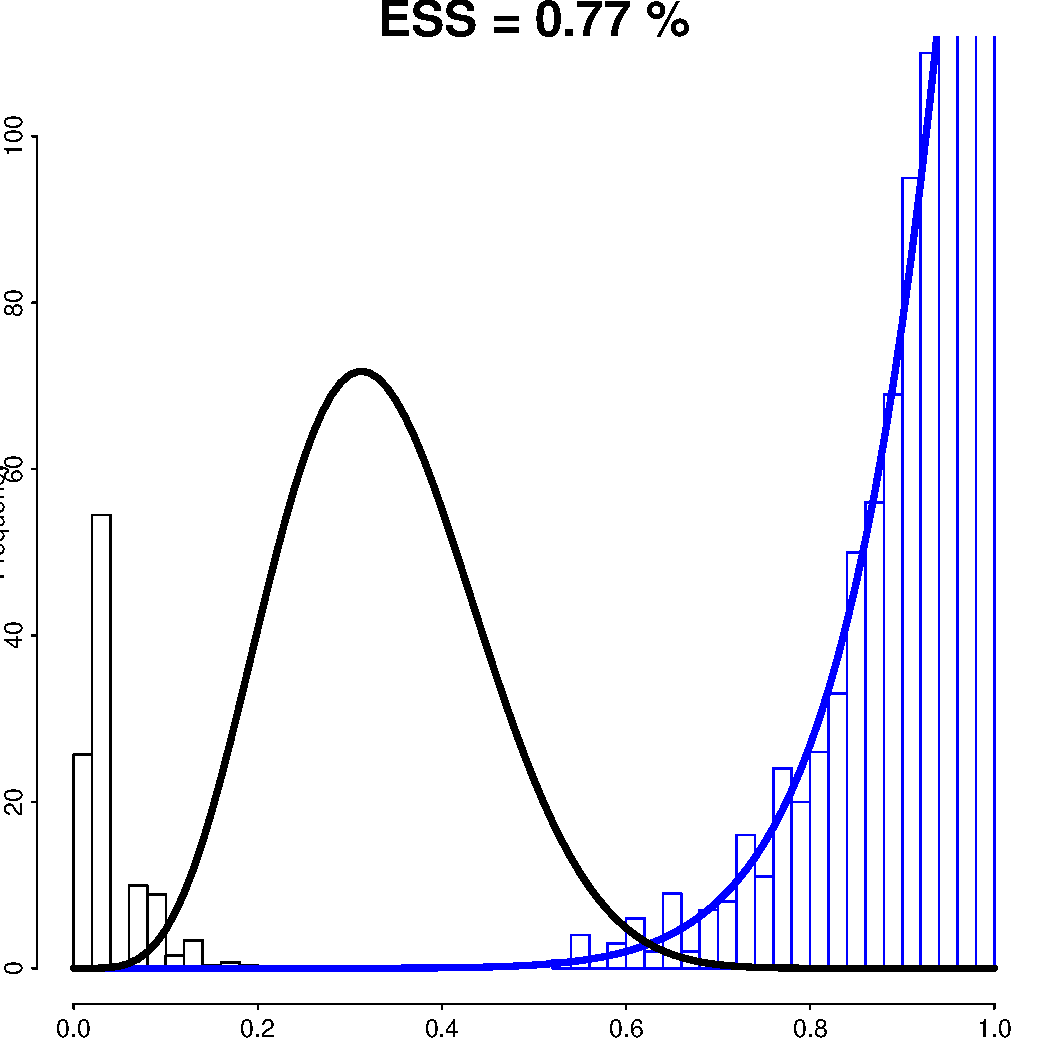
\includegraphics[height=.4\textheight]{../figs/ImportanceSampling-Beta-a06-b012-a10-b1-seed3} 
    \end{tabular}
    \\ \\
    \begin{tabular}{c}
    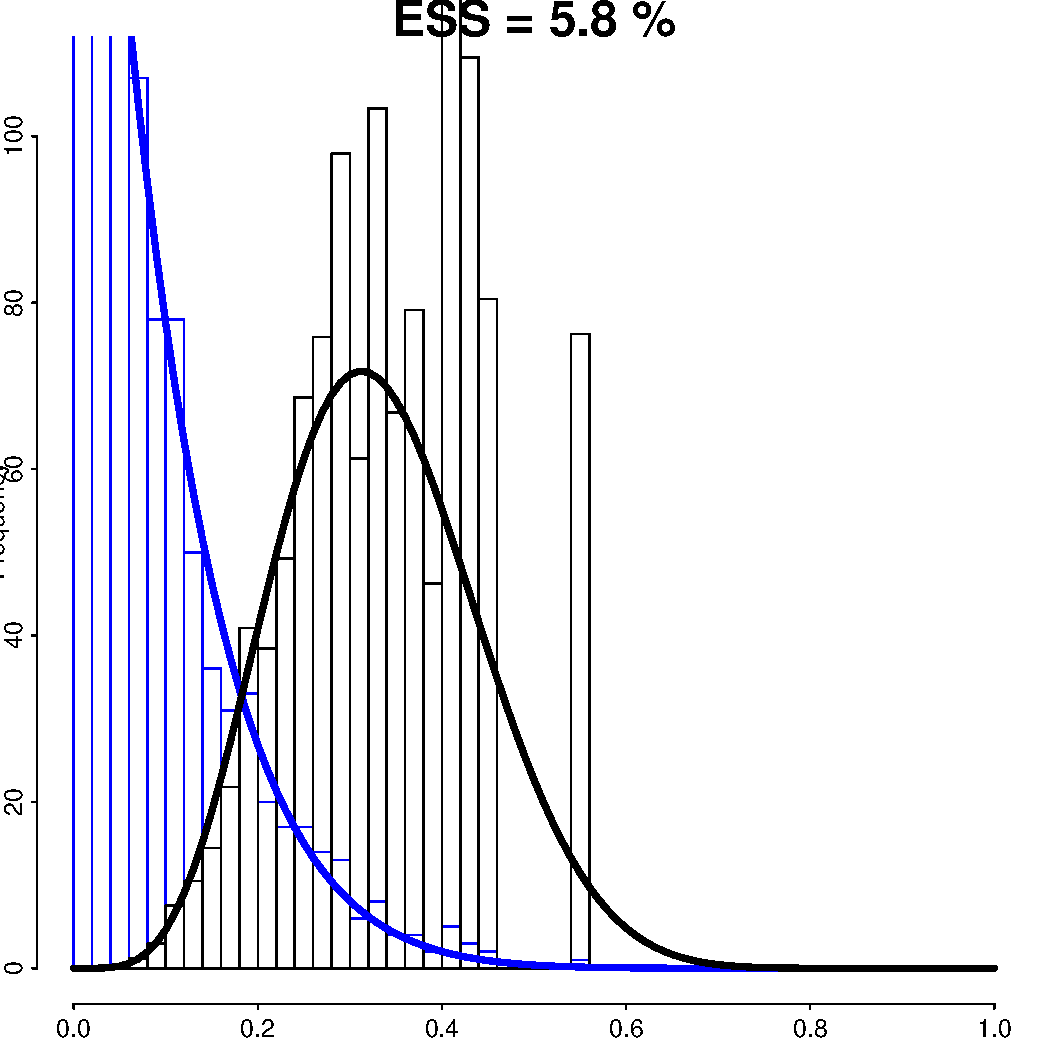
\includegraphics[height=.4\textheight]{../figs/ImportanceSampling-Beta-a06-b012-a1-b10-seed3} 
    \end{tabular}
    & 
    \begin{tabular}{c}
    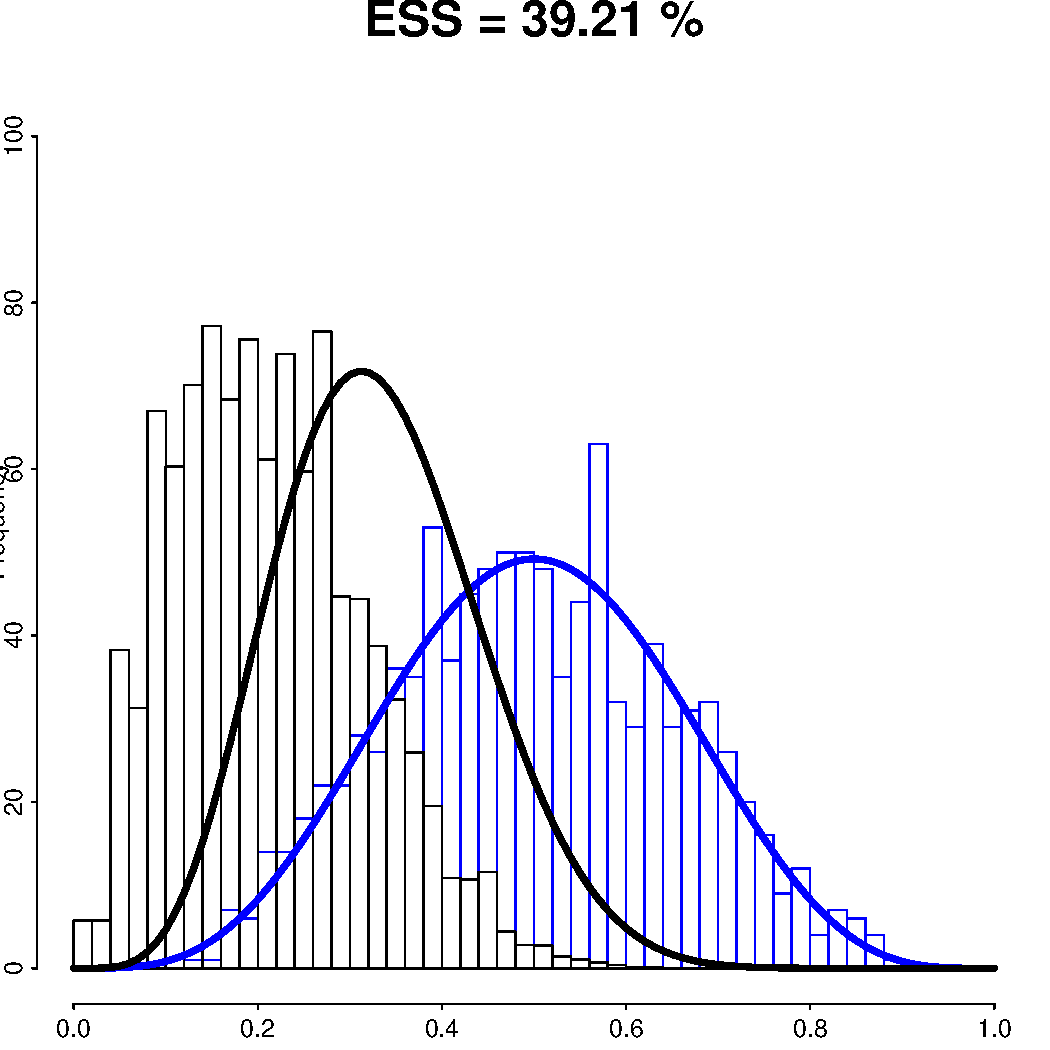
\includegraphics[height=.4\textheight]{../figs/ImportanceSampling-Beta-a06-b012-a5-b5-seed3} 
    \end{tabular}
  \end{tabular}
  \end{center}
 }  

%===================================================================
\frame{ \frametitle{Importance of the proposal: another draw}

  \begin{center}
  \begin{tabular}{cc}
    \begin{tabular}{c}
    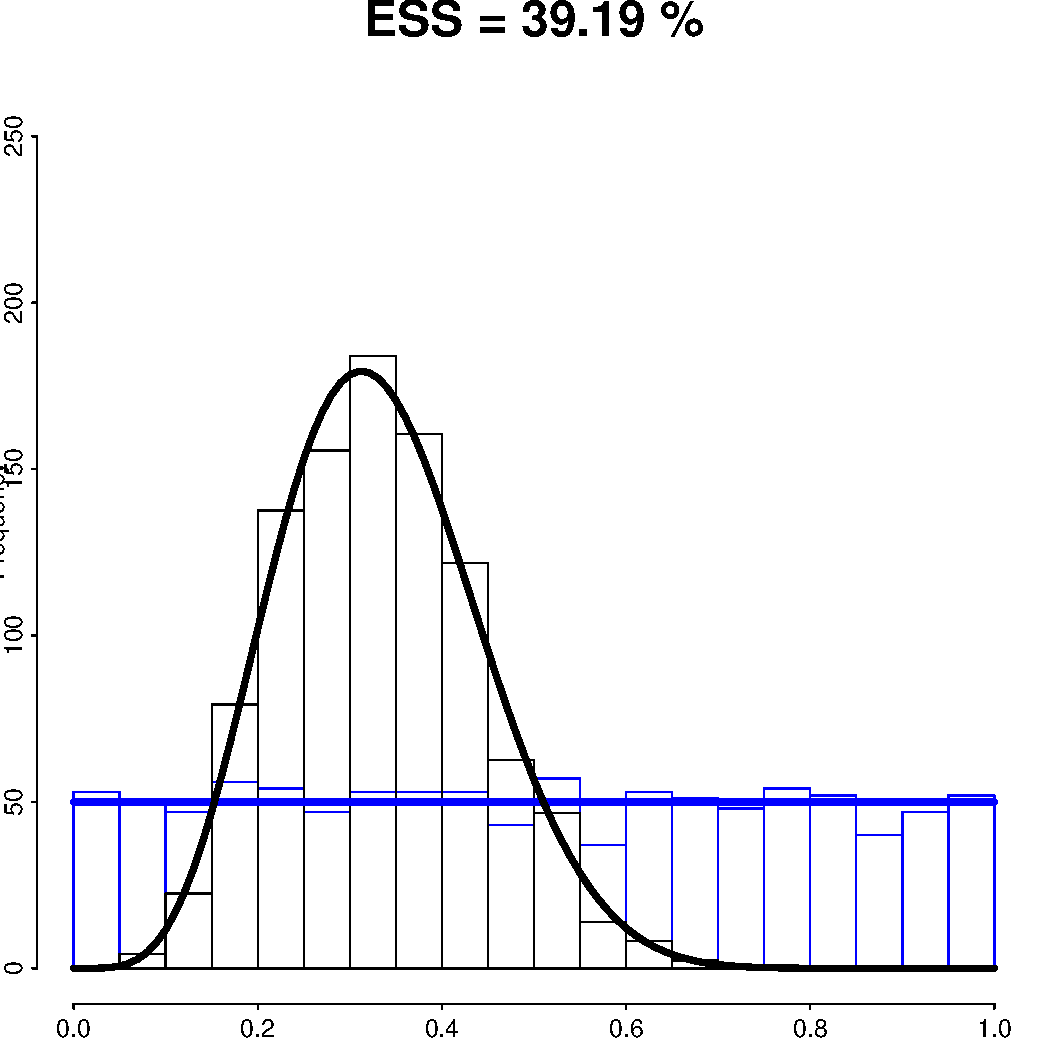
\includegraphics[height=.4\textheight]{../figs/ImportanceSampling-Beta-a06-b012-a1-b1-seed5} 
    \end{tabular}
    & 
    \begin{tabular}{c}
    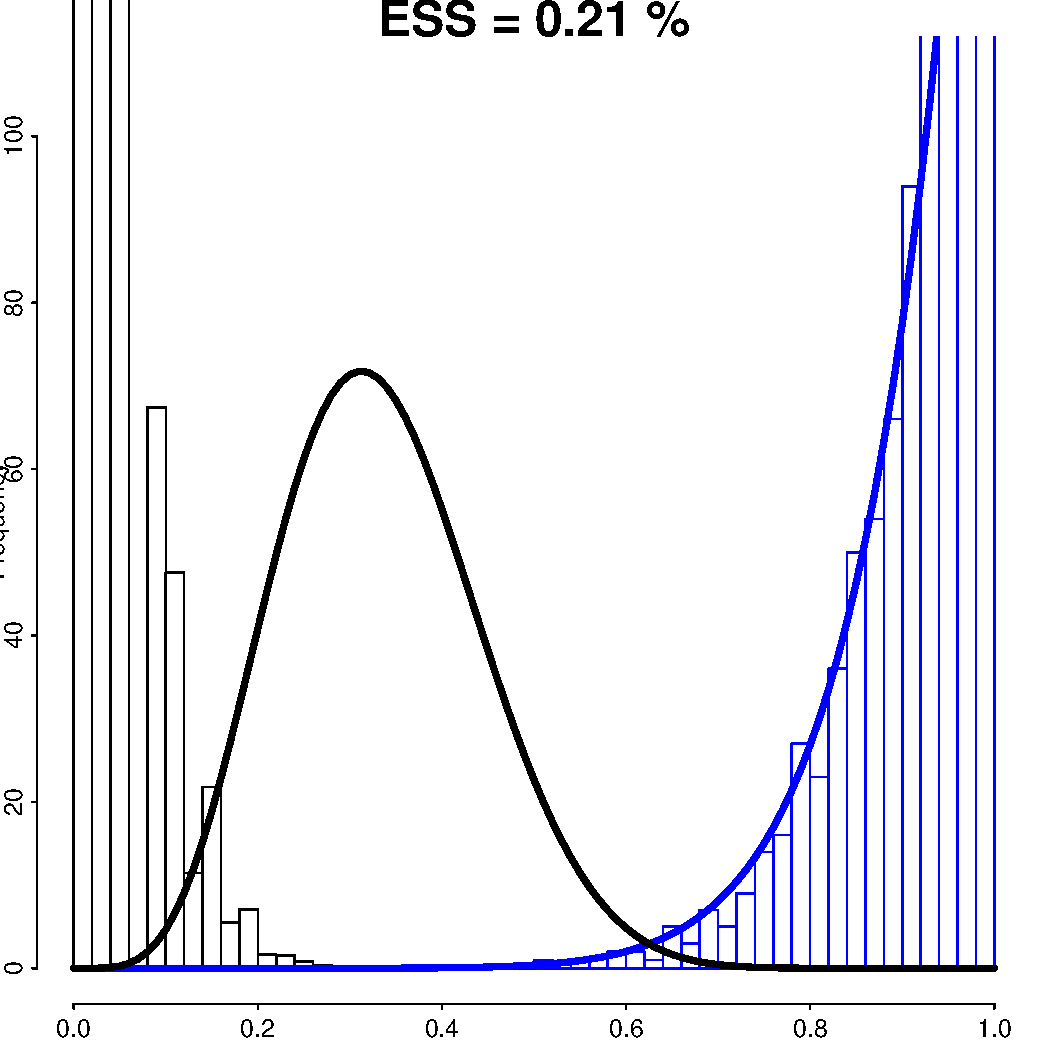
\includegraphics[height=.4\textheight]{../figs/ImportanceSampling-Beta-a06-b012-a10-b1-seed5} 
    \end{tabular}
    \\ \\
    \begin{tabular}{c}
    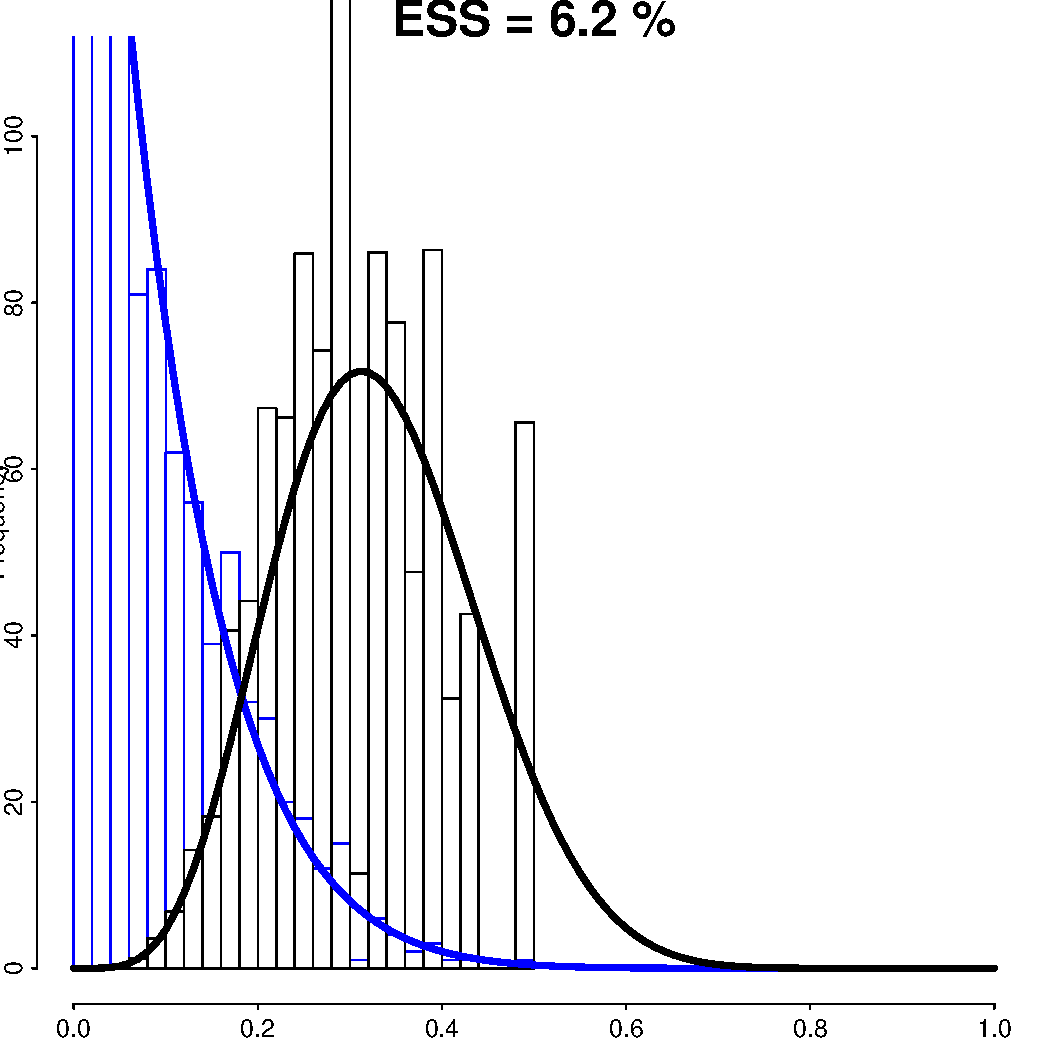
\includegraphics[height=.4\textheight]{../figs/ImportanceSampling-Beta-a06-b012-a1-b10-seed5} 
    \end{tabular}
    & 
    \begin{tabular}{c}
    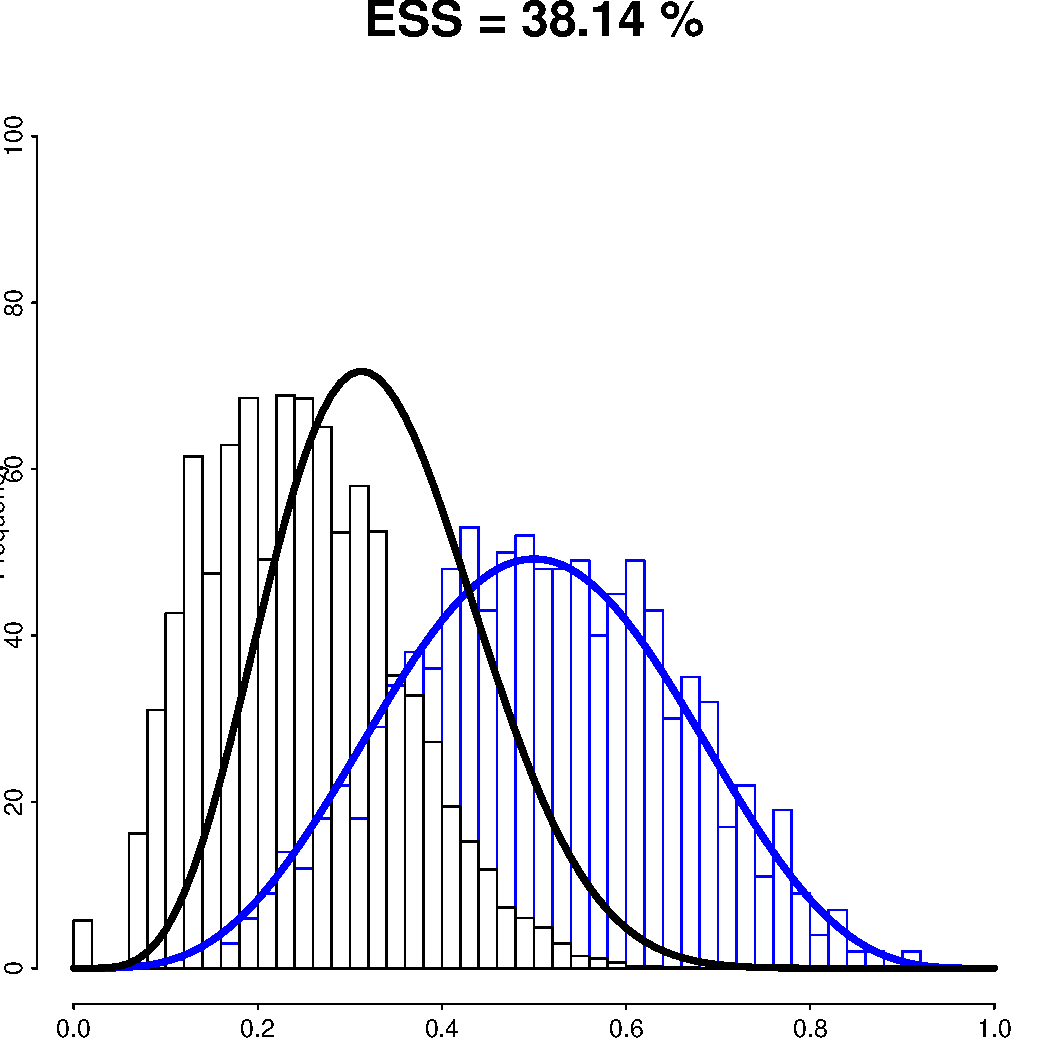
\includegraphics[height=.4\textheight]{../figs/ImportanceSampling-Beta-a06-b012-a5-b5-seed5} 
    \end{tabular}
  \end{tabular}
  \end{center}
 }  

% %===================================================================
% \frame{ \frametitle{Importance of the proposal: another draw}
% 
%   \begin{center}
%   \begin{tabular}{cc}
%     \begin{tabular}{c}
%     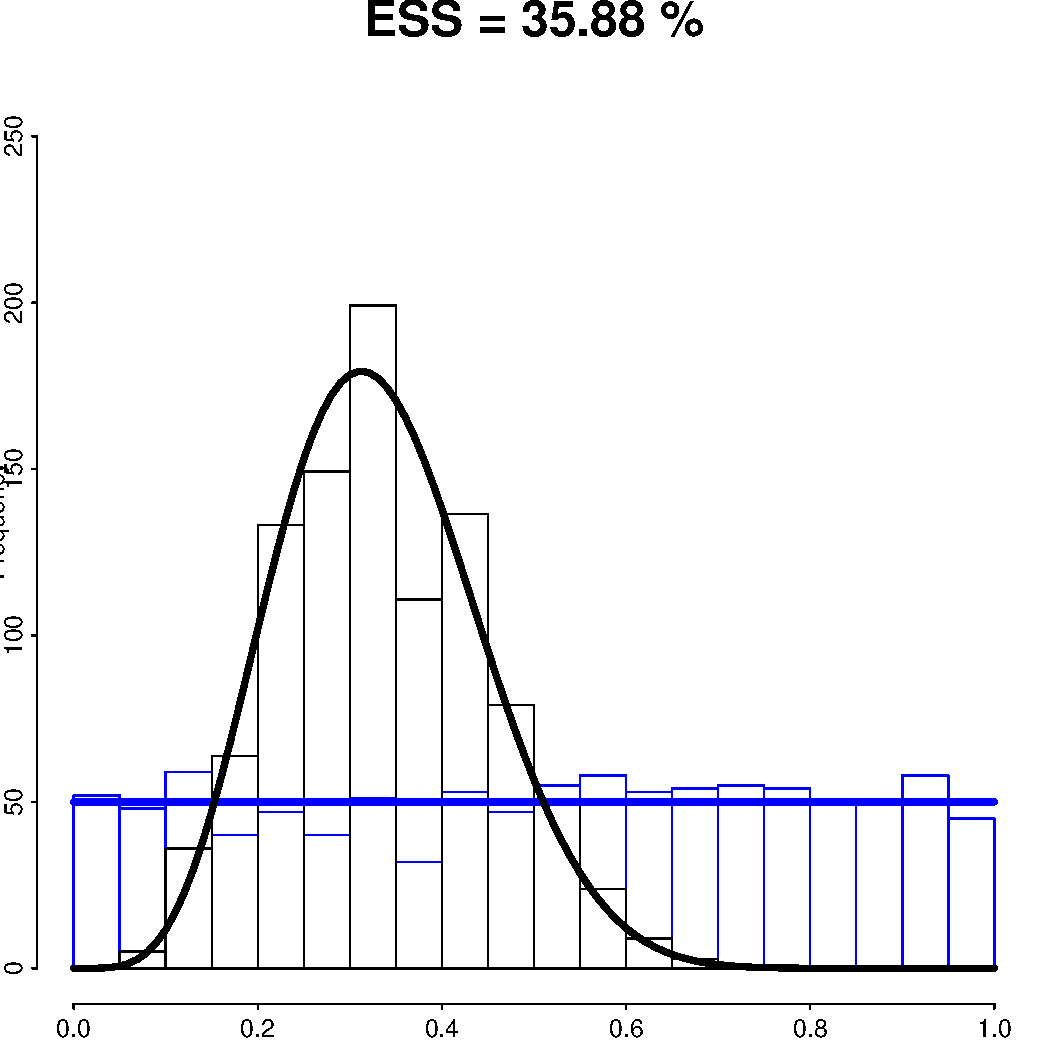
\includegraphics[height=.4\textheight]{../figs/ImportanceSampling-Beta-a06-b012-a1-b1-seed6} 
%     \end{tabular}
%     & 
%     \begin{tabular}{c}
%     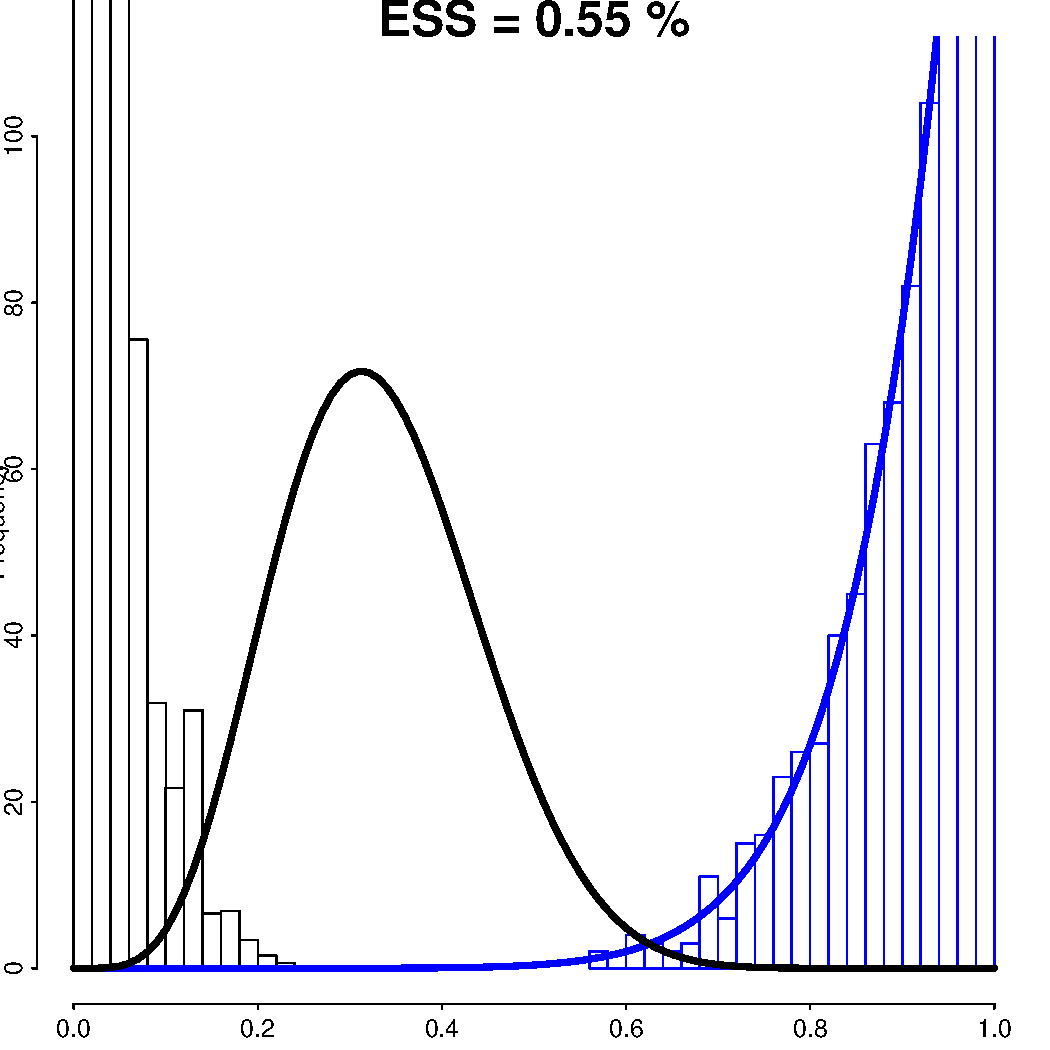
\includegraphics[height=.4\textheight]{../figs/ImportanceSampling-Beta-a06-b012-a10-b1-seed6} 
%     \end{tabular}
%     \\ \\
%     \begin{tabular}{c}
%     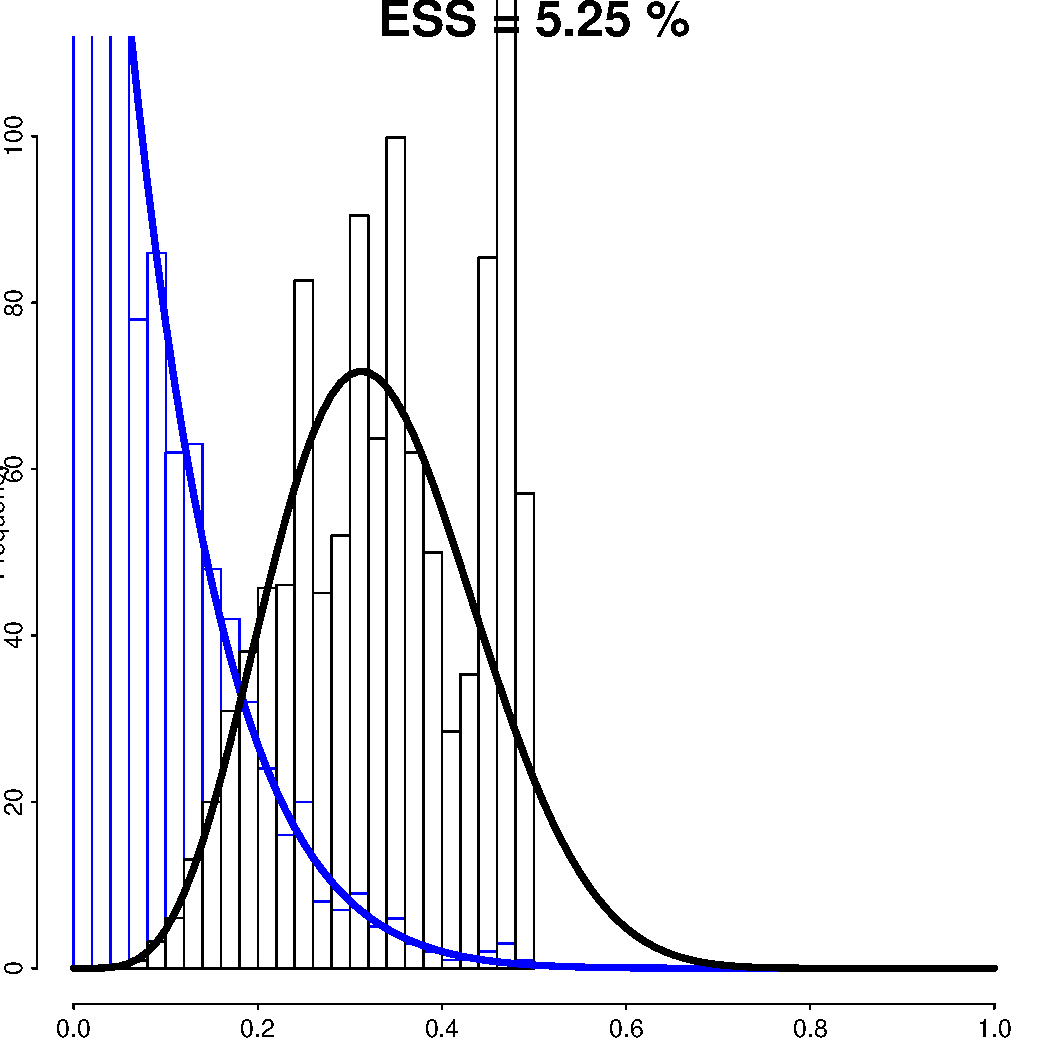
\includegraphics[height=.4\textheight]{../figs/ImportanceSampling-Beta-a06-b012-a1-b10-seed6} 
%     \end{tabular}
%     & 
%     \begin{tabular}{c}
%     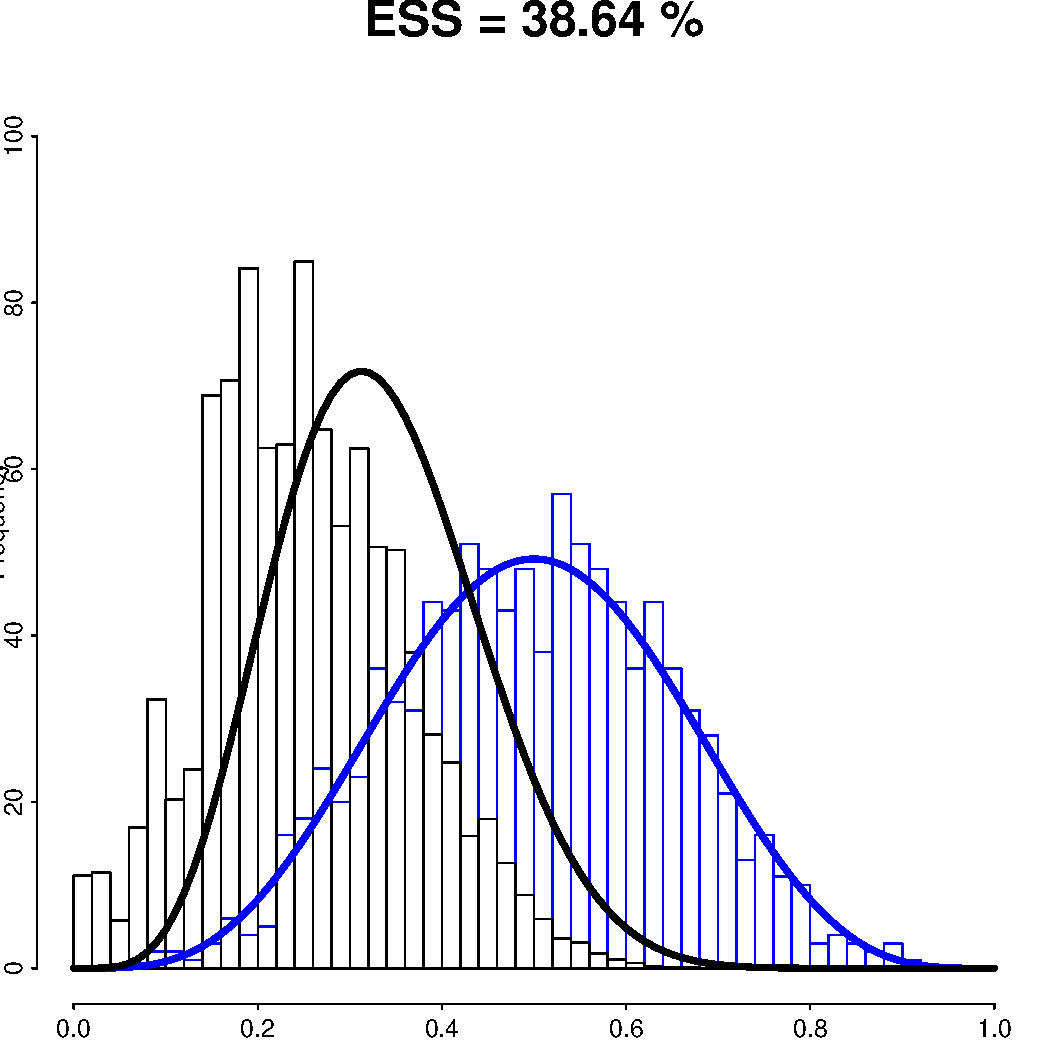
\includegraphics[height=.4\textheight]{../figs/ImportanceSampling-Beta-a06-b012-a5-b5-seed6} 
%     \end{tabular}
%   \end{tabular}
%   \end{center}
%  }  
% 
%===================================================================
\frame{ \frametitle{IS for posterior sampling}

  To evaluate $\Esp[f(\thetabf) | \Ybf]$, write it as
  \begin{align*}
    \Esp[f(\thetabf) \gv \Ybf] 
    = & \left. \int f(\thetabf) p(\thetabf, \Ybf) \d \thetabf \right/ p(\Ybf) 
    \; = \; \dots \\
%     = & \left. \int f(\thetabf) \pi(\thetabf) \ell(\Ybf \gv \thetabf) \d \thetabf \right/ \int \pi(\thetabf) \ell(\Ybf \gv \thetabf)  \d \thetabf \\
    = & \left. \int f(\thetabf) \frac{\pi(\thetabf) p(\thetabf \gv \Ybf)}{q(\thetabf)} q(\thetabf) \d \thetabf \right/ \int \frac{\pi(\thetabf) p(\thetabf \gv \Ybf)}{q(\thetabf)} q(\thetabf) \d \thetabf
  \end{align*}
  \begin{enumerate}
   \item sample
   $$
   (\thetabf^1, \dots, \thetabf^B) \text{ iid } \sim q
   $$
   \item compute the weights
   $$
   W(\thetabf^b) = \pi(\thetabf^b) p(\thetabf^b \gv \Ybf) \left/ q(\thetabf^b) \right.
   $$
   \item get
   $$
   \widehat{\Esp}[f(\thetabf) \gv \Ybf] = \sum_b W(\thetabf^b) f(\thetabf^b) \left/ \sum_b W(\thetabf^b)  \right.
   $$
   (slightly \emphase{biased}).
  \end{enumerate}
}

%===================================================================
\frame{ \frametitle{Good proposals}

  Choosing $q$ is critical

  \bigskip \pause
  \paragraph{Typical choices}
  \begin{itemize}
   \item Prior
   $$q(\thetabf) = \pi(\thetabf)$$
   \ra {far from the target $p(\thetabf \gv \Ybf)$: small $ESS$} \\ ~
   \item \pause MLE: 
   $$q(\thetabf) = \Ncal(\widehat{\thetabf}_{MLE}, \Var_\infty(\widehat{\thetabf}_{MLE}))$$  
   \ra {fine, as long as MLE is available} \\ ~
   \item \pause Variational Bayes, expectation propagation, ...: 
   $$
   q(\thetabf) = \arg\min_{q \in \Qcal} KL\left[q(\thetabf) \,||\, p(\thetabf \gv \Ybf\right]
   $$
   \ra fast and reasonably accurate
  \end{itemize}
}

%===================================================================
\frame{ \frametitle{Variational Bayes \& ML as a prior}

  $\textcolor{blue}{\boldsymbol{-}}:$ prior, $\textcolor{red}{\boldsymbol{-}}:$ VB, $\textcolor{green}{\boldsymbol{-}}:$ MLE, $\boldsymbol{-}:$ posterior 
  $$
  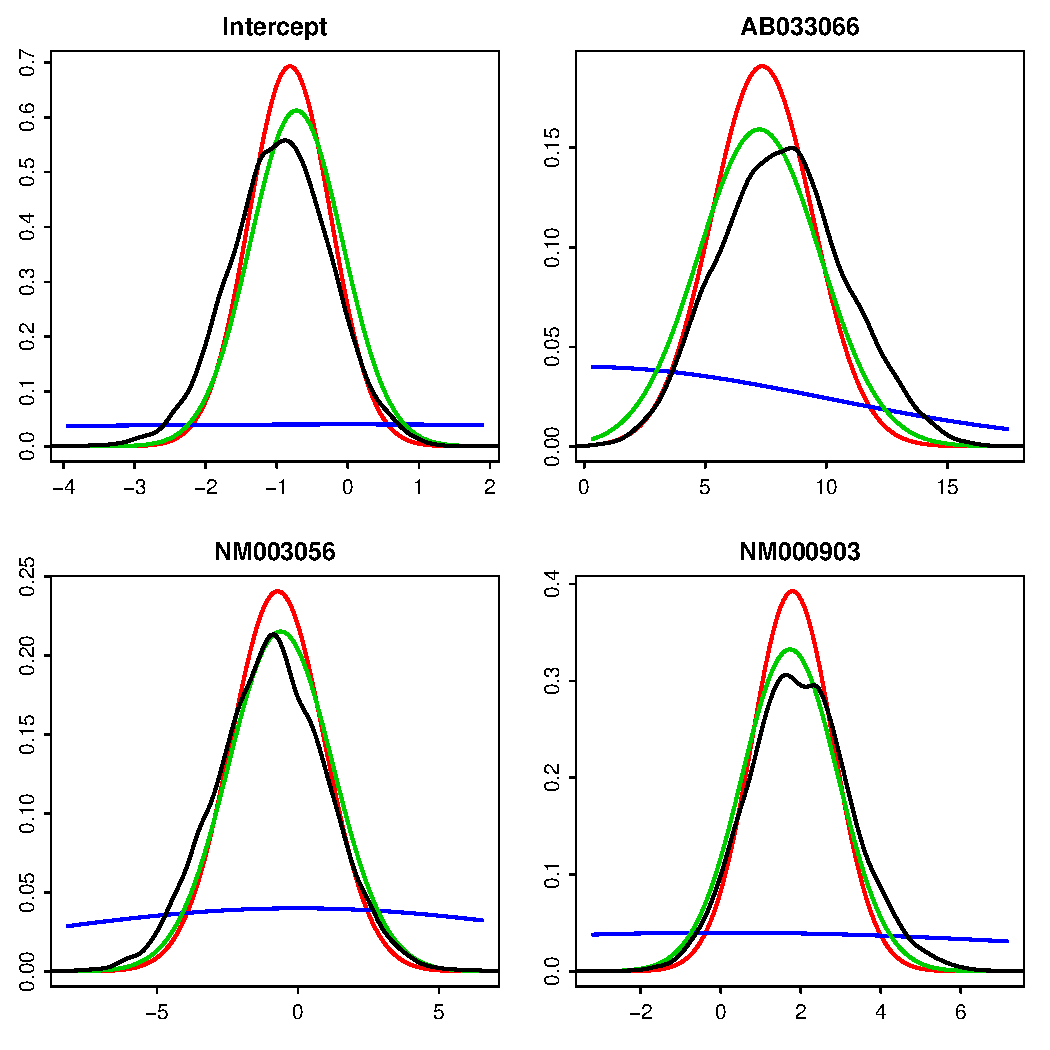
\includegraphics[width=.8\textwidth, height=.8\textheight]{\figfig/ISproposal-density}
  $$
}

%===================================================================
\frame{ \frametitle{Variational Bayes as a prior: joint distribution}

  $\textcolor{red}{\boldsymbol{-}}:$ VB, $\boldsymbol{-}:$ posterior 
  $$
  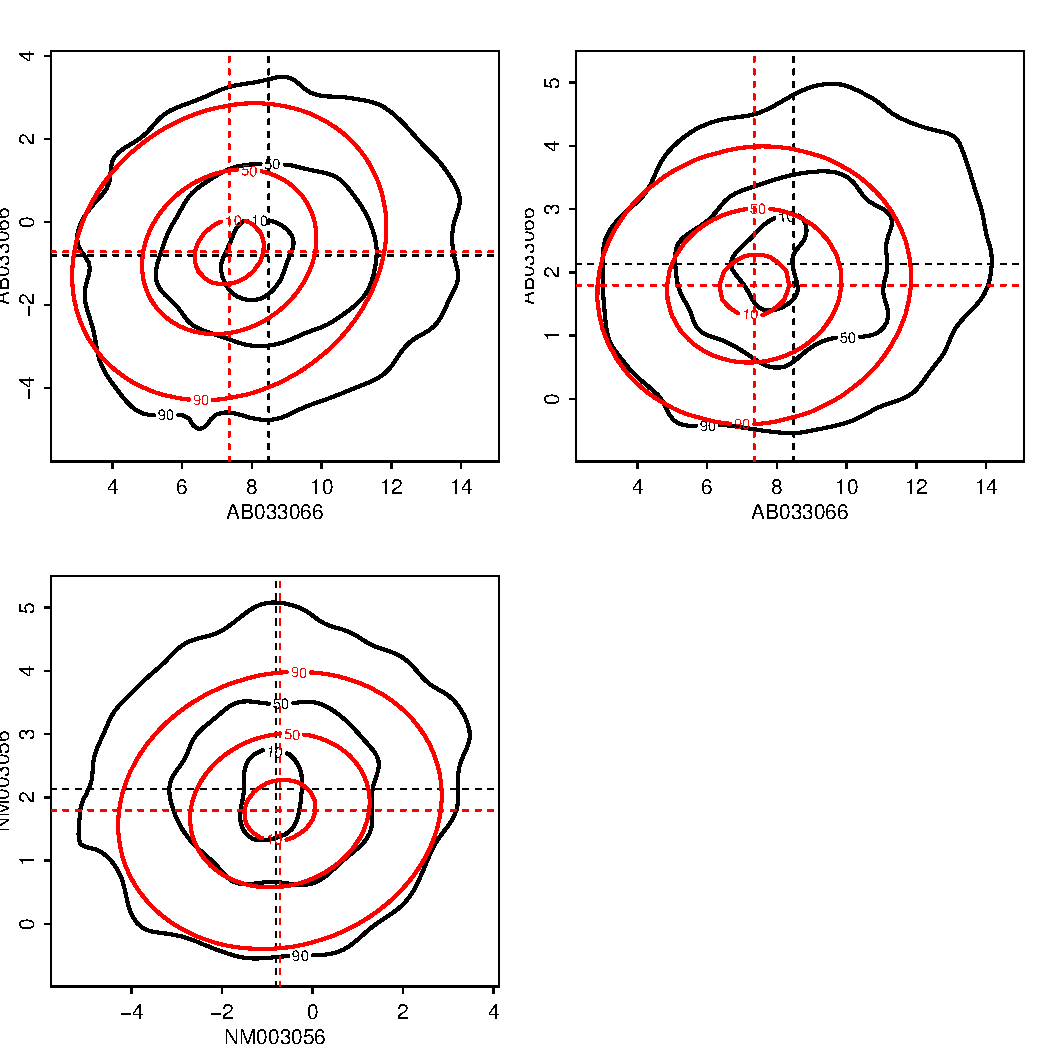
\includegraphics[width=.8\textwidth, height=.8\textheight]{\figfig/ISproposal-density2D}
  $$
}

%====================================================================
\subsection{Monte Carlo Markov chains (MCMC)}
\frame{\frametitle{Outline} \tableofcontents[currentsubsection]}
%====================================================================
\frame{ \frametitle{Limit distribution of Markov chain}

  \paragraph{Property.} If $\{\phibf^b\}_{b \geq 0}$ is an ergodic Markov chain (irreducible, aperiodic, ...) with
  \begin{itemize}
   \item initial distribution $\phibf^0 \sim \nu$,
   \item transition kernel $\phibf^b \gv \phibf^{b-1} \sim \kappa(\cdot \gv \phibf^{b-1})$:
  \end{itemize}
  $$
  p\left(\{\phibf^b\} \right) = \nu(\phibf^0) \times \kappa(\phibf^1 \gv \phibf^0) \times \kappa(\phibf^2 \gv \phibf^1) \times \kappa(\phibf^3 \gv \phibf^2) \times \dots
%   \prod_{b\geq 1} \kappa(\phibf^b \gv \phibf^{b-1})
  $$
  then
  \begin{itemize}
   \item it admits a \emphase{unique stationary distribution} $\mu$:
   $$
   \phibf^{b-1} \sim \mu \qquad \Rightarrow \qquad \phibf^b \sim \mu
   $$
   \item $\phibf^b$ converges towards $\mu$ in distribution
   $$
   \phibf^b \overset{\Delta}{\underset{b \rightarrow \infty}{\longrightarrow}} \mu
   $$
   for \emphase{any initial distribution} $\nu$
  \end{itemize}
}

%====================================================================
\frame{ \frametitle{Use for Bayesian inference}

  \paragraph{Aim.} Sample from
  $$
  p(\thetabf \gv \Ybf)
  $$
  
  \paragraph{Idea.} 
  \begin{itemize}
   \item Construct an ergodic Markov chain $\{\thetabf^b\}_{b \geq 0}$ with stationary distribution
   $$
   \mu(\thetabf) = p(\thetabf \gv \Ybf)
   $$
   \item Choose 'any' initial $\nu$ and simulate $\{\thetabf^b\}_{b \geq 0}$ \\ ~
   \item Until it 'reaches' its stationary distribution
  \end{itemize}
}

%====================================================================
\frame{ \frametitle{Metropolis-Hastings}

  \paragraph{Algorithm.} Define a shift kernel $\lambda(\cdot \gv \thetabf)$
  \begin{itemize}
   \item \pause Start with $\thetabf^0$
   \item \pause At step $b$, 
   \begin{enumerate}
    \item \pause sample $\thetabf' \sim \lambda(\cdot \gv \thetabf^{b-1})$;
   \item \pause compute the Metropolis-Hastings ratio (acceptance probability)
   $$
   \alpha(\thetabf', \thetabf^{b-1}) 
   = \frac{\lambda(\thetabf^{b-1} \gv \thetabf')}{\lambda(\thetabf' \gv \thetabf^{b-1})} \frac{p(\thetabf' \gv \Ybf)}{p(\thetabf^{b-1} \gv \Ybf)}
   \pause = \frac{\lambda(\thetabf^{b-1} \gv \thetabf')}{\lambda(\thetabf' \gv \thetabf^{b-1})} \frac{\pi(\thetabf') \ell(\Ybf \gv \thetabf')}{\pi(\thetabf^{b-1}) \ell(\Ybf \gv \thetabf^{b-1})};
   $$
   \item \pause $\text{set } \thetabf^b= \left\{
	 \begin{array}{ll}
	   \thetabf' & \text{with probability $\max(1, \alpha(\thetabf', \thetabf^{b-1}))$,} \\
	   \thetabf^{b-1} & \text{otherwise.}
	 \end{array} 
    \right.$
   \end{enumerate}
  \end{itemize}
  
  \bigskip \pause
  \paragraph{Properties.} 
  \begin{enumerate}
   \item $\lambda$ and $\alpha$ define a Markov chain with stationary distribution $\mu(\thetabf) = p(\thetabf \gv \Ybf)$.
   \item If $\lambda(\cdot \gv \thetabf)$ is symmetric, $\alpha$ reduce to ${\pi(\thetabf') \ell(\Ybf \gv \thetabf')}/ [{\pi(\thetabf^{b-1}) \ell(\Ybf \gv \thetabf^{b-1})}]$
  \end{enumerate}
}

%====================================================================
\frame{ \frametitle{Metropolis-Hastings for logistic regression}

  \paragraph{Model.} 
  \begin{align*}
   \thetabf & \sim \pi(\thetabf) = \Ncal(\Obf_p, 100 \, \Ibf_p)\\
   \Ybf \gv \thetabf & \sim \ell(\Ybf \gv \thetabf) 
   = \prod_i \left(\frac{e^{\xbf_i^\intercal \thetabf}}{1 + e^{\xbf_i^\intercal \thetabf}}\right)^{y_i} \left(\frac{e^{\xbf_i^\intercal \thetabf}}{1 + e^{\xbf_i^\intercal \thetabf}}\right)^{1-y_i}
  \end{align*}

  \bigskip \bigskip \pause
  \paragraph{Algorithm settings.} 
  $$\thetabf^0 = \Obf_p$$
  $$\lambda( \cdot \gv \thetabf) = \Ncal(\Obf_p, .5 \, \Ibf_p)$$
}

%====================================================================
\frame{ \frametitle{M-H for logistic regression: R code}

  \pause
  \footnotesize{\tt 
  mu.prior = rep(0, p); Sigma.prior = 100*diag(p); Sigma.shift = .5*diag(p) \\ \pause
  theta.sample = matrix(0, B, p); \\ \pause
  ~ \\
  theta.cur = theta.sample[1, ] \\ \pause
  logprior.cur = dmvnorm(theta.cur, mean=mu.prior, sigma=Sigma.prior, log=T) \\ \pause
  prob.cur = plogis(X\%*\%theta.cur) \\ \pause
  loglik.cur = sum(dbinom(Y, 1, prob.cur, log=T)) \\ \pause
  ~ \\
  for (b in 2:B)\{ \\ \pause
  \qquad theta.prop = rmvnorm(1, mean=theta.sample[b-1, ], sigma=Sigma.shift)[1, ] \\ \pause
  \qquad logprior.prop = dmvnorm(theta.prop, mean=mu.prior, sigma=Sigma.prior, log=T) \\ \pause
  \qquad prob.prop = plogis(X\%*\%theta.prop) \\ \pause
  \qquad loglik.prop = sum(dbinom(Y, 1, prob.prop, log=T)) \\ \pause
  ~ \\
  \qquad alpha = exp(logprior.prop + loglik.prop - logprior.cur - loglik.cur) \\ \pause
  \qquad if(runif(1) < alpha)\{ \\ 
  \qquad \qquad theta.sample[b, ] = theta.cur = theta.prop \\ 
  \qquad \qquad logprior.cur = logprior.prop; loglik.cur = loglik.prop \\ \pause
  \qquad \}else\{ \\
  \qquad \qquad theta.sample[b, ] = theta.sample[b-1, ] \\
  \qquad \} \\ \pause
  \} \\
  }
}

%====================================================================
\frame{ \frametitle{Sanity checks}

  \bigskip
  \paragraph{Setting.} Sample $1.2 \; 10^5$ $\thetabf$, remove first $2 \; 10^4$, extract every 10 \ra $B = 10^4$. \\ ~

  \begin{tabular}{cc}
    \begin{tabular}{p{.3\textwidth}}
	 \begin{itemize}
	 \item \onslide+<1->{Acceptance rate} \\ ~
	 \item \onslide+<2->{Stationarity: \\ 
	   var. shift = .1} 
	   \onslide+<3->{, .5} 
	   \onslide+<4->{, 1 \\ ~}
	 \item \onslide+<5->{Autocorrelation  
	   $\Cor(\theta_j^{b-1}, \theta_j^b)$: \\
	   var. shift = .1} 
	   \onslide+<6->{, .5} 
	   \onslide+<7->{, 1 \\ ~}
	 \item \onslide+<8->{And many others (e.g. Gelman-Rubin)}
	 \end{itemize}
	 \\~ \\~ \\~ \\~ \\~ \\~ \\~ \\~ 
    \end{tabular}
    & 
    \hspace{-.02\textwidth}
    \begin{tabular}{p{.7\textwidth}}
	 \begin{overprint}
	 %===================
	  \onslide<1>
	  \vspace{.3\textheight}
	  \begin{tabular}{lrrrr}
	   variance shift & 0.1  & 0.5  & 1 \\ 
	   \hline 
	   acceptance rate  & 0.421  & 0.125  & 0.053 
	   \end{tabular} 
	 %=================
	  \onslide<2>
	  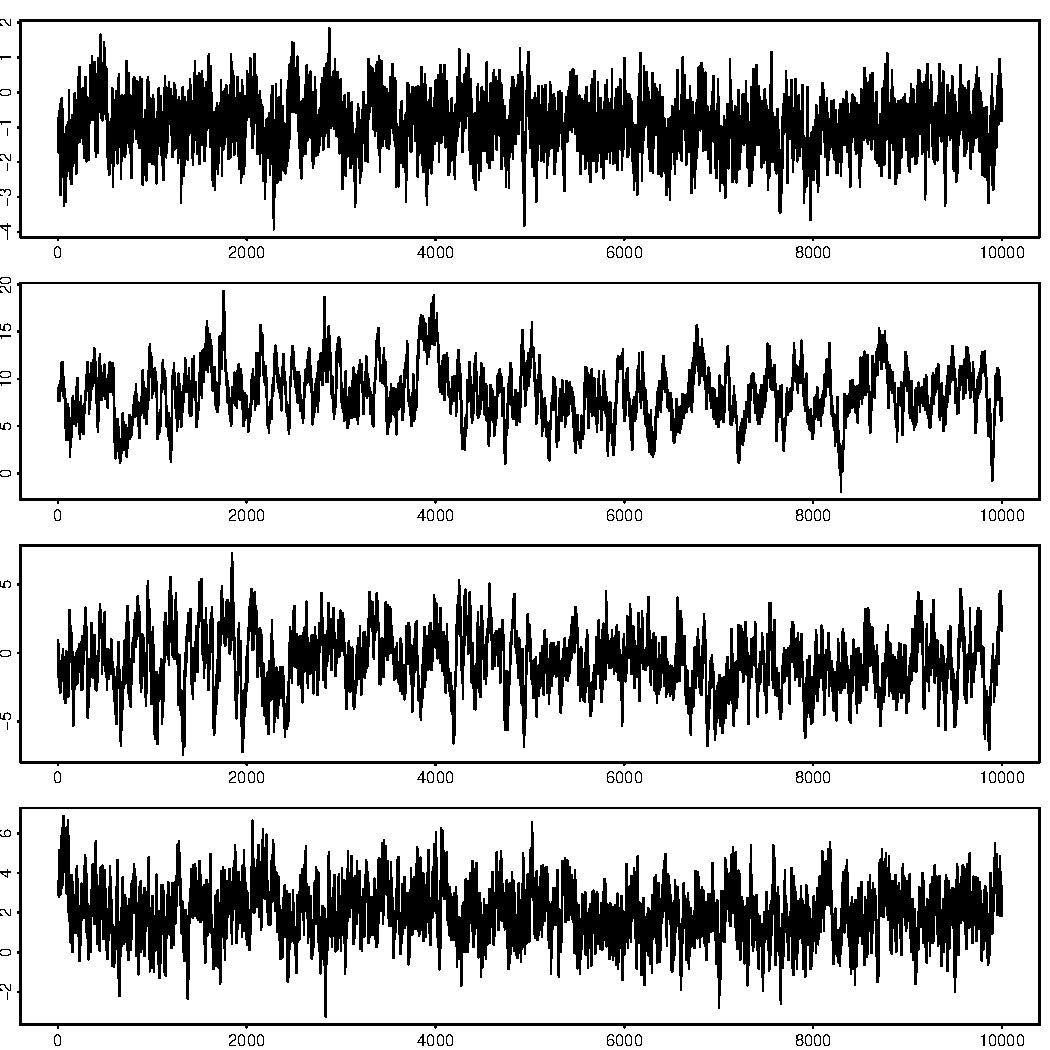
\includegraphics[width=.5\textwidth]{../figs/MH-path-10shift1}
	 %=================
	  \onslide<3>
	  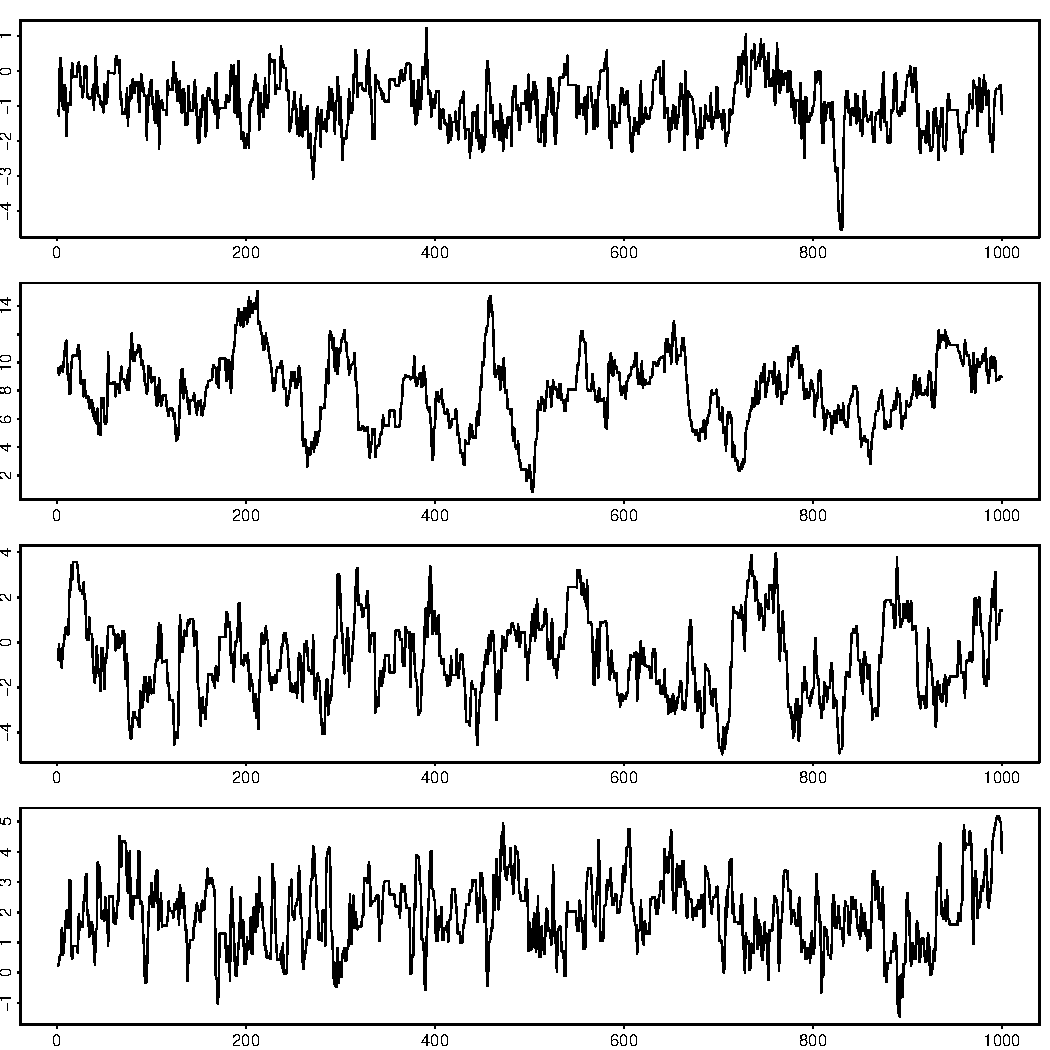
\includegraphics[width=.5\textwidth]{../figs/MH-path-10shift5}
	 %=================
	  \onslide<4>
	  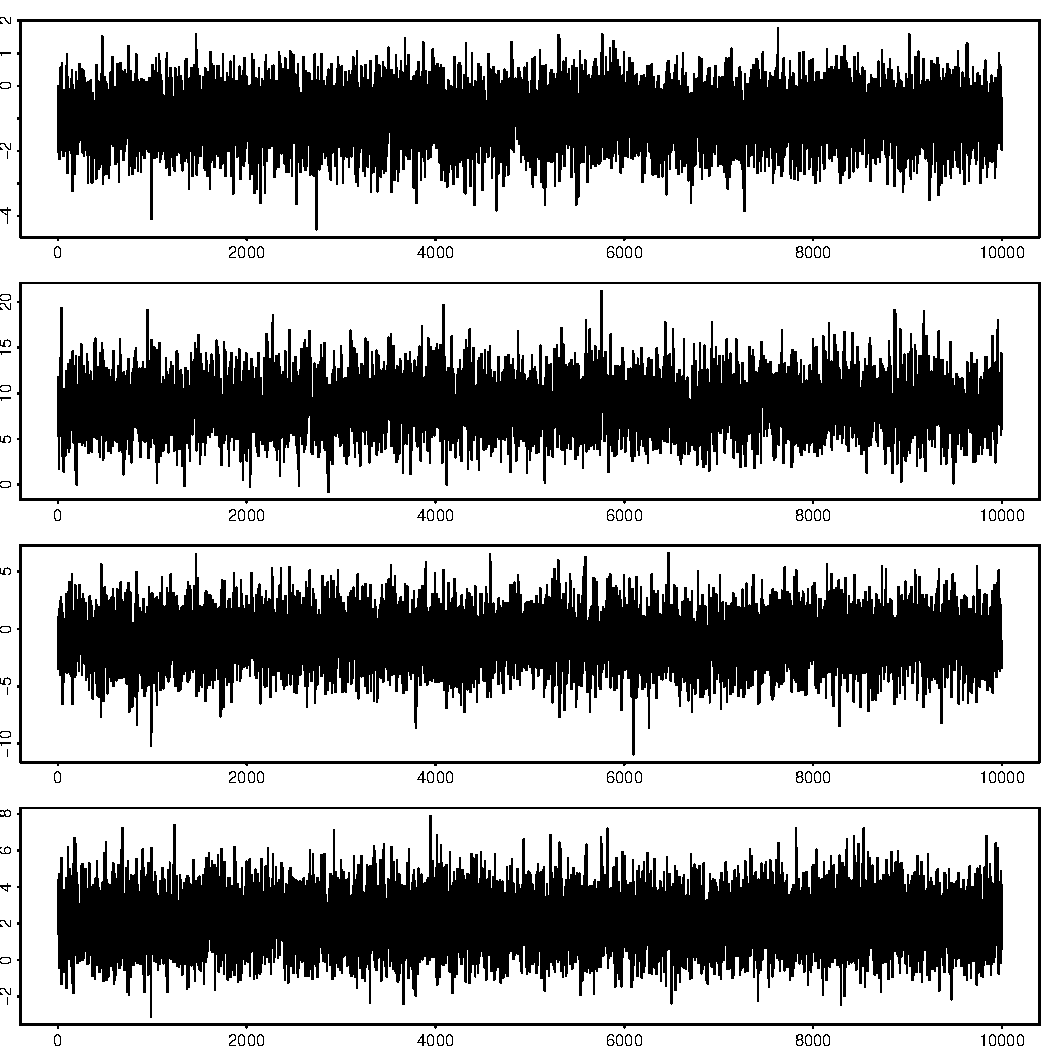
\includegraphics[width=.5\textwidth]{../figs/MH-path-10shift10}
	 %=================
	  \onslide<5>
	  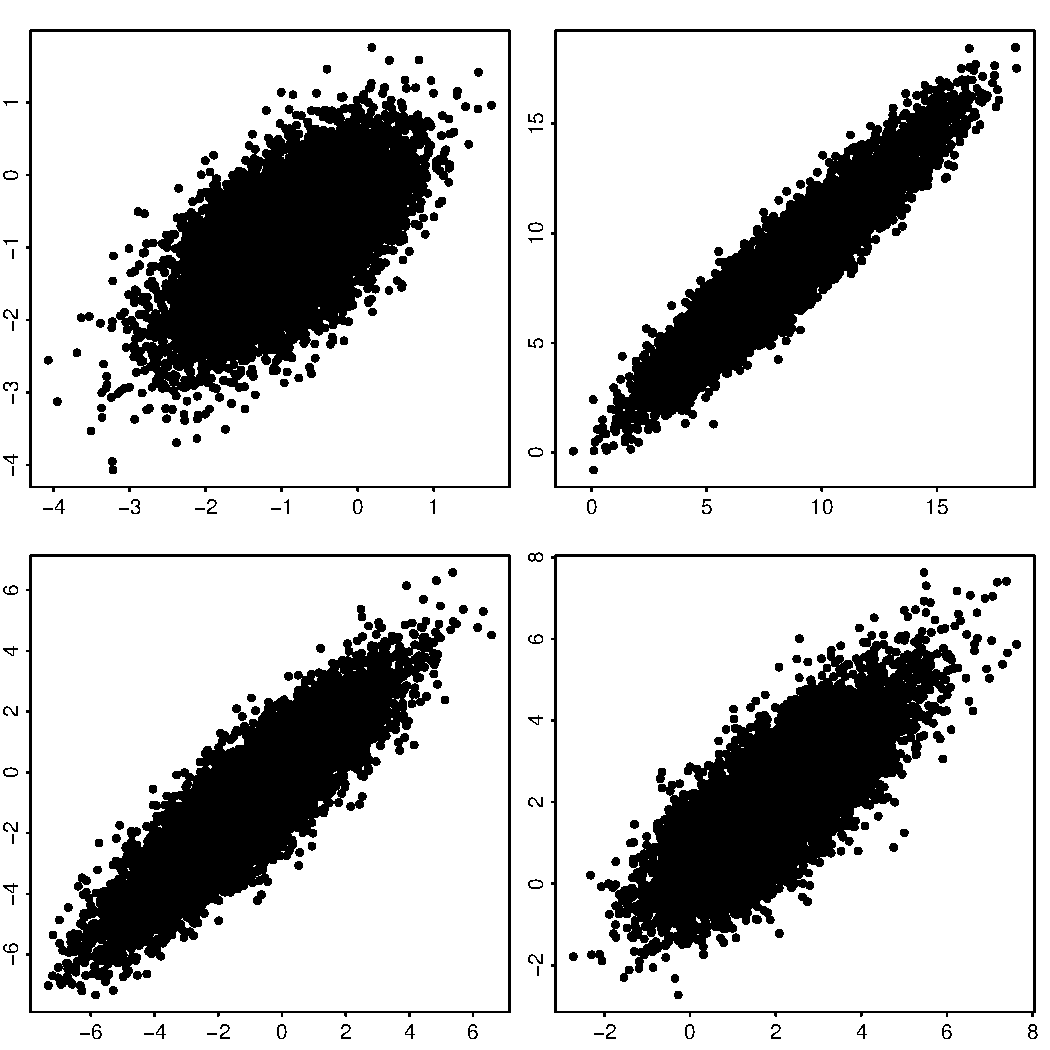
\includegraphics[width=.5\textwidth]{../figs/MH-autocorrelation-10shift1}
	 %=================
	  \onslide<6>
	  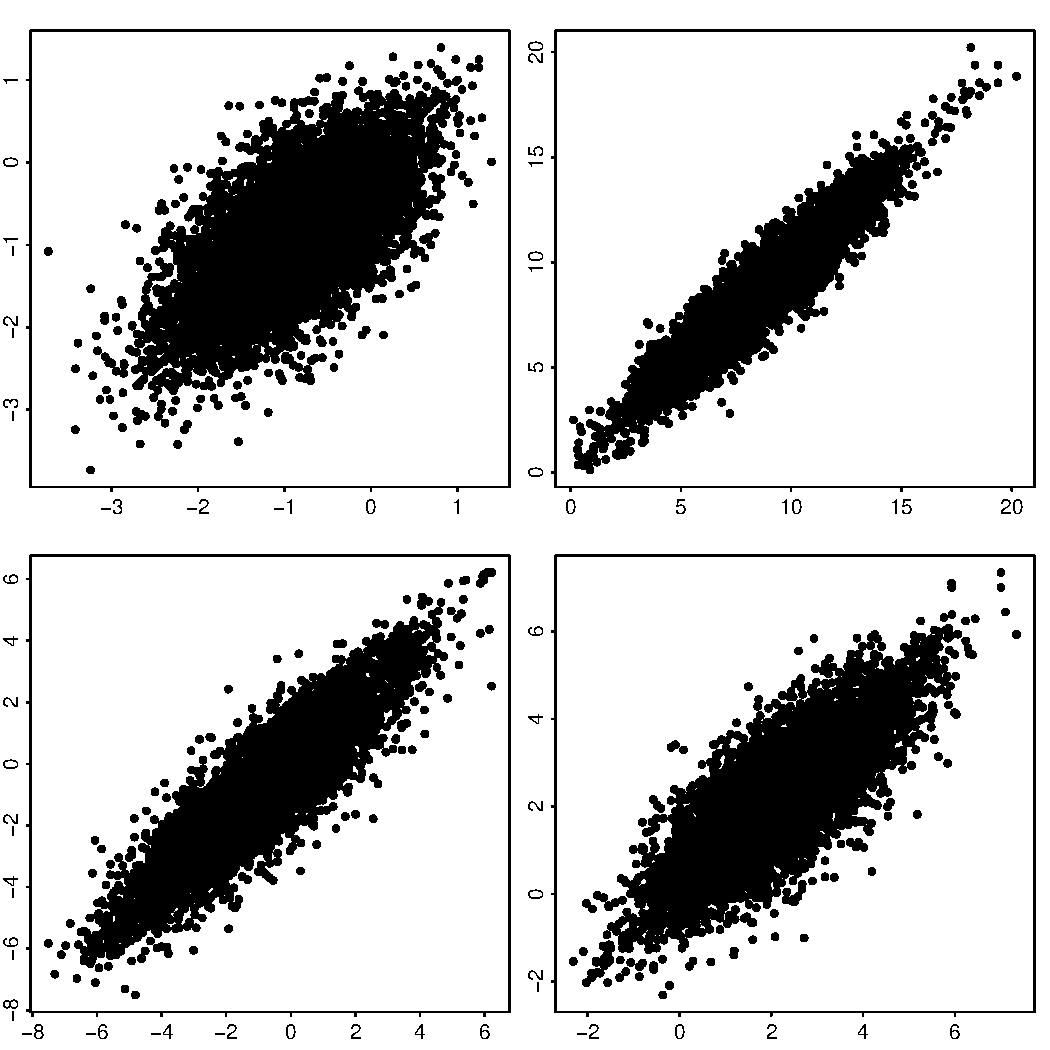
\includegraphics[width=.5\textwidth]{../figs/MH-autocorrelation-10shift5}
	 %=================
	  \onslide<7->
	  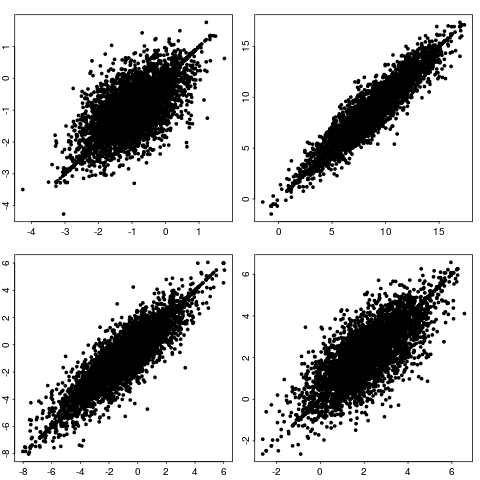
\includegraphics[width=.5\textwidth]{../figs/MH-autocorrelation-10shift10}
	 \end{overprint}
    \end{tabular}
  \end{tabular}
}

%====================================================================
\frame{ \frametitle{Gibbs}

  \paragraph{Framework.} We do not know how to sample the whole vector $\thetabf$:
  $$
  p(\thetabf \gv \Ybf)
  $$
  but we may know how to sample each coordinate (conditional on the others):
  $$
  p(\theta_j \gv \Ybf, \thetabf_{-j})
  $$
  $\thetabf_{-j} = (\theta_1, \dots, \theta_{j-1}, \theta_{j+1}, \dots \theta_p)$.
  
  \pause \bigskip \bigskip
  \paragraph{Sampling a genotype.}
  \begin{itemize}
   \item Hard to sample a whole genotype (accounting for linkage disequilibrium)
   \item Easy to sample the genotype at one locus, conditional on the rest of the genotype
  \end{itemize}
}

%====================================================================
\frame{ \frametitle{Gibbs sampling for Bayesian inference}

  \paragraph{Algorithm.} Sample $\{\thetabf^b\}_{b=0 ,\dots B}$ as follows.
  \begin{itemize}
   \item \pause Start with $\thetabf^0$
   \item \pause At step $b$, for $j = 1, \dots p$, sample $\theta_j^b$:
   $$
   \theta_j^b \gv \Ybf, \theta_1^b, \dots, \theta_{j-1}^b, \theta_{j+1}^{b-1}, \dots, \theta_{j+1}^{b-1}
   $$
  \end{itemize}

  \pause \bigskip  \bigskip
  \paragraph{Property.}
  \begin{itemize}
   \item Obviously, $p(\thetabf \gv \Ybf)$ is a stationary distribution.
   \item Does not suffices to prove ergodicity.
  \end{itemize}
  }

% %====================================================================
% \frame{ \frametitle{Example: sampling allelic frequencies}
% 
%   \paragraph{Model.} 2 alleles / marker.
%   % Useless: conjugate prior!!!
%   \begin{itemize} 
%    \item $p$ loci, $n$ individuals, 
%    \item $Y_{ij} =$ genotype of individual $i$ at locus $j$ $\in \{0, 1\}$
%    \item $\thetabf = (\theta_y)_{y \in \{0, 1\}^p}$
%    \item Prior: $\thetabf \sim \Dcal(\dbf)$, $\dbf = (d_y)$
%   \end{itemize}
%   
%   }


%====================================================================
\section{Extensions} \label{sec:ABC}
\frame{\frametitle{Outline} \tableofcontents[currentsection]}
%====================================================================
\subsection{Sequential Monte-Carlo (SMC)}
\frame{\frametitle{Outline} \tableofcontents[currentsubsection]}
%====================================================================
\frame{ \frametitle{Sequential Monte-Carlo}

  \paragraph{Example: Hidden Markov models} 
  \begin{itemize}
   \item $\Zbf = (Z_t)_{t \leq t}$ hidden Markov chain
   \item $\Ybf =$ observed sequence
   \item $\thetabf = (\Pi, \gamma):$  transition matrix and emission probabilities
  \end{itemize}

  \pause \bigskip \bigskip 
  \paragraph{Inference.} Need to sample from 
  \begin{itemize}
   \item $p(\thetabf \gv \Ybf)$ (parameter inference)
   \item $p(\Zbf \gv \Ybf)$ (classification)
  \end{itemize}

  \pause \bigskip \bigskip  
  \paragraph{Sequential Monte Carlo.} 
  \begin{itemize}
   \item Monte Carlo (stochastic) counterpart of the forward-backward recurrence
   \item Sequentially sample from $p(Z_t \gv \Ybf_1^t, \Zbf_1^{t-1})$.
  \end{itemize}
}

%====================================================================
\subsection{Approximate Bayesian computation (ABC)}
\frame{\frametitle{Outline} \tableofcontents[currentsubsection]}
%====================================================================
\frame{ \frametitle{When the likelihood is intractable}

  \paragraph{Ex.: Population genetics.} Complex demographic model for which
  \begin{itemize}
   \item we do not know how to compute the likelihood:
   $$
   \ell(\Ybf \gv \thetabf) \text{ intractable}
   $$
   \item but we know how to sample from it 
   $$
   \Ybf^b \sim \ell(\Ybf \gv \thetabf).
   $$
   \end{itemize}
   \ra Importance sampling, Metropolis-Hastings, ... can not be implemented.
   
   \pause \bigskip \bigskip
   \paragraph{Principle.} Get a sample $\{\theta^b\}$ such that
   $$
   \Ybf^b \sim p(\Ybf \gv \thetabf^b) \text{ is 'similar' to } \Ybf_\obs
   $$
}

%====================================================================
\frame{ \frametitle{Approximate Bayesian computation (ABC)}

  \paragraph{Ingredients.} 
  \begin{itemize}
   \item A set a {\sl summary statstics} $\sbf(\Ybf)$
   \item A 'distance' $d(\sbf, \sbf')$
   \item A threshold $\varepsilon$
  \end{itemize}

  \pause \bigskip
  \paragraph{Algorithm.} 
  \begin{itemize}
   \item Compute $\sbf_\obs = \sbf(\Ybf_\obs)$
   \item Until we get $B$ realizations
   \begin{enumerate}
    \item sample $\thetabf' \sim \pi(\thetabf)$ (from the prior)
    \item sample $\Ybf' \sim \ell(\Ybf \gv \thetabf')$ (from the model)
    \item compute $\sbf' = \sbf(\Ybf')$
    \item if $d(\sbf' - \sbf_\obs) < \varepsilon$, keep $\thetabf'$ in the sample
   \end{enumerate}
  \end{itemize}
  
  \pause \bigskip
  \paragraph{Rational.} Do not sample from $p(\thetabf \gv \Ybf)$ but from
  $$
  p(\thetabf \gv d(\sbf(\Ybf) - \sbf(\Ybf_\obs)) < \varepsilon).
  $$

}


%====================================================================
\frame{ \frametitle{References}

\nocite{MaR07,JaJ00}
{\footnotesize
  \bibliography{/home/robin/Biblio/BibGene}
%   \bibliographystyle{/home/robin/LATEX/Biblio/astats}
  \bibliographystyle{alpha}
  }
}

%====================================================================
\appendix 
\backupbegin
%====================================================================
\section{Appendix}
\frame{\frametitle{Outline} \tableofcontents[currentsection]}
%====================================================================
\frame{ \frametitle{Monte Carlo: Illustration (1/3)} \label{app:MCillustration}
  
  \paragraph{Example.} $\pi(\theta) = \Ncal(0, 10)$, $g(\theta) = e^\theta$:
  \begin{itemize}
   \item {\tt theta.sample = rnorm(M, mean=0, sd=sqrt(10))}
   \item {\tt mean(exp(theta.sample))}
%    \item   
%    \begin{tabular}{crrrrc}
%     $M$ & 1e3 & 1e4 & 1e5 & 1e6 & truth \\
%     \hline
%     $\widehat{\Esp}(g(\thetabf))$ & 388.27 & 140.06 & 133.08 & 170.40 & 148.41
%   \end{tabular}
  \end{itemize}
}

%====================================================================
\frame{ \frametitle{Monte Carlo: Illustration (2/3)}

  \paragraph{Properties.} 
  \begin{itemize}
   \item Easy to implement
   $$
    \text{\tt mean(exp(rnorm(M, mean=0, sd=sqrt(10))))}
   $$ \\~
   \item \pause Unbiased: $\Esp\left[\widehat{\Esp}(g(\thetabf))\right] = \Esp(g(\thetabf)$ \\~
   \item \pause Precision proportional to $1 / \sqrt{M}$ \\~
   \item \pause Still, very variant in practice (see next)
  \end{itemize}
 }

%====================================================================
\frame{ \frametitle{Monte Carlo: Illustration (3/3)}

  \begin{tabular}{cc}
    \begin{tabular}{p{.5\textwidth}}
     $
     \theta \sim \textcolor{blue}{\Ncal(0, 10)}, 
     \quad
     g(\theta) = \textcolor{red}{e^\theta}
     $
     
     \bigskip
    \begin{tabular}{lrr}
	 & mean  & sd \\ 
	 \hline 
	 1000  & 194.67  & 338.96 \\ 
	 10000  & 139.63  & 47.24 \\ 
	 1e+05  & 155.65  & 86.93 \\ 
	 1e+06  & 147.76  & 15.68 \\ 
	 truth  & 148.41  & -- 
	 \end{tabular}
    \end{tabular}
    & 
    \hspace{-.1\textwidth}
    \begin{tabular}{p{.5\textwidth}}
	 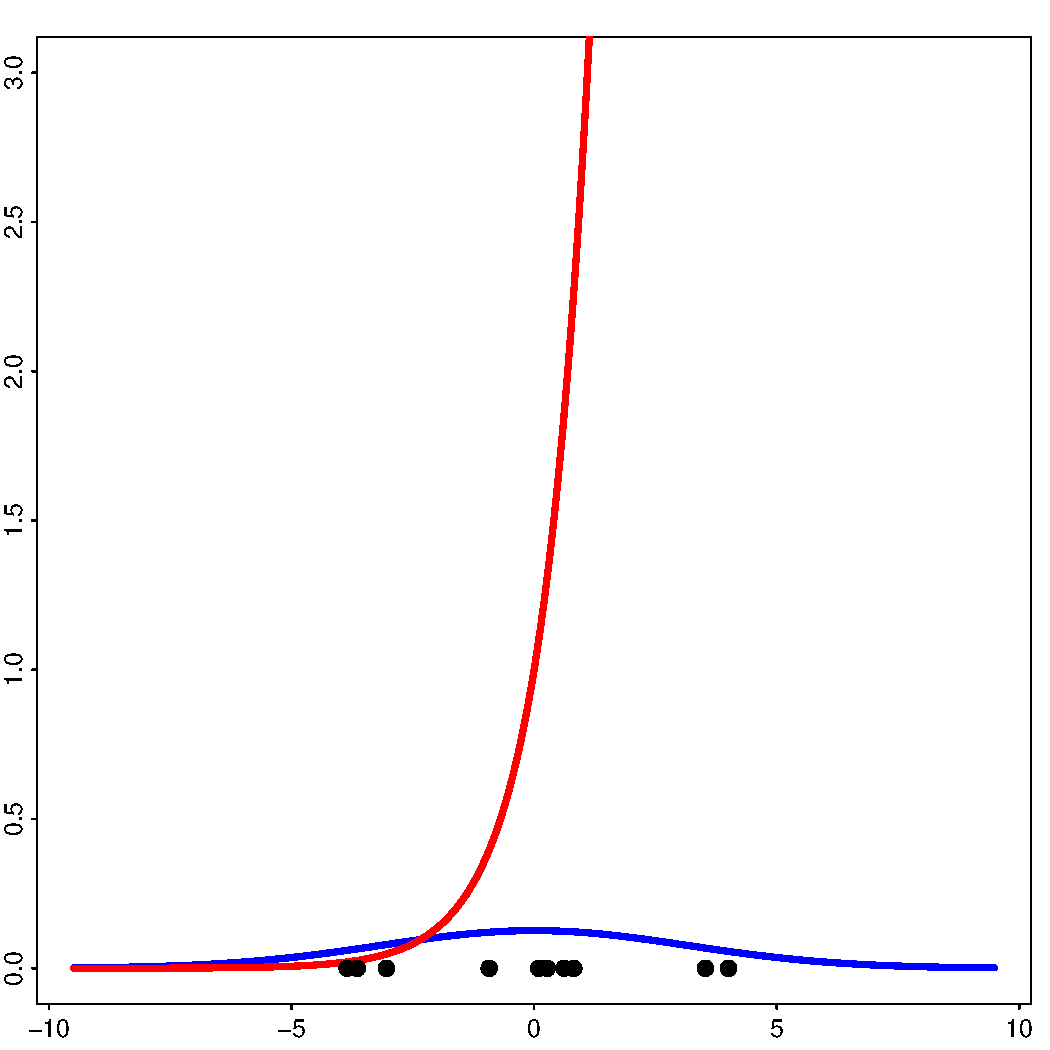
\includegraphics[width=.4\textwidth, height=.4\textheight]{../figs/EspLogNorm-MC} \\
	 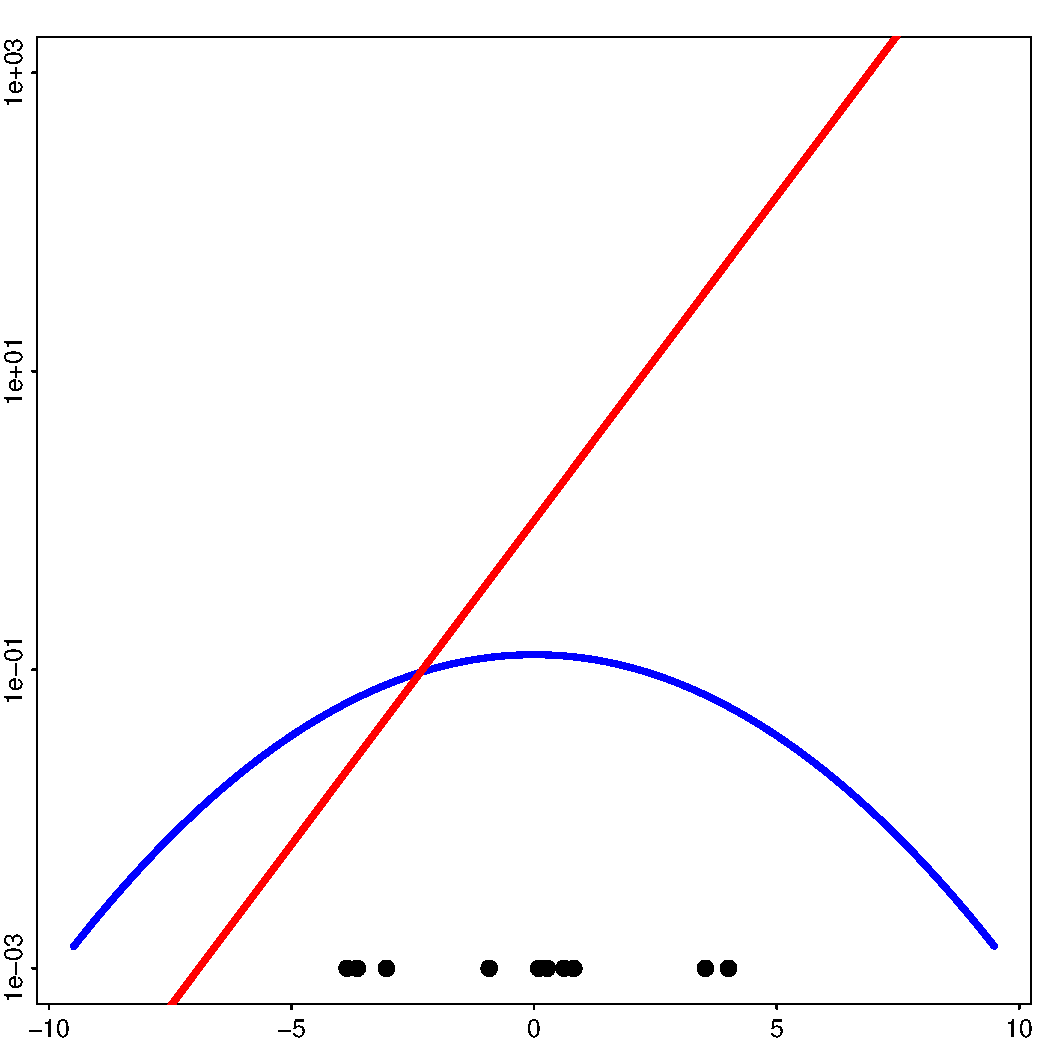
\includegraphics[width=.4\textwidth, height=.4\textheight]{../figs/EspLogNorm-MC-log} 	 
    \end{tabular}
  \end{tabular}
}






\backupend

%====================================================================
%====================================================================
\end{document}
%====================================================================
%====================================================================

  \begin{tabular}{cc}
    \begin{tabular}{p{.5\textwidth}}
    \end{tabular}
    & 
    \hspace{-.02\textwidth}
    \begin{tabular}{p{.5\textwidth}}
    \end{tabular}
  \end{tabular}

